\chapter{Агентно-ориентированные модели гибридных решателей задач ostis-систем}
\chapauthortoc{Шункевич Д.В.}
\label{chapter_situation_management}

\vspace{-7\baselineskip}

\begin{SCn}
\begin{scnrelfromlist}{автор}
	\scnitem{Шункевич Д.В.}
\end{scnrelfromlist}

\bigskip

\scntext{аннотация}{В главе сформулированы актуальные проблемы текущего состояния технологий разработки гибридных решателей задач, предложен подход к их решению на основе Технологии OSTIS. Сформулированы принципы построения решателя задач как иерархической системы навыков, основанной на многоагентном подходе, приведены онтологии агентов и выполняемых ими действий. Сформулированы принципы синхронизации деятельности агентов, а также разработана онтология базового языка программирования для реализации программ агентов и модель интерпретатора такого языка.}

\bigskip

\begin{scnrelfromlist}{подраздел}
	\scnitem{\ref{sec_ps_problems}~\nameref{sec_ps_problems}}
	\scnitem{\ref{sec_ps_actions}~\nameref{sec_ps_actions}}	
	\scnitem{\ref{sec_ps_agents}~\nameref{sec_ps_agents}}
	\scnitem{\ref{sec_ps_sync}~\nameref{sec_ps_sync}}
	\scnitem{\ref{sec_ps_scp}~\nameref{sec_ps_scp}}
	\scnitem{\ref{sec_ps_ps}~\nameref{sec_ps_ps}}
	\scnitem{\ref{sec_ps_collective}~\nameref{sec_ps_collective}}
	\scnitem{\ref{sec_ps_future}~\nameref{sec_ps_future}}
\end{scnrelfromlist}

\bigskip

\begin{scnrelfromlist}{ключевой знак}
	\scnitem{Язык SCP}
	\scnitem{Абстрактная scp-машина}
\end{scnrelfromlist}

\begin{scnrelfromlist}{ключевое понятие}
	\scnitem{действие в sc-памяти}
	\scnitem{действие в sc-памяти, инициируемое вопросом}
	\scnitem{действие редактирования базы знаний}
	\scnitem{задача, решаемая в sc-памяти}
	\scnitem{класс логически атомарных действий}
	\scnitem{sc-агент}
	\scnitem{абстрактный sc-агент}
	\scnitem{атомарный абстрактный sc-агент}
	\scnitem{неатомарный абстрактный sc-агент}
	\scnitem{абстрактный sc-агент, реализуемый на Языке SCP}
	\scnitem{абстрактный sc-агент, не реализуемый на Языке SCP}	
	\scnitem{тип блокировки}
	\scnitem{транзакция в sc-памяти}	
	\scnitem{scp-оператор}
	\scnitem{решатель задач ostis-системы}
	\scnitem{машина обработки знаний}
\end{scnrelfromlist}

\begin{scnrelfromlist}{ключевое отношение}
	\scnitem{блокировка*}
	\scnitem{планируемая блокировка*}
	\scnitem{приоритет блокировки*}
	\scnitem{удаляемые sc-элементы*}
	\scnitem{параметр scp-программы\scnrolesign}
	\scnitem{scp-операнд\scnrolesign}
\end{scnrelfromlist}

\bigskip

\begin{scnrelfromlist}{библиографическая ссылка}
	\scnitem{\scncite{Kolesnikov2001}}
	\scnitem{\scncite{Pratt2002}}
	\scnitem{\scncite{Gladkov2006}}
	\scnitem{\scncite{Emelyanov2003}}
	\scnitem{\scncite{Berkinblit1993}}
	\scnitem{\scncite{Golovko2001}}
	\scnitem{\scncite{Gorban1996}}
	\scnitem{\scncite{Vagin2008}}
	\scnitem{\scncite{Khulick2001}}
	\scnitem{\scncite{Polya1975}}
	\scnitem{\scncite{Batyrshin2001}}
	\scnitem{\scncite{Demenkov2005}}
	\scnitem{\scncite{Pospelov1989}}
	\scnitem{\scncite{Reiter1980}}
	\scnitem{\scncite{Eremeev1997}}
	\scnitem{\scncite{Kachro1988}}
	\scnitem{\scncite{Ephymov1982}}
	\scnitem{\scncite{Raghovsky2011}}
	\scnitem{\scncite{Podkholzyn2008}}
	\scnitem{\scncite{Khurbatov2016}}
	\scnitem{\scncite{Vladimirov2010}}
	\scnitem{\scncite{AIRefBookP11990}}
	\scnitem{\scncite{Jackson1998}}
	\scnitem{\scncite{W3C}}
	\scnitem{\scncite{RDF}}
	\scnitem{\scncite{OWL}}
	\scnitem{\scncite{SPARQL}}
	\scnitem{\scncite{Neo4j}}
	\scnitem{\scncite{OWLImplementations}}
	\scnitem{\scncite{Gribova2015a}}
	\scnitem{\scncite{Gribova2011}}
	\scnitem{\scncite{Phylyppov2016}}
	\scnitem{\scncite{Borisov2014}}
	\scnitem{\scncite{Dutta1993}}
	\scnitem{\scncite{Pau1990}}
	\scnitem{\scncite{Wooldridge2009}}
	\scnitem{\scncite{Weyns2007}}
	\scnitem{\scncite{ACL}}
	\scnitem{\scncite{Finin1994}}
	\scnitem{\scncite{KIF}}
	\scnitem{\scncite{Hartung2008}}
	\scnitem{\scncite{Sims2008}}
	\scnitem{\scncite{Excelente-Toledo2004}}
	\scnitem{\scncite{NagendraPrasad1999}}
	\scnitem{\scncite{Vasconcelos2009}}
	\scnitem{\scncite{Rumbell2012}}
	\scnitem{\scncite{Gorodetsky2015}}
	\scnitem{\scncite{Bordini2007}}
	\scnitem{\scncite{Castillo2014}}
	\scnitem{\scncite{EVE}}
	\scnitem{\scncite{GAMA}}
	\scnitem{\scncite{GOAL}}
	\scnitem{\scncite{Evertsz2004}}
	\scnitem{\scncite{JADE}}
	\scnitem{\scncite{Boissier2013}}
	\scnitem{\scncite{Omicini1999}}
	\scnitem{\scncite{Jagannathan1989}}
	\scnitem{\scncite{Pospelov1986}}
	\scnitem{\scncite{Dijkstra2002}}
	\scnitem{\scncite{Hoare1983}}
	\scnitem{\scncite{Chatterjee2022}}
	\scnitem{\scncite{Narinjani2004}}
	\scnitem{\scncite{Cao2010}}
	\scnitem{\scncite{Cao2014}}
	\scnitem{\scncite{Pavel2015}}
	\scnitem{\scncite{Altshuller2010}}
	\scnitem{\scncite{Shhedrovickij1995}}
	\scnitem{\scncite{Sapatyj1986}}
	\scnitem{\scncite{Moldovan1985}}
	\scnitem{\scncite{Letichevskij2003}}
	\scnitem{\scncite{Letichevskij2012}}
\end{scnrelfromlist}

\end{SCn}

\section*{Введение в Главу \ref{chapter_situation_management}}

Одним из ключевых компонентов \textit{интеллектуальной системы}, обеспечивающим возможность решать широкий круг \textit{задач}, является \textit{решатель задач}. Их особенностью по сравнению с другими современными \textit{программными системами} является необходимость решать \textit{задачи} в условиях, когда необходимые сведения не локализованы явно в \textit{базе знаний} \textit{интеллектуальной системы} и должны быть найдены в процессе решения \textit{задачи} на основании каких-либо критериев. 

Говоря другими словами, если в традиционных системах при решении задачи всегда подразумевается, что есть некоторые локализованные исходные данные ("дано") и некоторое описание желаемого результата ("что требуется"), то в \textit{интеллектуальной системе} в качестве исходных данных при решении большого числа \textit{задач} выступает вся имеющаяся на текущий момент в системе информация, то есть вся \textit{база знаний}. Кроме того, при невозможности решения задачи в текущем состоянии базы знаний интеллектуальная система должна иметь возможность понять, чего именно не хватает для продолжения процесса решения и попытаться добыть недостающие сведения во внешней среде (например, запросить у пользователя).

К настоящему времени в рамках различных направлений \textit{Искусственного интеллекта} разработано большое количество различных \textit{моделей решения задач}, каждая из которых позволяет решать задачи определенного класса. Расширение областей применения \textit{интеллектуальных систем} требует от них возможности решать так называемые \textit{комплексные задачи}, решение каждой из которых требует комбинирования нескольких моделей решения задач, при этом априори неизвестно, в каком порядке и сколько раз будет применяться так или иная модель. \textit{решатели задач}, в рамках которых комбинируются несколько \textit{моделей решения задач}, получили название \textit{гибридных решателей задач}, а интеллектуальные системы, в рамках которых комбинируются различные \textit{виды знаний} и различные \textit{модели решения задач} -- \textit{гибридных интеллектуальных систем} (см. \scncite{Kolesnikov2001}).

Повышение эффективности разработки и эксплуатации \textit{гибридных интеллектуальных систем} требует унификации моделей представления различных \textit{видов знаний} и \textit{моделей обработки знаний}, которая бы позволила легко интегрировать на ее основе компоненты, соответствующие различным моделям решения задач.

\section{Современное состояние, проблемы в области разработки гибридных решателей задач и предлагаемый подход к их решению}
\markboth{Проблемы в области разработки гибридных решателей и предлагаемый подход }{Проблемы в области разработки гибридных решателей и предлагаемый подход}
\label{sec_ps_problems}

\begin{SCn}
\begin{scnrelfromlist}{подраздел}
	\scnitem{\ref{subsec_ps_req}~\nameref{subsec_ps_req}}
	\scnitem{\ref{subsec_ps_proposed_approach}~\nameref{subsec_ps_proposed_approach}}
\end{scnrelfromlist}
\end{SCn}

\subsection{Современное состояние технологий разработки решателей задач и требования, предъявляемые к гибридным решателям задач}
\label{subsec_ps_req}

Существующее многообразие подходов к решению \textit{задач} в \textit{компьютерных системах} можно разделить на два класса:
\begin{textitemize}
	\item \textbf{решение задач с использованием хранимых программ.} В данном случае предполагается, что в системе заранее присутствует программа решения задачи заданного класса и решение сводится к поиску такой программы и интерпретации ее на заданных входных данных. К системам, ориентированным на такой подход к решению задач, относятся в том числе системы, использующие:
	\begin{textitemize}
		\item программы, написанные на языках программирования, относящихся как к императивной, так и к декларативной парадигме, в том числе логических и функциональных (см. \scncite{Pratt2002});
		\item реализации генетических алгоритмов (см. \scncite{Gladkov2006}, \scncite{Emelyanov2003});
		\item нейросетевые модели обработки знаний (см. \scncite{Berkinblit1993},\newline \scncite{Golovko2001}, \scncite{Gorban1996}).
	\end{textitemize}	
	\vspace{-2\parskip}
	Следует отметить, что даже в случае использования хранимой \textit{программы} решение \textit{задачи} далеко не всегда тривиально, поскольку, во-первых, требуется найти такую хранимую \textit{программу} на основе некоторой спецификации, во-вторых, обеспечить ее интерпретацию.
	\vspace{\parskip}
	\item \textbf{решение задач в условиях, когда программа решения не известна.} В этом случае предполагается, что в системе необязательно присутствует готовая \textit{программа} решения для \textit{класса задач}, которому принадлежит некоторая сформулированная задача, подлежащая решению. В связи с этим необходимо применять дополнительные методы поиска путей решения задачи, не рассчитанные на какой-либо узкий \textit{класс задач} (например, разбиение задачи на подзадачи, методы поиска решений в глубину и ширину, метод случайного поиска решения и метод проб и ошибок, метод деления пополам и другие), а также различные модели \textit{логического вывода}: классические дедуктивные (см. \scncite{Vagin2008}), индуктивные (см. \scncite{Khulick2001}, \scncite{Polya1975}), абдуктивные (см. \scncite{Vagin2008}); модели, основанные на \textit{нечетких логиках} (см. \scncite{Batyrshin2001}, \scncite{Demenkov2005}, \scncite{Pospelov1989}), \textit{логике умолчаний} (см. \scncite{Reiter1980}), \textit{темпоральной логике} (см. \scncite{Eremeev1997}), и многие другие.
\end{textitemize}

Подробный обзор \textit{решателей задач}, разработанных в период до 1982 года, таких как \textit{GPS}, \textit{STRIPS}, \textit{QA3}, \textit{ПРИЗ} (см. \scncite{Kachro1988}), \textit{ППР} приведен в книге \scncite{Ephymov1982}. Среди современных работ, исследующих вопросы применения \textit{моделей решения задач}, не ориентированных на конкретную предметную область, можно выделить \scncite{Raghovsky2011}. Среди наиболее заметных представителей класса \textit{интеллектуальных решателей задач}, разработанных в более поздний период, можно отметить \textit{Компьютерный решатель математических задач} (см. \scncite{Podkholzyn2008}), \textit{Решатель задач по планиметрии НИЦ ЭВТ} (см. \scncite{Khurbatov2016}), \textit{Программный комплекс ``УДАВ''} (см. \scncite{Vladimirov2010}). 

Отдельного внимания заслуживают популярные в настоящее время \textit{системы компьютерной алгебры}, такие как \textit{Wolfram Mathematica}, \textit{Maple}, \textit{MathCAD} и другие. Указанные программные комплексы обладают мощной функциональностью как для проведения различного рода вычислений и экспериментов, так и для построения на их основе систем различного назначения, например обучающих. Более подробно возможности применения систем данного семейства для решения \textit{задач} в рамках \textit{Экосистемы OSTIS} рассмотрены в \textit{\ref{sec_integration_algebra}~\nameref{sec_integration_algebra}}.

Однако при всем многообразии решаемых рассмотренными системами \textit{задач} множество \textit{классов задач} ограничивается имеющимся в системе набором жестко заданных приемов и алгоритмов решения \textit{задач}, явно используемых при решении той или иной \textit{задачи}. В то же время построение сложных систем, например, систем комплексной автоматизации, невозможно без обеспечения согласованного использования различных \textit{видов знаний} и \textit{моделей решения задач} в рамках одной системы при решении одной и той же \textit{комплексной задачи}. Кроме того, становится актуальной \textit{задача} поддержки такой системы в состоянии, соответствующем текущему уровню развития технологий, дополнения ее более совершенными \textit{моделями} и \textit{методами решения задач}. При этом очевидно, что подобная реконфигурация системы должна осуществляться \myuline{непосредственно в процессе эксплуатации системы}, а не требовать каждый раз, например, полной остановки всего производства или отдельных его частей.

Сказанное выше позволяет сформулировать требования \textit{гибридному решателю задач}:
\begin{textitemize}
	\item в каждый момент времени \textit{решатель задач} должен обеспечивать решение задач из оговоренного класса за оговоренное время, при этом результат решения задачи должен удовлетворять некоторым известным требованиям. Другими словами, как и в случае современных \textit{компьютерных систем}, корректность результатов решения задач на этапе разработки системы должна верифицироваться специальными методами, в том числе для этого могут быть использованы такие современные подходы, как \textit{unit-тестирование}, \textit{тестирование методом «черного ящика}» и другие. Более детально рассмотрим положения, уточняющие сформулированное требование:
	\begin{textitemize}
		\item для явно сформулированных \textit{задач} система всегда должна давать какой-либо ответ за оговоренное время, при этом ответ может быть отрицательным (система не смогла решить поставленную задачу), возможно, с объяснением причин, по которым решение в текущий момент оказалось невозможным. Одним из факторов безуспешности решения является выход за рамки установленного промежутка времени;
		\item если явно сформулированная \textit{задача} решена, то все \textit{информационные процессы}, направленные на ее решение, должны быть уничтожены. Особенно актуальным данное требование становится в ситуации, когда для решения одной и той же задачи параллельно используются сразу несколько подходов и заранее неизвестно, какой из них приведет к результату раньше других;
		\item после решения задачи вся временная информация, сгенерированная в процессе решения этой \textit{задачи} и имеющая ценность только в контексте решения указанной \textit{задачи}, должна быть удалена из памяти;
	\end{textitemize}
	
	\item \textit{\textbf{гибридный решатель}} должен обеспечивать возможность \textbf{согласованного использования различных моделей решения задач} при решении одной и той же \textit{комплексной задачи} в случае необходимости;
	
	\item \textit{решатель задач} должен быть легко \textbf{модифицируемым}, то есть трудоемкость внесения изменений в уже разработанный \textit{решатель задач} должна быть минимальна. Путями повышения модифицируемости \textit{решателя задач} являются обеспечение локальности вносимых изменений, в том числе -- за счет стратификации \textit{решателя задач} на независимые уровни и обеспечение максимальной независимости компонентов \textit{решателя задач} друг от друга, а также наличие готовых компонентов, которые могут быть встроены в \textit{решатель задач} при необходимости. При этом внесение изменений должно осуществляться \myuline{непосредственно в процессе эксплуатации системы};
	
	\item для того чтобы \textit{интеллектуальная система} имела возможность анализировать и оптимизировать имеющийся \textit{решатель задач}, интегрировать в его состав новые компоненты (в том числе самостоятельно), оценивать важность тех или иных компонентов и применимость их для решения той или иной задачи, спецификация \textit{решателя задач} должна быть описана языком, понятным системе, например, при помощи тех же средств, что и обрабатываемые \textit{знания}. Другими словами, \textit{интеллектуальная система} и, соответственно, \textit{решатель задач} должны обладать \textit{рефлексивностью}.
\end{textitemize}

Несмотря на то что в настоящее время существует большое число \textit{моделей решения задач}, многие из которых реализованы и успешно используются на практике в различных системах, остается актуальной проблема низкой согласованности принципов, лежащих в основе реализации таких моделей, и отсутствия единой унифицированной основы для реализации и интеграции различных \textit{моделей решения задач}, что приводит к тому, что:

\begin{textitemize}
	\item затруднена возможность одновременного использования различных \textit{моделей решения задач} в рамках одной системы при решении одной и той же комплексной задачи; практически невозможно комбинировать различные модели с целью решения \textit{задачи}, для которой априори отсутствует \textit{алгоритм} ее решения;
	\item практически невозможно использовать технические решения, реализованные в одной системе, в других системах, то есть возможности использования компонентного подхода при построении \textit{решателей задач} сильно ограничены. Как следствие, велико количество дублирований аналогичных решений в разных системах;
	\item фактически отсутствуют комплексные методики и средства построения \textit{решателей задач}, которые бы обеспечивали возможность проектирования, реализации и отладки \textit{решателей задач} различного вида.
\end{textitemize}

Следствиями указанных проблем являются:

\begin{textitemize}
\item высокая трудоемкость разработки каждого \textit{решателя задач}, увеличение сроков их разработки, а значит, и увеличение затрат на разработку и поддержку соответствующих \textit{интеллектуальных систем};
\item высокая трудоемкость внесения изменений в уже разработанные \textit{решатели задач}, то есть отсутствует или сильно затруднена возможность дополнения уже разработанного \textit{решателя задач} новыми компонентами и внесения изменений в уже существующие компоненты в процессе эксплуатации системы. Таким образом, высока трудоемкость поддержки разработанных \textit{решателей задач};
\item высокий уровень профессиональных требований к разработчикам \textit{решателей задач}, что обусловлено, в частности:
	\begin{textitemize}
	\item высокой сложностью существующих формализмов в области решения \textit{задач}, рассчитанных на их интерпретацию \textit{компьютерной системой}, а не человеком;
	\item отсутствием возможности рассматривать разрабатываемые \textit{решатели задач} на разных уровнях детализации, выделения на каждом уровне достаточно независимых компонентов, что затрудняет процесс проектирования, тестирования и отладки таких \textit{решателей задач}, а также снижает эффективность попыток объединения разработчиков \textit{решателей задач} в коллективы по причине увеличения накладных расходов на согласование их деятельности;
	\item низким уровнем информационной поддержки разработчиков и автоматизации их \textit{деятельности}.
\end{textitemize}
\end{textitemize}

Для решения перечисленных проблем необходимо разработать комплекс моделей, методики и средств разработки \textit{гибридных решателей задач}, удовлетворяющих перечисленным ранее требованиям.

Исторически сложились два основных подхода к построению \textit{решателей задач} \textit{интеллектуальных компьютерных систем}.

Первый подход предполагает наличие в системе фиксированного \textit{решателя задач} (например, машины логического вывода), к которому впоследствии добавляется \textit{база знаний}, наполнение которой определяется \textit{предметной областью}, в которой должна работать система. Такие системы получили название "пустых"{} \textit{экспертных систем} (см. \scncite{AIRefBookP11990}) или "оболочек"{} (expert system shells, см. \scncite{Jackson1998}). Данный подход, как правило, использовался для разработки относительно несложных систем и в настоящее время не имеет широкого применения.

Второй подход, широко используемый в настоящее время, предполагает наличие программных средств доступа к информации, хранящейся в некоторой базе, совместимых с различными популярными \textit{языками программирования}. Данный подход широко используется, например, в системах, построенных на основе стандартов \textit{W3C} (см. \scncite{W3C}), таких как \textit{RDF} (см. \scncite{RDF}), \textit{OWL} (см. \scncite{OWL}), \textit{SPARQL} (см. \scncite{SPARQL}), а также \textit{графовых с.у.б.д.}, таких как \textit{Neo4j} (см. \scncite{Neo4j}). Структура \textit{решателя задач}, построенного на базе таких средств, определяется разработчиком в каждом конкретном случае и не фиксируется какими-либо стандартами. Такой подход обладает большей гибкостью, но отсутствие унификации в структуре и процессе разработки \textit{решателей задач} приводит к отсутствию совместимости компонентов \textit{решателей задач}, созданных разными разработчиками, большому количеству дублирований одних и тех же решений, повышению накладных расходов в процессе разработки и поддержки \textit{решателя задач}. Также существует большое количество реализаций так называемых \textit{ризонеров} (semantic reasoners), осуществляющих \textit{логический вывод} на \textit{онтологиях}, представленных в формате \textit{OWL 2}, а также средств разработки и редактирования таких \textit{онтологий}. Полный список таких средств, признанных консорциумом \textit{W3C}, можно найти на сайте \scncite{OWLImplementations}. Как видно из приведенной на нем таблицы, подавляющее большинство средств способно осуществлять только прямой \textit{логический вывод} на основе \textit{отношений}, описанных в \textit{онтологии}.

Среди комплексных подходов к построению \textit{решателей задач}, разрабатываемых русскоязычными авторами, можно выделить проект \textit{IACPaaS} (см. \scncite{Gribova2015a},  \scncite{Gribova2011}), активно развивающийся в настоящее время. Целью данного проекта является разработка облачной платформы для построения на ее основе \textit{интеллектуальных сервисов} различного назначения. В данном проекте активно используются \textit{библиотеки многократно используемых компонентов интеллектуальных систем}. Конкретно для построения \textit{решателей задач}, а также \textit{пользовательских интерфейсов} таких систем используется \textit{многоагентный подход}. Несмотря на близость некоторых технологических решений, реализуемых в проекте \textit{IACPaaS} и в рамках \textit{Технологии OSTIS}, основной целью указанного проекта является предоставление пользователю большого числа разнородных сервисов, выбор которых осуществляется самим пользователем, в то время как одним из ключевых принципов \textit{Технологии OSTIS} является разработка общей формальной основы для интеграции различных \textit{моделей решения задач} с целью их комбинирования при решении одной и той же \textit{комплексной задачи}.

Задачи интеграции различных подходов, в том числе связанных с решением задач, исследуются также в работе \scncite{Phylyppov2016} и других работах тех же авторов.

Компонентному проектированию \textit{интеллектуальных систем, основанных на знаниях}, посвящена работа \scncite{Borisov2014}, в которой обосновывается необходимость накопления и повторного использования различных компонентов \textit{интеллектуальных систем}, предлагаются возможные решения данной проблемы с использованием \textit{онтологий}.

Состояние работ англоязычных авторов, посвященных вопросам решения задач в \textit{системах, основанных на знаниях}, и актуальных на момент начала 1990-х годах, отражено в обзорных публикациях \scncite{Dutta1993}, \scncite{Pau1990}. Более поздние англоязычные работы в данной области в основном ориентированы на решение конкретных частных \textit{задач} в системах, построенных на основе стандартов \textit{W3C}, о которых более подробно было сказано выше.

Таким образом, можно сказать, что существует ряд конкретных разработок в направлении построения \textit{комплексных технологий разработки интеллектуальных систем} различных классов, в том числе с использованием \textit{библиотек многократно используемых компонентов}, однако проблема разработки комплексной технологии построения \textit{гибридных решателей задач} в рамках рассмотренных подходов не решена. Во многом это обусловлено отсутствием унифицированной формальной основы для представления любых \textit{видов знаний}, в том числе различного рода программ, отсутствием строгих принципов, регламентирующих процесс построения \textit{решателей задач}, а также средств поддержки разработчиков таких \textit{решателей задач} и их компонентов.

\subsection{Предлагаемый подход к разработке гибридных решателей задач ostis-систем и обработке информации в ostis-системах}
\label{subsec_ps_proposed_approach}

Рассмотрим принципы, лежащие в основе предлагаемого подхода к разработке \textit{гибридных решателей задач}:

\begin{textitemize}
\item в качестве основы для построения модели гибридного \textit{решателя задач} предлагается использовать \textit{многоагентный подход}. Данный подход позволяет обеспечить основу для построения параллельных асинхронных систем, имеющих распределенную архитектуру, повысить модифицируемость и производительность разработанных \textit{решателей задач};
\item процесс решения любой \textit{задачи} предлагается декомпозировать на \textit{логически атомарные действия}, что также позволит обеспечить совместимость и модифицируемость \textit{решателей задач};
\item \textit{решатель задач} (как объединенный, так и \textit{решатель задач} частного вида) предлагается рассматривать как иерархическую систему, состоящую из нескольких взаимосвязанных уровней. Такой подход позволяет обеспечить возможность проектирования, отладки и верификации компонентов на разных уровнях независимо от других уровней, что существенно упрощает задачу построения \textit{решателя задач} за счет снижения накладных расходов;
\item предлагается записывать \myuline{всю} информацию о решателе и решаемых им задачах при помощи \textit{SC-кода} в той же \textit{базе знаний}, что и собственно предметные \textit{знания} системы. В общем случае такая информация включает: 

	\begin{textitemize}
	\item \textit{спецификацию агентов}, входящих в состав \textit{решателя задач}; 
	\item \textit{спецификацию методов}, интерпретируемых \textit{агентами} \textit{решателя задач}; 
	\item спецификацию всех \textit{информационных процессов}, выполняемых агентами в \textit{семантической памяти}, в том числе -- конструкции, обеспечивающие синхронизацию выполнения параллельных процессов;
	\item спецификацию всех \textit{задач}, на решение которых направлены указанные \textit{информационные процессы}. 
	\end{textitemize}

Описание всей указанной информации в единой семантической  памяти позволит, во-первых, обеспечить независимость разрабатываемых \textit{решателей задач} от \textit{ostis-платформы} (см. \textit{Главу \ref{chapter_interpreter}~\nameref{chapter_interpreter}}), во-вторых, обеспечить возможность системы анализировать происходящие в ней процессы, оптимизировать и синхронизировать их выполнение, то есть обеспечить \textit{рефлексивность} проектируемых \textit{интеллектуальных систем}.
\end{textitemize}

Ориентация на \textit{многоагентный подход} как основу для построения \textit{гибридных решателей задач} обусловлена следующими основными преимуществами такого подхода (см. \scncite{Wooldridge2009}):
\begin{textitemize}
\item автономность (независимость) \textit{агентов} в рамках такой системы, что позволяет локализовать изменения, вносимые в \textit{решатель задач} при его эволюции, и снизить соответствующие трудозатраты, а также обеспечить устойчивость такой системы к отказам некоторых агентов;
\item децентрализация обработки, то есть отсутствие единого контролирующего центра, что также позволяет локализовать вносимые в \textit{решатель задач} изменения;
\item возможность параллельной работы разных \textit{информационных процессов}, соответствующих как одному \textit{агенту}, так и разным агентам, как следствие, -- возможность распределенного решения задач. Однако возможность параллельного выполнения \textit{информационных процессов} подразумевает наличие средств синхронизации такого выполнения, разработка которых является отдельной задачей и подробно рассматривается ниже;
\item активность \textit{агентов} и \textit{многоагентной системы} в целом, дающая возможность при общении с такой системой не указывать явно способ решения поставленной \textit{задачи}, а формулировать задачу в \textbf{декларативном ключе}.
\end{textitemize}

Построение модели \textit{многоагентной системы} требует уточнения модели каждого компонента, входящего в ее состав, а именно:
\begin{textitemize}
\item \textbf{модель собственно агента}, входящего в состав такой системы, включая классификацию таких \textit{агентов} и набор понятий, характеризующих каждый агент в рамках системы. В настоящее время наиболее популярной является модель \textit{BDI} (belief-desire-intention), в рамках которой предполагается описывать на соответствующих языках "убеждения"{}, "желания"{} и "намерения"{} каждого агента системы;
\item \textbf{модель среды}, в рамках которой находятся агенты, на события в которой они реагируют и в рамках которой могут осуществлять некоторые преобразования. Обзор разновидностей сред для многоагентных систем приводится в работе \scncite{Weyns2007};
\item \textbf{модель коммуникации агентов}, в рамках которой уточняется язык взаимодействия \textit{агентов} (структура и классификация сообщений) и способ передачи сообщений между \textit{агентами}.
\end{textitemize}

В свою очередь, для разработки модели коммуникации \textit{агентов} необходимо отдельно уточнить каждый из ее компонентов:

\begin{textitemize}
\item \textbf{Принципы обмена сообщениями между агентами}, то есть то, каким образом эти сообщения передаются от \textit{агента} к \textit{агенту};
\item \textbf{Классификацию, семантику и прагматику таких сообщений}, то есть \textit{смысл} передаваемой информации и цель такого взаимодействия. В настоящее время стандартами, описывающими структуру передаваемых агентами сообщений, являются \textit{Agent Communication Language} (\textit{ACL}) (см. \scncite{ACL}), разработанный сообществом \textit{FIPA}, язык \textit{KQML} (см. \scncite{Finin1994}). Указанные стандарты уточняют базовые компоненты каждого сообщения (кодировка, язык сообщения, используемую онтологию понятий, получателя, отправителя и так далее), не ограничивая при этом \textit{смысл} сообщения в целом. Также для коммуникации между агентами используется язык \textit{KIF}, предназначенный для обмена \textit{знаниями} между любыми программными компонентами (см. \scncite{KIF}); 
\item \textbf{Принципы координации деятельности агентов}
В литературе рассматривается большое число вариантов координации деятельности \textit{агентов}. В работе \scncite{Hartung2008} предлагается выделить агенты более высокого уровня (\textit{метаагенты}), \textit{задачей} которых является сбор информации от \textit{агентов} нижнего уровня и их координация, схожие идеи высказываются в работе \scncite{Sims2008}. В работах \scncite{Excelente-Toledo2004}, \scncite{NagendraPrasad1999} предлагаются варианты автоматического выбора оптимального механизма координации \textit{агентов} для достижения общей цели. Предлагаются также социально-психологические модели координации деятельности \textit{агентов}, например, на основе некоторых общих "законов"{} (см. \scncite{Vasconcelos2009}) или эмоций (см. \scncite{Rumbell2012}). В работе \scncite{Gorodetsky2015} предложен вариант онтологии коллективного поведения автономных \textit{агентов}.
\end{textitemize}

К основным недостаткам большинства популярных современных средств построения \textit{многагентных систем} (см. \scncite{Bordini2007}, \scncite{Castillo2014}, \scncite{EVE}, \scncite{GAMA},	\scncite{GOAL}, \scncite{Evertsz2004}, \scncite{JADE}, \scncite{Boissier2013}) можно отнести следующие:
\begin{textitemize}
\item жесткая ориентация большинства средств на модель \textit{BDI} приводит к существенным накладным расходам, связанным с необходимостью выражения конкретной практической \textit{задачи} в системе понятий \textit{BDI}. В то же время ориентация на модель \textit{BDI} неявно провоцирует искусственное разделение языков, описывающих собственно компоненты \textit{BDI} и знания \textit{агента} о внешней среде, что приводит к отсутствию \textit{унификации представления} и, соответственно, дополнительным накладным расходам;
\item большинство современных средств построения \textit{многоагентных систем} ориентированы на представление \textit{знаний} \textit{агента} при помощи узкоспециализированных языков, зачастую не предназначенных для представления \textit{знаний} в широком смысле. Речь при этом идет как о знаниях агента о себе самом, так и \textit{знаниях} о внешней среде. В некоторых подходах вначале строится онтология, для создания которой, однако, часто используются средства с низкой выразительной способностью, не предназначенные для построения \textit{онтологий} (см. \scncite{Evertsz2004}, \scncite{JADE}). В конечном итоге такой подход приводит к сильной ограниченности возможностей построенных \textit{многоагентных систем} и их несовместимости;
\item абсолютное большинство современных средств предполагает, что взаимодействие \textit{агентов} осуществляется путем обмена сообщениями непосредственно от \textit{агента} к \textit{агенту} или посредством специальных коммуникационных центров (см. \scncite{Omicini1999}), например, в случае взаимодействия \textit{агентов} в глобальной сети. Такой подход обладает существенным недостатком, связанным с тем, что в этом случае каждый \textit{агент} системы должен иметь достаточно полную информацию о других агентах в системе, что приводит к дополнительным затратам ресурсов, кроме того, добавление или удаление одного или нескольких \textit{агентов} приводит к необходимости оповещения об этом других \textit{агентов}. Данная проблема решается путем организации общения агентов по принципу "доски объявлений"{} (см. \scncite{Jagannathan1989}), предполагающему, что сообщения помещаются в некоторую общую для всех агентов область, при этом каждый \textit{агент} в общем случае может не знать, какому из агентов адресовано сообщение и от какого из \textit{агентов} получено то или иное сообщение. Кроме того, в построенной таким образом системе легче обеспечивается параллельное решение несвязанных друг с другом \textit{задач}, поскольку сообщения, относящиеся к одной \textit{задаче}, будут игнорироваться агентами, решающими другую задачу. Однако данный подход не исключает проблему, связанную с необходимостью разработки специализированного языка взаимодействия \textit{агентов}, который в общем случае не связан с языком, на котором описываются \textit{знания} \textit{агента} о решаемых \textit{задачах} и окружающей среде;
\item многие средства построения \textit{многоагентных систем} построены таким образом, что логический уровень взаимодействия \textit{агентов} жестко привязан к физическому уровню реализации \textit{многоагентной системы}. Например, при передаче сообщений от агента к агенту разработчику \textit{многоагентной системы} необходимо помимо семантически значимой информации указывать ip-адрес компьютера, на котором расположен \textit{агент-получатель}, кодировку, с помощью которой закодирован текст сообщения, и другую техническую информацию, обусловленную исключительно особенностями текущей реализации средств;
\item в большинстве подходов среда, с которой взаимодействуют \textit{агенты}, уточняется отдельно разработчиком для каждой \textit{многоагентной системы}, что с одной стороны, расширяет возможности применения соответствующих средств, но, с другой стороны, приводит к существенным накладным расходам и несовместимости таких многоагентных систем. Кроме того, в ряде случаев разработчик также обязан учитывать особенности технической реализации средств разработки в плане их стыковки с предполагаемой средой, в роли которой может выступать, например, локальная или глобальная сеть.
\end{textitemize}

Перечисленные недостатки предполагается устранять за счет использования следующих принципов:
\begin{textitemize}
\item коммуникацию агентов предлагается осуществлять по принципу \textit{"доски объявлений"{}}, однако в отличие от классического подхода в роли сообщений выступают спецификации в общей семантической памяти выполняемых \textit{агентами} \textit{действий}, направленных на решение каких-либо задач, а в роли среды коммуникации выступает сама эта \textit{семантическая память}. Такой подход позволяет: 
	\begin{textitemize}
	\item исключить необходимость разработки специализированного языка для обмена сообщениями;
	\item обеспечить "обезличенность"{} общения, то есть каждый из \textit{агентов} в общем случае не знает, какие еще агенты есть в системе, кем сформулирован и кому адресован тот или иной запрос. Таким образом, добавление или удаление агентов в систему не приводит к изменениям в других \textit{агентах}, что обеспечивает модифицируемость всей системы;
	\item агентам, в том числе конечному пользователю, формулировать задачи в \textit{декларативном ключе}, то есть не указывать для каждой задачи способ ее решения. Таким образом, агенту заранее не нужно знать, каким образом система решит ту или иную задачу, достаточно лишь специфицировать конечный результат;
	\item сделать средства коммуникации \textit{агентов} и синхронизации их деятельности более понятными разработчику и пользователю системы, не требующими изучения специальных низкоуровневых типов данных и форматов сообщений. Таким образом повышается доступность предлагаемых решений широкому кругу разработчиков.
	\end{textitemize}
\vspace{-2\parskip}
Следует отметить, что такой подход позволяет при необходимости организовать обмен сообщениями между \textit{агентами} напрямую и, таким образом, может являться основой для моделирования многоагентных систем, предполагающих другие способы взаимодействия между \textit{агентами}.
\vspace{\parskip}
\item в роли внешней среды для агентов выступает та же \textit{семантическая память}, в которой формулируются задачи и посредством которой осуществляется взаимодействие \textit{агентов}. Такой подход обеспечивает унификацию среды для различных систем \textit{агентов}, что, в свою очередь, обеспечивает их совместимость;
\item спецификация каждого агента описывается средствами \textit{SC-кода} в \textit{базе знаний}, что позволяет:
	\begin{textitemize}
	\item минимизировать число специализированных средств, необходимых для спецификации агентов, как языковых, так и инструментальных;
	\item с одной стороны -- минимизировать необходимую в общем случае спецификацию агента, которая включает условие его инициирования и \textit{программу}, описывающую алгоритм работы \textit{агента}, с другой стороны -- обеспечить возможность произвольного расширения спецификации для каждого конкретного случая, в том числе возможность реализации модели \textit{BDI} и других;
	\end{textitemize}
\item синхронизацию деятельности \textit{агентов} предполагается осуществлять на уровне выполняемых ими процессов, направленных на решений тех или иных задач в \textit{семантической памяти}. Таким образом, каждый агент трактуется как некий абстрактный процессор, способный решать задачи определенного класса. При таком подходе необходимо решить задачу обеспечения взаимодействия параллельных асинхронных процессов в общей \textit{семантической памяти}, для решения которой можно заимствовать и адаптировать решения, применяемые в традиционной \textit{линейной памяти}. При этом вводится дополнительный класс агентов -- \textit{метаагенты}, задачей которых является решение возникающих проблемных ситуаций, таких как \textit{взаимоблокировки};
\item каждый \textit{информационный процесс} в любой момент времени имеет ассоциативный доступ к необходимым фрагментам \textit{базы знаний}, хранящейся в семантической памяти, за исключением фрагментов, заблокированных другими процессами в соответствии  с рассмотренным ниже механизмом синхронизации. Таким образом, с одной стороны, исключается необходимость хранения каждым агентом информации о внешней среде, с другой стороны, каждый \textit{агент}, как и в классических \textit{многоагентных системах}, обладает только частью всей информации, необходимой для решения задачи. 
	
Важно отметить, что в общем случае невозможно априори предсказать, какие именно знания, модели и способы решения задач понадобятся системе для решения конкретной задачи. В связи с этим необходимо обеспечить, с одной стороны, возможность доступа ко всем необходимым фрагментам \textit{базы знаний} (в пределе -- ко всей \textit{базе знаний}), с другой стороны -- иметь возможность локализовать область поиска пути решения \textit{задачи}, например, рамками одной \textit{предметной области}.
	
Каждый из \textit{агентов} обладает набором ключевых элементов (как правило, понятий), которые он использует в качестве отправных точек при ассоциативном поиске в рамках \textit{базы знаний}. Набор таких элементов для каждого \textit{агента} уточняется на этапах проектирования \textit{решателя задач}. Уменьшение числа ключевых элементов \textit{агента} делает его более универсальным, однако снижает эффективность его работы за счет необходимости выполнения дополнительных операций.
\end{textitemize}

Кроме \textit{многоагентного подхода}, в основу принципов решения задачи в рамках \textit{Технологии OSTIS} предлагается положить ряд идей, связанных с концепцией \textit{ситуационного управления}, рассмотренной в работе \textit{Д.А. Поспелова} \scncite{Pospelov1986}. До настоящего времени попытки реализации указанной концепции, несмотря на ее актуальность и востребованность, сводились к частным решениям для конкретных \textit{классов задач} и, к сожалению, не получили широкого распространения. В значительной степени это обусловлено отсутствием универсальной унифицированной основы, которая бы позволила на ее базе создавать языки ситуационного управления в применении к конкретным предметным областям и, что еще более важно, повторно использовать фрагменты описаний на таких языках.

Данную проблему можно решить используя предлагаемый в рамках \textit{Технологии OSTIS} \textit{SC-код} и семейство \textit{онтологий верхнего уровня}, разработанных на его основе. В частности, реализации идей ситуационного управления способствуют такие принципы, как:
\begin{textitemize}
	\item \textit{SC-код} как базовый язык для описания любой информации в \textit{базе знаний} и, соответственно, для построения языков ситуационного управления на его основе;
	\item \textit{Базовая денотационная семантика \textit{SC-кода}}, которая позволяет обеспечить возможность формального уточнения всех используемых понятий в виде формального набора \textit{онтологий}, что позволяет обеспечить совместимость разрабатываемых систем и возможность повторного использования их компонентов;
	\item \textit{агентно-ориентированный подход} к обработке информации, предполагающий реакцию \textit{агентов} на возникновение в \textit{базе знаний} определенных \textit{ситуаций} и \textit{событий}.
\end{textitemize}

Учитывая рассмотренные выше принципы реализации \textit{многоагентного подхода} и \textit{ситуационного управления} в рамках \textit{Технологии OSTIS}, сформулируем более детально основные принципы, лежащие в основе подхода к обработке информации, предлагаемого в \textit{Технологии OSTIS}:

\begin{textitemize}
	\item В основе \textit{решателя задач} каждой \textit{ostis-системы} лежит многоагентная система, агенты которой взаимодействуют между собой \uline{только}(!) через общую для них \textit{sc-память} посредством спецификации в этой памяти выполняемых ими \textit{действий в sc-памяти}. При этом пользователи \textit{ostis-системы} также считаются \textit{агентами} этой системы. Кроме того, \textbf{\textit{sc-агенты}} делятся на внутренние, рецепторные и эффекторные. Взаимодействие между \textit{агентами} через общую \textbf{\textit{sc-память}} сводится к следующим видам действий:
	\begin{textitemize}
		\item К использованию общедоступной для соответствующей группы \textit{sc-агентов} части хранимой \textit{базы знаний};
		\item К формированию (генерации) новых фрагментов \textit{базы знаний} и/или к корректировке (редактированию) каких-либо фрагментов доступной части \textit{базы знаний};
		\item К интеграции (погружению) новых (обновленных) фрагментов в состав доступной части \textit{базы знаний};
	\end{textitemize}
	\vspace{-2\parskip}
	Подчеркнем, что \textit{sc-агенты} не общаются между собой напрямую путем отправки сообщений, как это делается в большинстве современных подходов к построению \textit{многоагентных систем}. Кроме того, \textit{sc-агенты} имеют доступ к общей для них базе знаний за счет чего гарантируется семантическая совместимость (взаимопонимание) между агентами, включая и пользователей \textit{ostis-систем}.
	\vspace{\parskip}
	\item Пользователь \textit{ostis-системы} не может сам непосредственно выполнить какое-либо \textit{действие} в \mbox{sc-памяти}, но он может средствами \textit{пользовательского интерфейса} инициировать построение (генерацию, формирование в \textit{sc-памяти}) \textit{sc-текста}, являющегося спецификацией \textit{действия в \mbox{sc-памяти}}, выполняемого либо одним \textit{атомарным sc-агентом} за один акт, либо одним \textit{атомарным sc-агентом} за несколько актов, либо коллективом \textit{sc-агентов} (\textit{неатомарным sc-агентом}). В спецификации каждого такого \textit{действия в sc-памяти}, инициированного пользователем, этот пользователь указывается как заказчик этого действия. Таким образом, пользователь \textit{ostis-системы} дает поручения (задания, команды) \textit{sc-агентам} этой системы на выполнение различных специфицируемых им действий в \textit{sc-памяти}.
	
	\item Каждый \textit{sc-агент}, выполняя некоторое \textit{действие в sc-памяти}, должен "помнить"{}, что \textit{sc-память}, над которой он работает, является общим ресурсом не только для него, но и для всех остальных \textit{\mbox{sc-агентов}}, работающих над этой же \textit{sc-памятью}. Поэтому \textit{sc-агент} должен соблюдать определенную этику поведения в коллективе таких \textit{sc-агентов}, которая должна минимизировать помехи, которые он создает другим \textit{sc-агентам}.
	
	\item Деятельность каждого агента \textit{ostis-системы} дискретна и представляет собой множество элементарных действий (актов). При этом при выполнении каждого акта агент может устанавливать блокировки нескольких типов на фрагменты базы знаний. Указанные блокировки позволяют запретить другим агентам изменять указанный фрагмент базы знаний или вообще сделать его "невидимым"{} для других агентов. Блокировки устанавливаются самим агентом при выполнении соответствующего акта и снимаются им же на последнем этапе выполнения этого акта или раньше, если это возможно.
	\item Если некий \textit{sc-агент} выполняет некоторое \textit{действие в sc-памяти}, то он на время выполнения этого действия может:
	\begin{textitemize}
		\item Запретить другим \textit{sc-агентам} изменять состояние некоторых sc-элементов, хранимых в \textit{sc-памяти} -- удалять их, изменять тип;
		\item Запретить другим \textit{sc-агентам} добавлять или удалять элементы некоторых множеств, обозначаемых соответствующими \textit{sc-узлами};
		\item Запретить другим \textit{sc-агентам} доступ на просмотр некоторых \textit{sc-элементов}, то есть эти \textit{\mbox{sc-элементы}} становятся полностью "невидимыми"{} (полностью заблокированными) для других \textit{sc-агентов} но только на время выполнения соответствующего \textit{действия}.
	\end{textitemize}
	\vspace{-2\parskip}
	Указанные блокировки должны быть полностью сняты до завершения выполнения соответствующего \textit{действия}. Подчеркнем, что число \textit{sc-элементов}, блокируемых на время выполнения некоторого действия, в основном входят атомарные и неатомарные связки, и не должны входить \textit{sc-узлы}, обозначающие бесконечные классы каких-либо сущностей, и, тем более, \textit{sc-узлы}, обозначающие различные \textit{понятия} (ключевые классы различных предметных областей).
	\vspace{\parskip}
	Этичное (неэгоистичное) поведение \textit{sc-агента}, касающееся блокировки \textit{sc-элементов} (то есть ограничения к ним доступа другим \textit{sc-агентам}) предполагает соблюдение следующих правил:
	\begin{textitemize}
		\item Не следует блокировать больше \textit{sc-элементов}, чем это необходимо для решения задачи;
		\item Как только для какого-либо \textit{sc-элемента} необходимость его блокировки отпадает до завершения выполнения соответствующего действия, этот \textit{sc-элемент} желательно сразу деблокировать;
	\end{textitemize}
	\vspace{-2\parskip}
	Для того, чтобы \textit{sc-агент} имел возможность работы с каким-либо произвольным \textit{sc-элементом}, он должен либо убедиться в том, что этот \textit{sc-элемент} не входит во фрагмент базы знаний, входящий в \textit{полную блокировку}, либо убедиться в том, что эта блокировка не установлена самим этим агентом. Особой группой полностью заблокированных \textit{sc-элементов} (на время выполнения действия \textit{\mbox{sc-агентом}}) являются вспомогательные \textit{sc-элементы} ("леса"{}), создаваемые только на время выполнения этого действия. Эти sc-элементы в конце выполнения действия должны не деблокироваться, а удаляться.
	\vspace{\parskip}
	
	\item Если \textit{действие в sc-памяти}, выполняемое \textit{sc-агентом}, завершилось (то есть стало прошлой сущностью), то \textit{sc-агент} оформляет результат этого \textit{действия}, указывая (1) удаленные \textit{sc-элементы} и (2) сгенерированные sc-элементы. Это необходимо, если по каким-либо причинам придется сделать откат этого \textit{действия}, т.е возвратиться к состоянию базы знаний до выполнения указанного \textit{действия}.
\end{textitemize}

Перечислим некоторые достоинства предлагаемого подхода к организации обработки знаний в \textit{ostis-системах}:
\begin{textitemize}
	\item поскольку обработка осуществляется \textit{агентами}, которые обмениваются сообщениями только через общую память, добавление нового агента или исключение (деактивация) одного или нескольких существующих \textit{агентов}, как правило, не приводит к изменениям в других \textit{агентах}, поскольку агенты не обмениваются сообщениями напрямую;
	\item инициирование \textit{агентов} осуществляется децентрализованно и чаще всего независимо друг от друга, таким образом, даже существенное расширение числа агентов в рамках одной системы не приводит к ухудшению ее производительности;
	\item спецификации \textit{агентов} и, как будет показано ниже, их программы могут быть записаны на том же языке, что и обрабатываемые знания, что существенно сокращает перечень специализированных средств, предназначенных для проектирования таких \textit{агентов} и их коллективов, а также их анализа, верификации и оптимизации, и упрощает разработку системы за счет использования более универсальных компонентов.
\end{textitemize}

\section{Действия, задачи, планы, протоколы и методы, реализуемые ostis-системой}
\label{sec_ps_actions}

\begin{SCn}
\begin{scnrelfromlist}{ключевое понятие}
	\scnitem{действие в sc-памяти}
	\scnitem{действие в sc-памяти, инициируемое вопросом}
	\scnitem{действие редактирования базы знаний}
	\scnitem{задача, решаемая в sc-памяти}
	\scnitem{класс логически атомарных действий}
\end{scnrelfromlist}
\end{SCn}

Прежде, чем детально рассматривать предлагаемую архитектуру \textit{гибридных решателей задач}, необходимо уточнить общее понятие \textit{действия}, выполняемого в \textit{sc-памяти} и соответствующих \textit{задач}, \textit{классов действий} и \textit{классов задач}.

\begin{SCn}
\scnheader{действие в sc-памяти}
\scnidtf{внутреннее действие ostis-системы}
\scnidtf{действие, выполняемое в sc-памяти}
\scnidtf{действие, выполняемое в абстрактной унифицированной семантической памяти}
\scnidtf{действие, выполняемое машиной обработки знаний ostis-системы}
\scnidtf{действие, выполняемое агентом или коллективом агентов ostis-системы}
\scnidtf{информационный процесс над базой знаний, хранимой в sc-памяти}
\scnidtf{процесс решения информационной задачи в sc-памяти}
\scnsubset{процесс в sc-памяти}
\end{SCn}

Каждое \textbf{\textit{действие в sc-памяти}} обозначает некоторое преобразование, выполняемое некоторым \textit{sc-агентом} (или коллективом \textit{sc-агентов}) и ориентированное на преобразование \textit{sc-памяти}. Спецификация действия после его выполнения может быть включена в протокол решения некоторой задачи. 
	
Преобразование состояния \textit{базы знаний} включает, в том числе и \textit{информационный поиск}, предполагающий (1) локализацию в \textit{базе знаний} \textit{ответа на вопрос}, явное выделение структуры ответа и (2) трансляцию ответа на некоторый \textit{внешний язык}.

Во множество \textbf{\textit{действий в sc-памяти}} входят знаки \textit{действий} самого различного рода, семантика каждого из которых зависит от конкретного контекста, то есть ориентации действия на какие-либо конкретные объекты и принадлежности \textit{действия} какому-либо конкретному \textit{классу действий}.

Следует четко отличать:
\begin{textitemize}
	\item Каждое конкретное \textbf{\textit{действие в sc-памяти}}, представляющее собой некоторый переходный процесс, переводящий \textit{sc-память} из одного состояния в другое;
	\item Каждый тип \textbf{\textit{действий в sc-памяти}}, представляющий собой некоторый класс однотипных (в том или ином смысле) \textit{действий};
	\item \textit{sc-узел}, обозначающий некоторое конкретное \textbf{\textit{действие в sc-памяти}};
	\item \textit{sc-узел}, обозначающий структуру, которая является описанием, спецификацией, заданием, постановкой соответствующего действия.
\end{textitemize}

Рассмотрим боле детально классификацию \textit{действий в sc-памяти}:

\begin{SCn}
\scnheader{действие в sc-памяти}
\scnsuperset{действие в sc-памяти, инициируемое вопросом}
\scnsuperset{действие редактирования базы знаний ostis-системы}
\scnsuperset{действие установки режима ostis-системы}
\scnsuperset{действие редактирования файла, хранимого в sc-памяти}
\scnsuperset{действие интерпретации программы, хранимой в sc-памяти}
\begin{scnindent}
	\scnsuperset{действие интерпретации scp-программы}
\end{scnindent}

\scnheader{действие в sc-памяти, инициируемое вопросом}
\scnidtf{действие, направленное на формирование ответа на поставленный вопрос}
\scnsuperset{действие. cформировать заданный файл}
\scnsuperset{действие. cформировать заданную структуру}
\begin{scnindent}
\scnsuperset{действие. верифицировать заданную структуру}
\begin{scnindent}
\scnsuperset{действие. установить истинность или ложность указываемого логического высказывания}
\scnsuperset{действие. установить корректность или некорректность указываемой структуры}
\scnsuperset{действие. сформировать структуру, описывающую некорректности, имеющиеся в указываемой структуре}
\end{scnindent}
\scnsuperset{действие. уточнить тип заданного sc-элемента}
\begin{scnindent}
\scnsuperset{действие. установить позитивность/негативность указываемой sc-дуги принадлежности или непринадлежности}
\end{scnindent}
\scnsuperset{действие. сформировать семантическую окрестность}
\begin{scnindent}
\scnsuperset{действие. сформировать полную семантическую окрестность указываемой сущности}
\scnsuperset{действие. сформировать базовую семантическую окрестность указываемой сущности}
\scnsuperset{действие. сформировать частную семантическую окрестность указываемой сущности}
\end{scnindent}
\scnsuperset{действие. сформировать структуру, описывающую связи между указываемыми сущностями}
\begin{scnindent}
\scnsuperset{действие. сформировать структуру, описывающую сходства указываемых сущностей}
\scnsuperset{действие. сформировать структуру, описывающую различия указываемых сущностей}
\end{scnindent}
\scnsuperset{действие. сформировать структуру, описывающую способ решения указываемой задачи}
\scnsuperset{действие. сформировать план генерации ответа на указанный вопрос}
\scnsuperset{действие. сформировать протокол выполнения указываемого действия}
\scnsuperset{действие. сформировать обоснование корректности указываемого решения}
\scnsuperset{действие. верифицировать обоснование корректности указываемого решения}
\scnsuperset{действие, направленное на установление темпоральных характеристик указываемой сущности}
\scnsuperset{действие, направленное на установление пространственных характеристик указываемой сущности}
\end{scnindent}

\scnheader{действие редактирования базы знаний}
\scnsuperset{действие. изменить направление указанной sc-дуги}
\scnsuperset{действие. исправить ошибки в заданной структуре}
\scnsuperset{действие. преобразовать указанную структуру в соответствии с указанным правилом}
\scnsuperset{действие. отождествить два указанных sc-элемента}
\scnsuperset{действие. включить множество}
\begin{scnindent}
\scnidtf{сделать все элементы множества \textbf{\textit{Si}} явно принадлежащими множеству \textbf{\textit{Sj}}, то есть сгенерировать соответствующие sc-дуги принадлежности}
\end{scnindent}
\scnsuperset{действие генерации sc-элементов}
\begin{scnindent}
\scnsuperset{действие генерации, одним из аргументов которого является некоторая обобщенная структура}
\begin{scnindent}
\scnsuperset{действие. сгенерировать структуру, изоморфную указываемому образцу}
\end{scnindent}
\scnsuperset{действие. сгенерировать sc-элемент указанного типа}
\begin{scnindent}
\scnsuperset{действие. сгенерировать sc-коннектор указанного типа}
\scnsuperset{действие. сгенерировать sc-узел указанного типа}
\end{scnindent}
\scnsuperset{действие. сгенерировать файл с заданным содержимым}
\scnsuperset{действие. установить указанный файл в качестве основного идентификатора указанного sc-элемента для указанного внешнего языка}
\end{scnindent}
\scnsuperset{действие. обновить понятия}
\begin{scnindent}
\scnidtf{действие. заменить неосновные понятия на их определения через основные понятия}
\scnidtf{действие. заменить некоторое множество понятий на другое множество понятий}
\end{scnindent}
\scnsuperset{действие. интегрировать информационную конструкцию в текущее состояние базы знаний}
\begin{scnindent}
\scnsuperset{действие. интегрировать содержимое указанного файла в текущее состояние базы знаний}
\begin{scnindent}
\scnsuperset{действие. протранслировать содержимое указанного файла в sc-память}
\end{scnindent}
\scnsuperset{действие. интегрировать указанную структуру в текущее состояние базы знаний}
\end{scnindent}
\scnsuperset{действие. дополнить описание прошлого состояния ostis-системы}
\begin{scnindent}
\scnsuperset{действие. дополнить структуру, описывающую историю эволюции ostis-системы}
\scnsuperset{действие. дополнить структуру, описывающую историю эксплуатации ostis-системы}
\end{scnindent}

\scnsuperset{действие удаления sc-элементов}
\begin{scnindent}
\scnsuperset{действие. удалить указанные sc-элементы}
\begin{scnindent}
\scnsuperset{действие. удалить sc-элементы, входящие в состав указанной структуры и не являющиеся ключевыми узлами каких-либо sc-агентов}
\end{scnindent}
\end{scnindent}

\scnheader{действие. отождествить два указанных sc-элемента}
\scnidtf{действие. совместить два указанных sc-элемента}
\scnidtf{действие. склеить два указанных sc-элемента}
\begin{scnrelfromset}{разбиение}
	\scnitem{действие. физически отождествить два указанных sc-элемента}
	\scnitem{действие. логически отождествить два указанных sc-элемента}
\end{scnrelfromset}
\end{SCn}

Каждое \textbf{\textit{действие. отождествить два указанных sc-элемента}} может быть выполнено как \textit{действие. физически отождествить два указанных sc-элемента} или \textit{действие. логически отождествить два указанных sc-элемента}. В случае логического отождествления в протоколе деятельности агентов сохраняется само действие с его спецификацией, включающей обязательное указание того, какие элементы были сгенерированы, а какие удалены. В случае физического отождествления протокол действия не сохраняется.

Каждое \textbf{\textit{действие. обновить понятия}} обозначает переход от какой-то группы понятий, использовавшихся ранее, к другой группе понятий, которые будут использоваться вместо первых, и станут \textit{основными понятиями}.
В общем случае \textbf{\textit{действие. обновить понятия}} состоит из следующих этапов:

\begin{textitemize}
	\item Определить заменяемые понятия на основе заменяющих;
	\item Внести соответствующие изменения в \textit{программы} \textit{sc-агентов}, ключевыми узлами которых являются обновляемые понятия;
	\item Заменить все конструкции в \textit{базе знаний}, содержащие заменяемые понятия, в соответствии с определениями этих понятий через заменяющие их понятия;
	\item При необходимости, \textit{sc-элементы}, обозначающие замененные таким образом понятия, могут быть полностью выведены из текущего состояния базы знаний.
\end{textitemize}

Первым аргументом (входящим в знак \textit{действия} под атрибутом \textit{1\scnrolesign}) \textbf{\textit{действия. обновить понятия}} является знак множества \textit{sc-узлов}, обозначающих заменяемые понятия, вторым (входящим в знак \textit{действия} под атрибутом \textit{2\scnrolesign}) - знак множества \textit{sc-узлов}, обозначающих заменяющие понятия. В общем случае любое или оба этих множества могут быть \textit{синглетонами}.

\begin{SCn}
\scnheader{действие. удалить указанные sc-элементы}
\begin{scnrelfromset}{разбиение}
	\scnitem{действие. физически удалить указанные sc-элементы}
	\scnitem{действие. логически удалить указанные sc-элементы}
\end{scnrelfromset}
\end{SCn}

Каждое \textbf{\textit{действие. удалить указанные sc-элементы}} может быть выполнено как \textit{действие. физически удалить указанные sc-элементы} или \textit{действие. логически удалить указанные sc-элементы}. В случае логического удаления в протоколе деятельности \textit{агентов} сохраняется само действие с его спецификацией, включающей обязательное указание того, какие элементы были удалены, то есть по сути, элементы просто исключаются из текущего состояния \textit{базы знаний}. В случае физического удаления протокол действия не сохраняется.
	
В случае удаления какого-либо \textit{sc-элемента}, инцидентные ему \textit{связки}, в том числе \textit{sc-коннекторы}, также удаляются.

Для того, чтобы выполнить \textbf{\textit{действие. интегрировать указанную структуру в текущее состояние базы знаний}}, необходимо склеить \textit{sc-элементы}, входящие в интегрируемую \textit{структуру} с синонимичными им \textit{sc-элементами}, входящими в текущее состояние \textit{базы знаний}, заменить неиспользуемые (например, устаревшие) понятия, входящие в интегрируемую \textit{структуру}, на используемые (то есть заменить неиспользуемые понятия на их определения через используемые), явно включить все элементы интегрируемой \textit{структуры} в число элементов \textit{согласованной части базы знаний} и явно включить все элементы интегрируемой \textit{структуры} в число элементов одного из атомарных разделов \textit{согласованной части базы знаний}.

Более подробно соотношение между понятиями ``\textit{действие}'', ``\textit{задача}'', ``\textit{класс действий}'' и ``\textit{класс задач}'' рассмотрено в \textit{Главе \ref{chapter_actions} \nameref{chapter_actions}}. Рассмотрим указанные соотношения в контексте решения задач в \textit{sc-памяти}.

\begin{SCn}
\scnheader{задача, решаемая в sc-памяти}
\scnsubset{задача}
\scnidtf{спецификация действия, выполняемого в sc-памяти}
\scnidtf{структура, являющая таким описанием (постановкой, заданием) соответствующего действия в sc-памяти, которое обладает достаточной полнотой для выполения указанного действия}
\scnidtf{семантическая окрестность некоторого действия в sc-памяти, обеспечивающая достаточно полное задание этого действия}
\end{SCn}

\begin{SCn}
\scnheader{класс действий}
\scnsuperset{класс действий в sc-памяти}
\begin{scnindent}
\scnrelto{семейство подмножеств}{действие в sc-памяти}
\end{scnindent}

\begin{scnrelfromset}{разбиение}

\scnitem{класс логически атомарных действий}
	\begin{scnindent}
	\scnidtf{класс автономных действий}
	\scnsuperset{класс логически атомарных действий в sc-памяти}
	\end{scnindent}
	\scnitem{класс логически неатомарных действий}
	\begin{scnindent}
	\scnidtf{класс неавтономных действий}
	\end{scnindent}
\end{scnrelfromset}
\end{SCn}

Каждое \textit{действие}, принадлежащее некоторому конкретному \textit{классу логически атомарных действий}, обладает двумя необходимыми свойствами:
\begin{textitemize}
	\item выполнение действия не зависит от того, является ли указанное действие частью декомпозиции более общего действия. При выполнении данного действия также не должен учитываться тот факт, что данное действие предшествует каким-либо другим действиям или следует за ними (что явно указывается при помощи отношения \textit{последовательность действий*});
	\item указанное действие должно представлять собой логически целостный акт преобразования, например, в семантической памяти. Такое действие по сути является транзакцией, то есть результатом такого преобразования становится новое состояние преобразуемой системы, а выполняемое действие должно быть либо выполнено полностью, либо не выполнено совсем, частичное выполнение не допускается. 
\end{textitemize}
	
В то же время логическая атомарность не запрещает декомпозировать выполняемое действие на более частные, каждое из которых, в свою очередь, также будет являться логически атомарным.
	
На логически \textit{атомарные действия} предлагается делить всю деятельность, направленную на решение каких-либо задач \textit{ostis-системой}. Соответственно \textit{решатель задач ostis-системы} предлагается делить на компоненты, соответствующие таким \textit{классам логически атомарных действий в sc-памяти}, что является основой для обеспечения его \textit{модифицируемости}. Такие компоненты решателя названы \textit{sc-агентами}.

В свою очередь под \textit{методом} понимается описание того, как может быть выполнено любое или почти любое (с явным указанием исключений) действие, принадлежащее соответствующему \textit{классу действий}. Поскольку конкретному \textit{классу действий} ставится в соответствие некоторый конкретный \textit{класс задач}, то можно сказать, что метод описывает способ решения любых задач принадлежащих заданному классу. Понятие метода можно считать обобщением понятия "программа"{}, в связи с чем в рамках \textit{Технологии OSTIS} термины "метод"{} и "программа"{} являются синонимичными (см. \textit{Главу \ref{chapter_actions} \nameref{chapter_actions}}, \textit{Главу \ref{chapter_programs} \nameref{chapter_programs}}).

Примером конкретного метода может быть \textit{процедурная программа} на конкретном \textit{языке программирования}, или множество логических высказываний, составляющих \textit{формальную теорию} заданной \textit{предметной области} (аналог \textit{логической программы}). 

Частным случаем метода является программа атомарного компонента \textit{решателя задач ostis-системы} (\textit{атомарного sc-агента}, см. \textit{\ref{sec_ps_agents} \nameref{sec_ps_agents}}), в этом случае в качестве \textit{операционной семантики метода} выступает коллектив агентов более низкого уровня, интерпретирующий соответствующую \textit{программу} (в предельном случае это будут агенты, являющиеся частью \textit{ostis-платформы}, в том числе аппаратной реализации).

В свою очередь, навык трактуется как объединение некоторого \textit{метода} и его операционной семантики, то есть информации о том, каким образом должен интерпретироваться данный \textit{метод}.

Таким образом, можно говорить об \myuline{иерархии \textit{методов}} и о \textit{методах} интерпретации других \textit{методов}, а также, соответственно, об \myuline{иерархии \textit{навыков}}, которыми обладает \textit{ostis-система} на данный момент времени.

\section{Внутренние агенты, выполняющие действия в sc-памяти -- sc-агенты}
\label{sec_ps_agents}

\begin{SCn}
\begin{scnrelfromlist}{ключевое понятие}
	\scnitem{sc-агент}
	\scnitem{абстрактный sc-агент}
	\scnitem{атомарный абстрактный sc-агент}
	\scnitem{неатомарный абстрактный sc-агент}
	\scnitem{абстрактный sc-агент, реализуемый на Языке SCP}
	\scnitem{абстрактный sc-агент, не реализуемый на Языке SCP}
\end{scnrelfromlist}
\end{SCn}

Как было сказано выше, \textit{решатель задач ostis-системы} предлагается делить на компоненты, соответствующие \textit{классам логически атомарных действий в sc-памяти}, называемые \textit{sc-агентами}.

\begin{SCn}
\scnheader{sc-агент}
\scnidtf{единственный вид \textit{субъектов}, выполняющих преобразования в \textit{\textit{sc-памяти}}}
\scnidtf{\textit{субъект}, способный выполнять \textit{действия в sc-памяти}, принадлежащие некоторому определенному \textit{классу логически атомарных действий}}
\end{SCn}

Логическая атомарность выполняемых \textit{sc-агентом} \textit{действий} предполагает, что каждый \textit{sc-агент} реагирует на соответствующий ему класс \textit{ситуаций} и/или \textit{событий}, происходящих в sc-памяти, и осуществляет определенное преобразование \textit{sc-текста}, находящегося в семантической окрестности обрабатываемой \textit{ситуации} и/или \textit{события}. При этом каждый sc-агент в общем случае не имеет информацию о том, какие еще \textit{sc-агенты} в данный момент присутствуют в системе и осуществляет взаимодействие в другими \textit{sc-агентами} исключительно посредством формирования некоторых конструкций (как правило --- спецификаций действий) в общей \textit{sc-памяти}. Таким сообщением может быть, например, вопрос, адресованный другим \textit{sc-агентам} в системе (заранее не известно, каким конкретно), или ответ на поставленный другими \textit{sc-агентами} вопрос (заранее не известно, каким конкретно). Таким образом, каждый \textit{sc-агент} в каждый момент времени контролирует только фрагмент \textit{базы знаний} в контексте решаемой данным агентом \textit{задачи}, состояние всей остальной \textit{базы знаний} в общем случае непредсказуемо для \textit{sc-агента}.

Поскольку предполагается, что копии одного и того же \textit{sc-агента} или функционально эквивалентные \textit{sc-агенты} могут работать в разных \textit{ostis-системах}, будучи при этом физически разными \textit{sc-агентами}, то целесообразно рассматривать свойства и классификацию не \textit{sc-агентов}, а классов функционально эквивалентных \textit{sc-агентов}, которые будем называть \textbf{\textit{абстрактными sc-агентами}}.
Под \textbf{\textit{абстрактным sc-агентом}} понимается некоторый класс функционально эквивалентных \textit{sc-агентов}, разные экземпляры (то есть представители) которого могут быть реализованы по-разному.
	
Каждый \textbf{\textit{абстрактный sc-агент}} имеет соответствующую ему спецификацию. В спецификацию каждого \textbf{\textit{абстрактного sc-агента}} входит:
\begin{textitemize}
	\item указание ключевых \textit{sc-элементов} этого \textit{sc-агента}, то есть тех \textit{sc-элементов}, хранимых в \textit{sc-памяти}, которые для данного \textit{sc-агента} являются «точками опоры»;
	\item формальное описание условий инициирования данного \textit{sc-агента}, то есть тех \textit{ситуаций} в \textit{sc-памяти}, которые инициируют деятельность данного \textit{sc-агента};
	\item формальное описание первичного условия инициирования данного \textit{sc-агента}, то есть такой \textit{ситуации в sc-памяти}, которая побуждает \textit{sc-агента} перейти в активное состояние и начать проверку наличия своего полного условия инициирования (для \textit{внутренних абстрактных sc-агентов});
	\item строгое, полное, однозначно понимаемое описание деятельности данного \textit{sc-агента}, оформленное при помощи каких-либо понятных, общепринятых средств, не требующих специального изучения, например на \textit{естественном языке}.
	\item описание результатов выполнения данного \textit{sc-агента}.
\end{textitemize}

\textit{sc-агенты} можно классифицировать по различным признакам. Поскольку можно говорить об иерархии \textit{методов} (методах интерпретации других методов) и, соответственно, иерархии навыков, то есть необходимость говорить и об иерархии \textit{sc-агентов}, обеспечивающих интерпретацию того или иного метода. В данном контексте можно говорить об иерархии \textit{sc-агентов} в двух аспектах:
\begin{textitemize}
	\item \textit{абстрактному sc-агенту} (и соответственно, \textit{sc-агенту}) может однозначно соответствовать \textit{метод} (\textit{программа sc-агента}), описывающий деятельность данного \textit{sc-агента}. Такие агенты будем называть \textit{атомарными абстрактными sc-агентами};
	\item \textit{абстрактные sc-агенты} иногда целесообразно объединять в коллективы таких агентов, которые можно рассматривать как один целостный \textit{абстрактный sc-агент}, с логической точки зрения работающий по тем же принципам, что и \textit{атомарные абстрактные sc-агенты}, то есть реагирующий на события в \textit{sc-памяти} и описывающий свою деятельность в рамках этой памяти. Такому \textit{абстрактному sc-агенту} не будет соответствовать какой-то конкретный \textit{метод}, хранимый в \textit{sc-памяти}, но остальная часть спецификации \textit{абстрактного sc-агента} (условие инициирования, описание начальной ситуации и результата работы \textit{sc-агента} и так далее) остается такой же, как у \textit{атомарного абстрактного sc-агента}. Таким образом, можно сказать, что понятие атомарности/неатомарности \textit{абстрактного sc-агента} указывает на то, каким образом уточняется реализация данного \textit{абстрактного sc-агента} -- посредством указания конкретного метода (программы \textit{sc-агента}) или посредством декомпозиции \textit{абстрактного sc-агента} на более простые. Важно отметить, что \textit{неатомарные абстрактные sc-агенты} тоже могут входить в состав других, более сложных \textit{неатомарных абстрактных sc-агентов}. Таким образом формируется иерархическая система \textit{абстрактных sc-агентов}, в общем случае имеющая произвольное количество уровней. 
	\item В свою очередь, соответствующий \textit{sc-агенту} метод должен интерпретироваться каким-либо другим \textit{sc-агентом} более низкого уровня, а чаще всего -- коллективом таких агентов, каждому из которых ставится в соответствие свой \textit{метод}, описывающий поведение данного агента, но уже на более низком уровне. Таким образом, можно сказать, что понятие атомарности/неатомарности \textit{абстрактных sc-агентов} применимо в рамках одного \textit{языка описания методов}. В свою очередь можно говорить об иерархии \textit{абстрактных sc-агентов} с точки зрения уровня языка описания соответствующих таким агентам методов. В общем случае такая иерархия тоже может иметь неограниченное число уровней, однако очевидно, что при понижении уровня языка описания методов мы рано или поздно должны подойти к языку описания методов, который будет интерпретироваться агентами, реализуемыми на уровне \textit{ostis-платформы}, а спускаясь еще ниже -- на уровень языка описания методов, интерпретируемых на аппаратном уровне. Таким образом, для обеспечения платформенной независимости \textit{ostis-систем} целесообразно выделить такой язык описания методов, который бы интерпретировался на уровне \textit{ostis-платформы} и являлся основой для разработки интерпретаторов более высокоуровневых языков. В качестве такого языка предлагается \textit{Язык SCP} (Semantic Code Programming), который рассматривается в качестве ассемблера для \textit{ассоциативного семантического компьютера}.
\end{textitemize}

На рисунке \textit{\nameref{fig:agents-hierarchy}} проиллюстрирована иерархия \textit{абстрактных sc-агентов} и соответствующим \textit{атомарным абстрактным sc-агентам} \textit{методов}. Буквой ``М'' на рисунке условно обозначены \textit{методы}, буквами ``АА'' и ``НА'' -- \textit{атомарные абстрактные sc-агенты} и \textit{неатомарные абстрактные sc-агенты} соответственно, сплошными стрелками показана декомпозиция \textit{неатомарных sc-агентов} на более простые, а пунктирными стрелками -- связь между \textit{методами} и их операционной семантикой, то есть \textit{абстрактными sc-агентами}, обеспечивающими интерпретацию этих \textit{методов}. Как показано на приведенной иллюстрации, должна существовать четкая граница между методами, которые описываются на уровне \textit{ostis-платформы}, и методами, которые могут быть описаны и на платформенно-независимом уровне. Более подробно этот вопрос рассматривается в \textit{Главе \ref{chapter_interpreter} \nameref{chapter_interpreter}}.

\begin{figure}[H]
	\caption{Рисунок. Иерархия sc-агентов}
	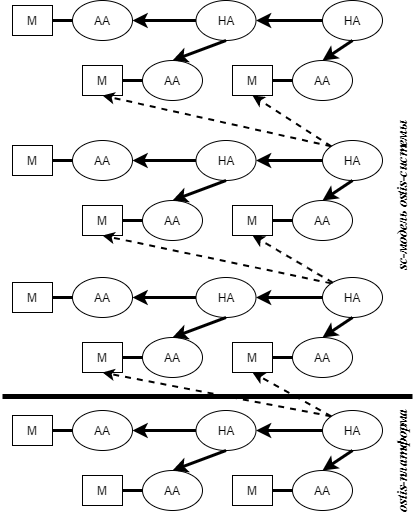
\includegraphics[scale=0.7]{images/part3/chapter_situation_management/agents-hierarchy.png}
	\label{fig:agents-hierarchy}
\end{figure}

Иерархический подход к описанию систем sc-агентов, определяющих операционную семантику \textit{решателей задач ostis-систем}, и соответственно, самих \textit{решателей задач ostis-систем} обладает рядом важных преимуществ, таких как обеспечение модифицируемости решателей и удобство их проектирования и отладки на разных уровнях.

Сказанное выше позволяет описать классификацию \textit{абстрактных sc-агентов} по признаку атомарности:

\begin{SCn}
	\scnheader{абстрактный sc-агент}
	\begin{scnrelfromset}{разбиение}
		\scnitem{неатомарный абстрактный sc-агент}
		\scnitem{атомарный абстрактный sc-агент}
	\end{scnrelfromset}
\end{SCn}

Под \textbf{\textit{неатомарным абстрактным sc-агентом}} понимается \textit{абстрактный sc-агент}, который декомпозируется на коллектив более простых \textit{абстрактных sc-агентов}, каждый из которых в свою очередь может быть как \textit{атомарным абстрактным sc-агентом}, так и \textbf{\textit{неатомарным абстрактным sc-агентом}}. При этом в каком либо варианте \textit{декомпозиции абстрактного sc-агента*} дочерний \textbf{\textit{неатомарный абстрактный sc-агент}} может стать \textit{атомарным абстрактным sc-агентом}, и реализовываться соответствующим образом.

Под \textbf{\textit{атомарным абстрактным sc-агентом}} понимается \textit{абстрактный sc-агент}, для которого уточняется способ его реализации, то есть существует соответствующая связка отношения \textit{программа sc-агента*}. Подчеркнем при этом, что в рамках конкретной \textit{ostis-системы} для каждого \textit{языка представления методов} может существовать своя иерархия \textit{абстрактных sc-агентов}.

В свою очередь, \textit{Язык SCP} позволяет установить границу между логико-семантической моделью \textit{ostis-системы} и \textit{ostis-платформой}. В связи с этим будем считать платформенно-независимыми \textit{абстрактные sc-агенты}, реализованные на \textit{Языке SCP} или более высокоуровневых языках на его основе, а платформенно-зависимыми \textit{абстрактные sc-агенты}, которые реализованы на уровне \textit{ostis-платформы} (например, с целью повышения их производительности). В то же время существует ряд \textit{абстрактных sc-агентов}, которые принципиально не могут быть реализованы на \textit{Языке SCP}. Сказанное отражено в следующей иерархии:

\begin{SCn}
\scnheader{абстрактный sc-агент}
\begin{scnrelfromset}{разбиение}
	\scnitem{внутренний абстрактный sc-агент}
	\scnitem{эффекторный абстрактный sc-агент}
	\scnitem{рецепторный абстрактный sc-агент}
\end{scnrelfromset}
\begin{scnrelfromset}{разбиение}
	\scnitem{абстрактный sc-агент, не реализуемый на Языке SCP}
	\scnitem{абстрактный sc-агент, реализуемый на Языке SCP}
\end{scnrelfromset}
\begin{scnrelfromset}{разбиение}
	\scnitem{абстрактный sc-агент интерпретации scp-программ}
	\scnitem{абстрактный программный sc-агент}
	\scnitem{абстрактный sc-метаагент}
\end{scnrelfromset}

\begin{scnrelfromset}{разбиение}	
	\scnitem{платформенно-зависимый абстрактный sc-агент}
	\begin{scnindent}
		\scnsuperset{абстрактный sc-агент, не реализуемый на Языке SCP}
	\end{scnindent}
	\scnitem{платформенно-независимый абстрактный sc-агент}
\end{scnrelfromset}

\scnheader{абстрактный sc-агент}
\begin{scnrelfromset}{разбиение}
	\scnitem{абстрактный sc-агент, не реализуемый на Языке SCP}
	\scnitem{абстрактный sc-агент, реализуемый на Языке SCP}
\end{scnrelfromset}
\begin{scnrelfromset}{разбиение}	
	\scnitem{платформенно-зависимый абстрактный sc-агент}
	\begin{scnindent}
		\scnsuperset{абстрактный sc-агент, не реализуемый на Языке SCP}
	\end{scnindent}
	\scnitem{платформенно-независимый абстрактный sc-агент}
\end{scnrelfromset}

\scnheader{абстрактный sc-агент, не реализуемый на Языке SCP}
\scnidtf{абстрактный sc-агент, который не может быть реализован на платформенно-независимом уровне}
\begin{scnrelfromset}{разбиение}
	\scnitem{эффекторный абстрактный sc-агент}
	\scnitem{рецепторный абстрактный sc-агент}
	\scnitem{абстрактный sc-агент интерпретации scp-программ}
\end{scnrelfromset}

\scnheader{абстрактный sc-агент, реализуемый на Языке SCP}
\scnidtf{абстрактный sc-агент, который может быть реализован на платформенно-независимом уровне}
\begin{scnrelfromset}{разбиение}
	\scnitem{абстрактный sc-метаагент}
	\scnitem{абстрактный программный sc-агент, реализуемый на Языке SCP}
\end{scnrelfromset}

\scnheader{абстрактный программный sc-агент}
\begin{scnrelfromset}{разбиение}
	\scnitem{эффекторный абстрактный sc-агент}
	\scnitem{рецепторный абстрактный sc-агент}
	\scnitem{абстрактный программный sc-агент, реализуемый на Языке SCP}
\end{scnrelfromset}	

\scnheader{атомарный абстрактный sc-агент}
\begin{scnrelfromset}{разбиение}
	\scnitem{платформенно-независимый абстрактный sc-агент}
	\scnitem{платформенно-зависимый абстрактный sc-агент}
\end{scnrelfromset}	
\end{SCn}

К \textbf{\textit{платформенно-независимым абстрактным \mbox{sc-агентам}}} относят \textit{атомарные абстрактные sc-агенты}, реализованные на базовом языке программирования \textit{Технологии OSTIS}, то есть на \textit{Языке SCP}.

При описании \textbf{\textit{платформенно-независимых абстрактных sc-агентов}} под \textit{платформенной независимостью} понимается платформенная независимость с точки зрения \textit{Технологии OSTIS}, то есть реализация на специализированном \textit{языке программирования}, ориентированном на обработку семантических сетей (\textit{Языке SCP}), поскольку \textit{атомарные sc-агенты}, реализованные на указанном языке могут свободно переноситься с одной \textit{ostis-платформы} на другую. При этом языки программирования, традиционно считающиеся платформенно-независимыми, в данном случае не могут считаться таковыми.

Существуют \textit{sc-агенты}, которые принципиально не могут быть реализованы на платформенно-независимом уровне, например, собственно \textit{sc-агенты} интерпретации \textit{sc-моделей} или рецепторные и эффекторные \textit{sc-агенты}, обеспечивающие взаимодействие с внешней средой.

К \textbf{\textit{платформенно-зависимым абстрактным sc-агентам}} относят \textit{атомарные абстрактные sc-агенты}, реализованные ниже уровня sc-моделей, то есть не на \textit{Языке SCP}, а на каком-либо другом языке описания \textit{программ}.

Каждый \textbf{\textit{внутренний абстрактный sc-агент}} обозначает класс \textit{sc-агентов}, которые реагируют на события в \textit{sc-памяти} и осуществляют преобразования исключительно в рамках этой же \textit{sc-памяти}.

Каждый \textbf{\textit{эффекторный абстрактный sc-агент}} обозначает класс \textit{sc-агентов}, которые реагируют на события в \textit{sc-памяти} и осуществляют преобразования во внешней относительно данной \textit{ostis-системы} среде.

Каждый \textbf{\textit{рецепторный абстрактный sc-агент}} обозначает класс \textit{sc-агентов}, которые реагируют на события во внешней относительно данной \textit{ostis-системы} среде и осуществляют преобразования в памяти данной системы.

Каждый \textbf{\textit{абстрактный sc-агент, не реализуемый на Языке SCP}} должен быть реализован на уровне \textit{ostis-платформы}, в том числе, аппаратной. К таким \textit{абстрактным sc-агентам} относятся \textit{абстрактные sc-агенты интерпретации scp-программ}, а также \textit{эффекторные} и \textit{рецепторные абстрактные sc-агенты}.

Каждый \textbf{\textit{абстрактный sc-агент, реализуемый на Языке SCP}} может быть реализован на \textit{Языке SCP}, то есть платформенно-независимом уровне, но при необходимости, может реализовываться и на уровне \textit{ostis-платформы}, например, с целью повышения производительности.

К \textbf{\textit{абстрактным sc-агентам интерпретации scp-программ}} относятся не реализуемые на платформенно-независимом уровне \textit{абстрактные sc-агенты}, обеспечивающие интерпретацию \textit{scp-программ} и \textit{\mbox{scp-метапрограмм}}, в том числе создание \textit{scp-процессов}, собственно интерпретацию \textit{scp-операторов}, а также другие вспомогательные действия. По сути, агенты данного класса обеспечивают работу sc-агентов более высоких уровней (\textit{программных sc-агентов} и \textit{sc-метаагентов}), реализованных\textit{ на Языке SCP}, в частности, обеспечивают соблюдение указанными \textit{агентами} общих принципов синхронизации.

К \textbf{\textit{абстрактным программным sc-агентам}} относятся все \textit{абстрактные sc-агенты}, обеспечивающие основной функционал системы, то есть ее возможность решать те или иные задачи. Агенты данного класса должны работать в соответствии с общими принципами синхронизации деятельности субъектов в sc-памяти.

Задачей \textbf{\textit{абстрактных sc-метаагентов}} является координация деятельности \textit{абстрактных программных sc-агентов}, в частности, решение проблемы взаимоблокировок. Агенты данного класса могут быть реализованы на \textit{Языке SCP}, однако для синхронизации их деятельности используются другие принципы, соответственно, для реализации таких агентов требуется Язык SCP другого уровня, типология операторов которого полностью аналогична типологии scp-операторов, однако эти операторы имеют другую операционную семантику, учитывающую отличия в принципах синхронизации (работы с \textit{блокировками*}). Программы такого языка будем называть \textit{scp-метапрограммами}, соответствующие им \mbox{\textit{процессы в sc-памяти} -- \textit{scp-метапроцессами}}, операторы -- \textit{scp-метаоператорами}.

\begin{SCn}
\scnheader{декомпозиция абстрактного sc-агента*}
\scniselement{отношение декомпозиции}
\scnrelfrom{первый домен}{неатомарный абстрактный sc-агент}
\end{SCn}

Отношение \textbf{\textit{декомпозиции абстрактного sc-агента*}} трактует \textit{неатомарные абстрактные sc-агенты} как коллективы более простых \textit{абстрактных sc-агентов}, взаимодействующих через \textit{sc-память}.
	
Другими словами, \textbf{\textit{декомпозиция абстрактного sc-агента*}} на \textit{абстрактные sc-агенты} более низкого уровня уточняет один из возможных подходов к реализации этого \textit{абстрактного sc-агента} путем построения коллектива более простых \textit{абстрактных sc-агентов}.

\begin{SCn}
\scnheader{sc-агент}
\scnidtf{агент над sc-памятью}
\scnsubset{субъект}
\scnrelfrom{семейство подмножеств}{абстрактный sc-агент}
\end{SCn}

Под \textbf{\textit{sc-агентом}} понимается конкретный экземпляр (с теоретико-множественной точки зрения - элемент) некоторого \textit{атомарного абстрактного sc-агента}, работающий в какой-либо конкретной интеллектуальной системе.
	
Таким образом, каждый \textit{sc-агент} - это субъект, способный выполнять некоторый класс однотипных действий либо только над \textit{sc-памятью}, либо над sc-памятью и внешней средой (для эффекторных \textit{sc-агентов}). Каждое такое действие инициируется либо состоянием или ситуацией в sc-памяти, либо состоянием или ситуацией во внешней среде (для рецепторных sc-агентов-датчиков),  соответствующей условию инициирования \textit{атомарного абстрактного sc-агента}, экземпляром которого является заданный \textit{sc-агент}. В данном случае можно провести аналогию между принципами объектно-ориентированного программирования, рассматривая \textit{атомарный абстрактный sc-агент} как класс, а конкретный \textit{sc-агент} --- как экземпляр, конкретную имплементацию этого класса.
	
Взаимодействие \textit{sc-агентов} осуществляется только через \textit{sc-память}. Как следствие, результатом работы любого \textit{sc-агента} является некоторое изменение состояния \textit{sc-памяти}, то есть удаление либо генерация каких-либо \textit{sc-элементов}.
	
В общем случае один \textit{sc-агент} может явно передать управление другому \textit{sc-агенту}, если этот \textit{sc-агент} априори известен. Для этого каждый \textit{sc-агент} в \textit{sc-памяти} имеет обозначающий его \textit{sc-узел}, с которым можно связать конкретную ситуацию в текущем состоянии \textit{базы знаний}, которую инициируемый \textit{sc-агент} должен обработать.
	
Однако далеко не всегда легко определить того \textit{sc-агента}, который должен принять управление от заданного \textit{sc-агента}, в связи с чем описанная выше ситуация возникает крайне редко. Более того, иногда условие инициирования \textit{sc-агента} является результатом деятельности непредсказуемой группы \textit{sc-агентов}, равно как и одна и та же конструкция может являться условием инициирования целой группы \textit{sc-агентов}.

При этом общаются через \textit{sc-память} не \textit{программы sc-агентов*}, а сами описываемые данными программами \textit{sc-агенты}.

В процессе работы \textit{sc-агент} может сам для себя порождать вспомогательные \textit{sc-элементы}, которые сам же удаляет после завершения акта своей деятельности (это вспомогательные \textit{структуры}, которые используются в качестве "информационных лесов"{} только в ходе выполнения соответствующего акта деятельности и после завершения этого акта удаляются).

\begin{SCn}
\scnheader{sc-агент}
\scnsuperset{активный sc-агент}
\begin{scnrelfromlist}{первый домен}
	\scnitem{ключевые sc-элементы sc-агента*}
	\scnitem{программа sc-агента*}	
	\scnitem{первичное условие инициирования*}
	\scnitem{условие инициирования и результат*}
\end{scnrelfromlist}
\end{SCn}

Под \textbf{\textit{активным sc-агентом}} понимается \textit{sc-агент} ostis-системы, который реагирует на события, соответствующие его условию инициирования, и, как следствие, его \textit{первичному условию инициирования*}. Не входящие во множество \textbf{\textit{активных sc-агентов}} \textit{sc-агенты} не реагируют ни на какие события в \textit{sc-памяти}.

Связки отношения \textbf{\textit{ключевые sc-элементы sc-агента*}} связывают между собой \textit{sc-узел}, обозначающий \textit{абстрактный sc-агент} и \textit{sc-узел}, обозначающий множество \textit{sc-элементов}, которые являются ключевыми для данного \textit{абстрактного sc-агента}, то данные \textit{sc-элементы} явно упоминаются в рамках программ, реализующих данный \textit{абстрактный sc-агент}.

Связки отношения \textbf{\textit{программа sc-агента*}} связывают между собой \textit{sc-узел}, обозначающий \textit{атомарный абстрактный sc-агент} и \textit{sc-узел}, обозначающий множество программ, реализующих указанный \textit{атомарный абстрактный sc-агент}. В случае \textit{платформенно-независимого абстрактного sc-агента} каждая связка отношения \textit{программа sc-агента*} связывает \textit{sc-узел}, обозначающий указанный \textit{абстрактный sc-агент} с множеством \textit{scp-программ}, описывающих деятельность данного \textit{абстрактного sc-агента}. Данное множество содержит одну \textit{агентную scp-программу}, и произвольное количество (может быть, и ни одной) \textit{scp-программ}, которые необходимы для выполнения указанной \textit{агентной scp-программы}.
	
В случае \textit{платформенно-зависимого абстрактного sc-агента} каждая связка отношения \textit{программа \mbox{sc-агента*}} связывает \textit{sc-узел}, обозначающий указанный \textit{абстрактный sc-агент} с множеством файлов, содержащих исходные тексты программы на некотором внешнем языке программирования, реализующей деятельность данного \textit{абстрактного sc-агента}.

Связки отношения \textbf{\textit{первичное условие инициирования*}} связывают между собой \textit{sc-узел}, обозначающий \textit{абстрактный sc-агент} и бинарную ориентированную пару, описывающую первичное условие инициирования данного \textit{абстрактного sc-агента}, то есть такой спецификацию \textit{ситуации} в \textit{sc-памяти}, возникновение которой побуждает \textit{sc-агента} перейти в активное состояние и начать проверку наличия своего полного условия инициирования.
	
Первым компонентом данной ориентированной пары является знак некоторого класса \textit{элементарных событий в sc-памяти*}, например, \textit{событие добавления sc-дуги, выходящей из заданного sc-элемента*}.

Вторым компонентом данной ориентированной пары является произвольный в общем случае \textit{sc-элемент}, с которым непосредственно связан указанный тип события в \textit{sc-памяти}, то есть, например, \textit{sc-элемент}, из которого выходит либо в который входит генерируемая либо удаляемая \textit{sc-дуга}, либо \textit{файл}, содержимое которого было изменено.

После того, как в \textit{sc-памяти} происходит некоторое событие, активизируются все \textit{активные sc-агенты}, \textbf{\textit{первичное условие инициирования*}} которых соответствует произошедшему событию.

Связки отношения \textbf{\textit{условие инициирования и результат*}} связывают между собой \textit{sc-узел}, обозначающий \textit{абстрактный sc-агент} и бинарную ориентированную пару, связывающую условие инициирования данного \textit{абстрактного sc-агента} и результаты выполнения данного экземпляров данного \textit{sc-агента} в какой-либо конкретной системе.
	
Указанную ориентированную пару можно рассматривать как логическую связку импликации, при этом на \textit{sc-переменные}, присутствующие в обеих частях связки, неявно накладывается квантор всеобщности, на \textit{sc-переменные}, присутствующие либо только в посылке, либо только в заключении неявно накладывается квантор существования.

Первым компонентом указанной ориентированной пары является логическая формула, описывающая условие инициирования описываемого \textit{абстрактного sc-агента}, то есть конструкции, наличие которой в \textit{sc-памяти} побуждает \textit{sc-агент} начать работу по изменению состояния \textit{sc-памяти}. Данная логическая формула может быть как атомарной, так и неатомарной, в которой допускается использование любых связок логического языка.

Вторым компонентом указанной ориентированной пары является \textit{логическая формула}, описывающая возможные результаты выполнения описываемого абстрактного \textit{sc-агента}, то есть описание произведенных им изменений состояния \textit{sc-памяти}. Данная \textit{логическая формула} может быть как атомарной, так и неатомарной, в которой допускается использование любых связок \textit{логического языка}.

\begin{SCn}
\scnheader{описание поведения sc-агента}
\scnsubset{семантическая окрестность}
\end{SCn}

\textbf{\textit{описание поведения sc-агента}} представляет собой \textit{семантическую окрестность}, описывающую деятельность \textit{sc-агента} до какой-либо степени детализации, однако такое описание должно быть строгим, полным и однозначно понимаемым. Как любая другая \textit{семантическая окрестность}, \textbf{\textit{описание поведения sc-агента}} может быть протранслировано на какие-либо понятные, общепринятые средства, не требующие специального изучения, например на \textit{естественный язык}.

Описываемый \textit{абстрактный sc-агент} входит в соответствующее \textbf{\textit{описание поведения sc-агента}} под атрибутом \textit{ключевой sc-элемент\scnrolesign}.

\section{Принципы синхронизации деятельности sc-агентов}
\label{sec_ps_sync}

\begin{SCn}
\begin{scnrelfromlist}{ключевое понятие}
	\scnitem{действие в sc-памяти}
	\scnitem{блокировка*}
	\scnitem{тип блокировки}
	\scnitem{планируемая блокировка*}
	\scnitem{приоритет блокировки*}
	\scnitem{удаляемые sc-элементы*}
	\scnitem{транзакция в sc-памяти}	
\end{scnrelfromlist}
\end{SCn}

Одной из важных особенностей \textit{многоагентного подхода} к решению задач является возможность параллельного решения различных задач, что в свою очередь, предполагает параллельность выполнения соответствующих информационных процессов.

Понятия \textit{действие в sc-памяти}, и \textit{процесс в sc-памяти} (\textit{информационный процесс}, выполняемый агентом в семантической памяти), являются синонимичными, поскольку все процессы, протекающие в sc-памяти, являются осознанными и выполняются каким-либо \textit{sc-агентами}. Тем не менее, когда идет речь о синхронизации выполнения каких-либо преобразований в памяти компьютерной системы, в литературе принято использовать именно термины ``процесс'', ``взаимодействие процессов'' (см. \scncite{Dijkstra2002}, \scncite{Hoare1983}), в связи с чем будем использовать этот термин при описании принципов синхронизации деятельности sc-агентов при выполнении ими параллельных \textit{процессов в sc-памяти}.

\begin{SCn}
\scnheader{действие в sc-памяти}
\scnidtftext{часто используемый sc-идентификатор}{\textbf{\textit{процесс в sc-памяти}}}
	
\scnheader{процесс в sc-памяти}
\begin{scnrelfromset}{разбиение}
	\scnitem{процесс в sc-памяти, соответствующий платформенно-зависимому sc-агенту}
	\scnitem{scp-процесс}	
	\begin{scnindent}
	\begin{scnrelfromset}{разбиение}
		\scnitem{scp-процесс, не являющийся scp-метапроцессом}
		\scnitem{scp-метапроцесс}	
	\end{scnrelfromset}
	\end{scnindent}
\end{scnrelfromset}

\scnheader{процесс в sc-памяти, соответствующий платформенно-зависимому sc-агенту}
	\begin{scnrelfromset}{разбиение}
	\scnitem{процесс в sc-памяти, соответствующий платформенно-зависимому sc-агенту и не являющийся действием абстрактной scp-машины}
	\scnitem{действие абстрактной scp-машины}	
	\begin{scnindent}
		\scnsuperset{действие интерпретации scp-программы}
	\end{scnindent}
\end{scnrelfromset}
\end{SCn}

Для синхронизации выполнения \textit{процессов в sc-памяти} предлагается использовать механизм блокировок, построенный на основе существующих алгоритмов синхронизации информационных процессов в традиционных системах (см. \scncite{Dijkstra2002}, \scncite{Hoare1983}). В качестве возможного направления развития данного подхода можно указать набирающие популярность идеи lock-free алгоритмов (см. \scncite{Chatterjee2022}).

Отношение \textbf{\textit{блокировка*}} связывает знаки \textit{действий в sc-памяти} со знаками \textit{структур} (ситуативных), которые содержат элементы, заблокированные на время выполнения данного действия или на какую-то часть этого периода. Каждая такая \textit{структура} принадлежит какому-либо из \textit{типов блокировки}.

Первым компонентом связок отношения \textbf{\textit{блокировка*}} является знак \textit{действия в sc-памяти}, вторым --- знак заблокированной \textit{структуры}.

\begin{SCn}	
\scnheader{блокировка*}
\scniselement{бинарное отношение}

\scnheader{тип блокировки}
\scnhaselement{полная блокировка}
\scnhaselement{блокировка на любое изменение}
\scnhaselement{блокировка на удаление}
\end{SCn}	

\begin{figure}[H]
	\caption{SCg-текст. Пример использования блокировок}
	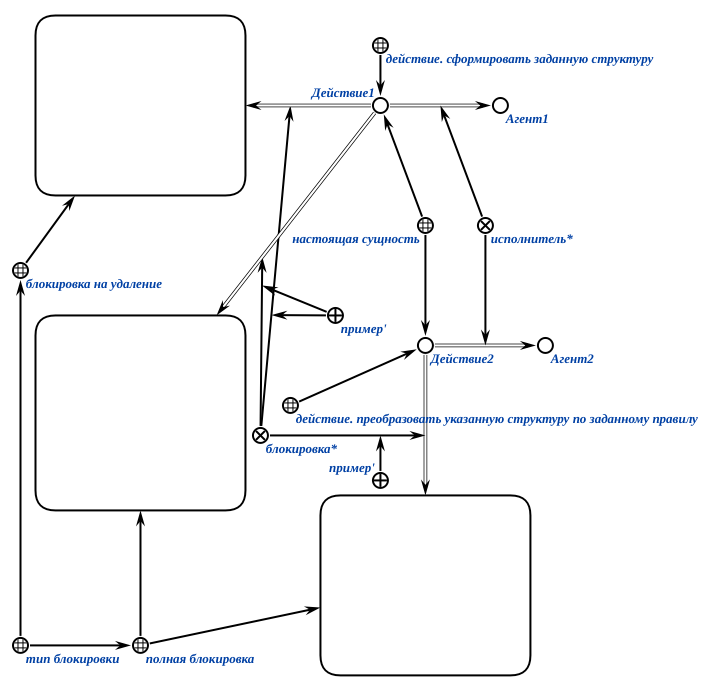
\includegraphics[scale=0.8]{images/part3/chapter_situation_management/lock.png}
	\label{fig:lock}
\end{figure}

Множество \textbf{\textit{тип блокировки}} содержит все возможные классы блокировок, то есть \textit{структуры}, содержащие \textit{sc-элементы}, заблокированные каким-либо \textit{sc-агентом} на время выполнения им некоторого \textit{действия в sc-памяти}.

Каждая \textit{структура}, принадлежащая множеству \textbf{\textit{полная блокировка}} содержит \textit{sc-элементы}, просмотр и изменение (удаление, добавление инцидентных \textit{sc-коннекторов}, удаление самих \textit{sc-элементов}, изменение содержимого в случае файла) которых запрещены всем \textit{sc-агентам}, кроме собственно \textit{sc-агента}, выполняющего соответствующее данной структуре \textit{действие в sc-памяти}, связанное с ней отношением \textit{блокировка*}.
	
Для того, чтобы исключить возможность реализации \textit{sc-агентов}, которые могут внести изменения в конструкции, описывающие блокировки других \textit{sc-агентов}, все элементы этих конструкций, в том числе, сам знак \textit{структуры}, содержащей заблокированные \textit{sc-элементы} (принадлежащей как множеству \textbf{\textit{полная блокировка}}, так и любому другому \textit{типу блокировки}) и связки отношения \textit{блокировка*}, связывающие эту \textit{структуру} и конкретное \textit{действие в sc-памяти}, добавляются в \textbf{\textit{полную блокировку}}, соответствующую данному \textit{действию в sc-памяти}. Таким образом, каждой \textbf{\textit{полной блокировке}} соответствует петля принадлежности, связывающая ее знак с самим собой.

Каждая \textit{структура}, принадлежащая множеству \textbf{\textit{блокировка на любое изменение}} содержит \textit{sc-элементы}, изменение (физическое удаление, добавление инцидентных \textit{sc-коннекторов}, физическое удаление самих \textit{\mbox{sc-элементов}}, изменение содержимого в случае файла) которых запрещено всем \textit{sc-агентам}, кроме собственно \textit{sc-агента}, выполняющего соответствующее данной структуре \textit{действие в sc-памяти}, связанное с ней отношением \textit{блокировка*}. Однако не запрещен просмотр (чтение) этих \textit{sc-элементов} любым \textit{sc-агентом}.

Каждая \textit{структура}, принадлежащая множеству \textbf{\textit{блокировка на удаление}} содержит \textit{sc-элементы}, удаление которых запрещено всем \textit{sc-агентам}, кроме собственно \textit{sc-агента}, выполняющего соответствующее данной структуре \textit{действие в sc-памяти}, связанное с ней отношением \textit{блокировка*}. Однако не запрещен просмотр (чтение) этих \textit{sc-элементов} любым \textit{sc-агентом}, добавление инцидентных sc-коннекторов.

Рассмотрим принципы работы с блокировками:

\begin{textitemize}
	\item в каждый момент времени одному \textit{процессу в sc-памяти} может соответствовать только одна блокировка каждого типа;
	\item в каждый момент времени одному \textit{процессу в sc-памяти} может соответствовать только одна блокировка, установленная на некоторый конкретный sc-элемент;
	\item при завершении выполнения любого \textit{процесса в sc-памяти} все установленные им блокировки автоматически снимаются;
	\item для повышения эффективности работы системы в целом каждый процесс должен в каждый момент времени блокировать минимально необходимое множество sc-элементов, снимая блокировку с каждого sc-элемента сразу же, как это становится возможным (безопасным);
	\item В случае когда в рамках \textit{процесса в sc-памяти} явно выделяются более частные подпроцессы (при помощи отношений \textit{темпоральная часть*, поддействие*, декомпозиция действия*} и так далее), то каждый такой подпроцесс с точки зрения синхронизации выполнения рассматривается как самостоятельный процесс, которому в соответствие могут быть поставлены все необходимые блокировки.
	\begin{textitemize}
		\item все дочерние процессы в sc-памяти имеют доступ к блокировкам родительского процесса так же, как если бы это были блокировки соответствующие каждому из таких дочерних процессов;
		\item в свою очередь, родительский процесс не имеет какого-либо привилегированного доступа к sc-элементам, заблокированным дочерними процессами, и работает с ними так же, как любой другой процесс в sc-памяти. Исключение составляют sc-элементы, обозначающие сами дочерние процессы, поскольку родительский процесс должен иметь возможность управления дочерним, например, приостановки или прекращения их выполнения;
		\item все дочерние процессы по отношению друг к другу работают так же, как и по отношению к любым другим процессам;
		\item в случае, когда родительский процесс приостанавливает выполнение (становится \textit{отложенным действием}), \uline{все} его дочерние процессы также приостанавливают выполнение. В свою очередь, приостановка одного из дочерних процессов в общем случае не инициирует явно остановку всего родительского процесса и соответственно других дочерних.
		\end{textitemize}
\end{textitemize}

Рассмотрим принципы работы с \textit{полными блокировками}:
\begin{textitemize}
	\item если sc-элемент, инцидентный некоторому sc-коннектору, попадает в какую-либо полную блокировку, то сам этот sc-коннектор по умолчанию также считается заблокированным этой же блокировкой. Обратное в общем случае неверно, так как часть sc-коннекторов, инцидентных некоторому sc-элементу, может быть полностью заблокирована, при этом сам этот элемент заблокирован не будет. Такая ситуация типична, например, для sc-узлов, обозначающих классы понятий;
	\item каждый процесс в sc-памяти может свободно изменять или удалять любые sc-элементы, попадающие в полную блокировку, соответствующую этому процессу.
\end{textitemize}

Принципы работы с \textit{полными блокировками}, с одной стороны, наиболее просты, поскольку все процессы, кроме установившего такую блокировку, не имеют доступа к заблокированным \mbox{sc-элементам} и конфликты возникнуть не могут. С другой стороны, частое использование блокировок такого типа может привести к тому, что система не сможет использовать в полной мере имеющиеся у нее знания и давать неполные или даже некорректные ответы на поставленные вопросы.

Рассмотрим принципы работы с \textit{блокировками на любое изменение} и \textit{блокировками на удаление}:
\begin{textitemize}
	\item на один и тот же sc-элемент в один момент времени может быть установлена только одна блокировка одного типа, но разные процессы могут одновременно установить на один и тот же элемент блокировки двух разных типов. Это касается случая, когда первый процесс установил на некоторый sc-элемент блокировку на удаление, а второй процесс затем устанавливает блокировку на любое изменение. В других случаях возникает конфликт блокировок;
	\item установка блокировки любого типа также считается изменением, таким образом, если на некоторый \mbox{sc-элемент} была установлена блокировка на любое изменение, то другой процесс не сможет установить на этот же sc-элемент блокировку любого типа, пока первый процесс не снимет свою;
	\item если блокировка на удаление устанавливается на некоторый sc-коннектор, то по умолчанию та же блокировка устанавливается на инцидентные этому sc-коннектору sc-элементы, поскольку удаление этих элементов приведет к удалению этого коннектора.
\end{textitemize}

\begin{SCn}
\scnheader{процесс в sc-памяти}
\scnrelfrom{разбиение}{Классификация процессов в sc-памяти с точки зрения синхронизации их выполнения}
\begin{scnindent}
\begin{scneqtoset}
	\scnitem{действие поиска sc-элементов}
	\scnitem{действие генерации sc-элементов}
	\scnitem{действие удаления sc-элементов}
	\scnitem{действие установки блокировки некоторого типа на некоторый sc-элемент}
	\scnitem{действие снятия блокировки с некоторого sc-элемента}
\end{scneqtoset}
\end{scnindent}
\end{SCn}

В некоторых случаях для того, чтобы обеспечить синхронизацию, необходимо объединять несколько элементарных действий над sc-памятью в одно неделимое действие (\textbf{\textit{транзакцию в sc-памяти}}), для которого гарантируется, что ни один сторонний процесс не сможет прочитать или изменить участвующие в этом действии sc-элементы, пока действие не завершится. При этом, в отличие от ситуации с полной блокировкой, процесс, пытающийся получить доступ к таким элементам, не продолжает выполнение так, как если бы этих элементов просто не было в sc-памяти, а ожидает завершения транзакции, после чего может выполнять с данными элементами любые действия согласно общим принципам синхронизации процессов. Проблема обеспечения транзакций не может быть решена на уровне SC-кода и требует реализации таких неделимых действий на уровне \textit{ostis-платформы}.

В случае выполнения \textit{действия поиска sc-элементов} все найденные и сохраненные в рамках какого-либо процесса sc-элементы попадают в соответствующую данному процессу \textit{блокировку на любое изменение}. Таким образом, гарантируется целостность фрагмента базы знаний, с которым работает некоторый процесс в sc-памяти. При этом поиск и автоматическая установка такой блокировки должны быть реализованы как \textit{транзакция в sc-памяти}.
	
Такой подход также позволяет избежать ситуации, когда один процесс заблокировал некоторый sc-элемент на любое изменение, а второй процесс пытается сгенерировать или удалить \textit{sc-коннектор}, инцидентный данному \textit{sc-элементу}. В таком случае второй процесс должен будет предварительно найти и заблокировать указанный \textit{sc-элемент} на любое изменение, что вызовет конфликт блокировок (\textit{взаимоблокировку*}).

В случае генерации любого sc-элемента в рамках некоторого процесса он автоматически попадает в полную блокировку, соответствующую данному процессу. При этом генерация и автоматическая установка такой блокировки должны быть реализованы как \textit{транзакция в sc-памяти}. При необходимости сгенерированные элементы могут быть удалены (то есть их временное существование вообще никак не отразится на деятельности других процессов) или разблокированы в случае, когда сгенерирована информация, которая может иметь некоторую ценность в дальнейшем.

В случае если какой-либо процесс пытается установить блокировку любого типа на какой-либо sc-элемент, уже заблокированный каким-либо другим процессом, то, с одной стороны, блокировка не может быть установлена, пока другой процесс не разблокирует указанный sc-элемент; с другой стороны, для того чтобы обеспечить возможность поиска и устранения \textit{взаимоблокировок}, необходимо явно указывать тот факт, что какой-либо процесс хочет получить доступ к какому-либо заблокированному другим процессом sc-элементу. Для того чтобы иметь возможность указать, какие процессы пытаются заблокировать уже заблокированный \textit{sc-элемент}, предлагается наряду с отношением \textit{блокировка*} использовать отношение \textit{планируемая блокировка*}, полностью аналогичное отношению \textit{блокировка*}.
	
Описанный механизм регулирует также и процессы поиска, поскольку поиск и сохранение некоторого sc-элемента предполагает установку \textit{блокировки на любое изменение}. Кроме того, следует учитывать, что на один sc-элемент \textit{блокировка на любое изменение} может быть установлена после \textit{блокировки на удаление}, соответствующей другому процессу. В этом случае использовать отношение \textit{планируемые блокировки*} нет необходимости.
	
Действие проверки наличия на некотором sc-элементе блокировки и в зависимости от результата проверки, установки блокировки или планируемой блокировки (с указанием приоритета при необходимости) должно быть реализовано как транзакция.

\begin{SCn}
\scnheader{планируемая блокировка*}
\scnsubset{блокировка*}
\end{SCn}

Процесс, которому в соответствие поставлена \textit{планируемая блокировка*}, приостанавливает выполнение до тех пор, пока уже установленные блокировки не будут сняты, после чего \textit{планируемая блокировка*} становится реальной \textit{блокировкой*} и процесс продолжает выполнение в соответствии с общими правилами.

\begin{SCn}
\scnheader{приоритет блокировки*}
\scnrelfrom{область определения}{планируемая блокировка*}
\end{SCn}

В случае, когда на один и тот же sc-элемент планируют установить блокировку сразу несколько процессов, используется отношение \textit{приоритет блокировки*}, связывающее между собой пары отношения \textit{планируемая блокировка*}. Как правило, приоритет блокировки определяется тем, какой из процессов раньше попытался установить блокировку на рассматриваемый sc-элемент, хотя в общем случае приоритет может устанавливаться или меняться в зависимости от дополнительных критериев.

В случае попытки удаления некоторого sc-элемента некоторым процессом удаление может быть осуществлено только в случае, когда на данный sc-элемент не установлена (и не планируется) ни одна блокировка каким-либо другим процессом.
	
В других случаях необходимо обеспечить корректное завершение выполнения всех процессов, работающих с данным sc-элементом, и только потом удалить его физически.
	
Для реализации такой возможности каждому процессу в соответствие может быть поставлено множество удаляемых данным процессом sc-элементов.

Действие проверки наличия блокировок или планируемых блокировок на удаляемый sc-элемент и собственно его удаление или добавление во множество удаляемых sc-элементов для соответствующего процесса должно быть реализовано как транзакция.

\begin{SCn}
\scnheader{удаляемые sc-элементы*}
\scnrelfrom{первый домен}{процесс в sc-памяти}
\end{SCn}

sc-элементы, попавшие во множество удаляемых sc-элементов некоторого процесса в sc-памяти, доступны процессам, уже установившим (или планирующим установить) на эти sc-элементы блокировки ранее (до попытки его удаления), а для всех остальных процессов эти sc-элементы уже считаются удаленными. Процесс, пытающийся удалить sc-элемент, приостанавливает свое выполнение до того момента, пока все заблокировавшие и планирующие заблокировать данный sc-элемент процессы не разблокируют его. В общем случае один sc-элемент может входить во множества удаляемых элементов одновременно для нескольких процессов, в этом случае все такие процессы одновременно продолжат выполнение после снятия с этого sc-элемента всех блокировок. Если удаление пытается осуществить один из процессов, уже установивший на указанный sc-элемент блокировку, то алгоритм действий остается прежним --- sc-элемент добавляется во множество удаляемых данным процессом sc-элементов, и будет физически удален, как только все остальные процессы, установившие на данный sc-элемент блокировки, снимут их.

Рассмотрим алгоритм снятия блокировки с некоторого sc-элемента:
\begin{textitemize}
	\item если на данный sc-элемент установлена одна или несколько \textit{планируемых блокировок*}, то первая из них по приоритету (или единственная) становится \textit{блокировкой*}, соответствующий ей процесс продолжает выполнение (становится настоящей сущностью); связка отношения приоритет выполнения, соответствовавшая удаленной связке отношения \textit{планируемая блокировка*} также удаляется, то есть приоритет смещается на одну позицию;
	\item если \textit{планируемых блокировок*}, установленных на данный sc-элемент, нет, но он попадает во множество удаляемых sc-элементов для одного или нескольких процессов, то рассматриваемый sc-элемент физически удаляется, а приостановленные до его удаления процессы продолжают свое выполнение (становится настоящими сущностями);
	\item если на данный sc-элемент не установлены планируемые блокировки и он не входит во множество удаляемых для какого-либо процесса, то блокировка просто снимается без каких-либо дополнительных изменений.
\end{textitemize}

\begin{SCn}
\scnheader{транзакция в sc-памяти}
\begin{scnrelfromset}{разбиение}
	\scnitem{поиск некоторой конструкции в sc-памяти и автоматическая установка блокировки на любое изменение на найденные sc-элементы}
	\scnitem{генерация некоторого sc-элемента и автоматическая установка на него полной блокировки}
	\scnitem{проверка наличия на некотором sc-элементе блокировки и в зависимости от результата проверки установка блокировки или планируемой блокировки}	
	\scnitem{проверка наличия блокировок или планируемых блокировок на удаляемый sc-элемент и собственно его удаление или добавление во множество удаляемых sc-элементов для соответствующего процесса}	
	\scnitem{снятие блокировки с заданного sc-элемента и при необходимости установка первой по приоритету планируемой блокировки или удаление данного sc-элемента, если он входит во множество удаляемых sc-элементов для некоторого процесса}	
	\scnitem{поиск подпроцессов процесса и добавление их во множество отложенных действий в случае добавления самого процесса в данное множество}	
	\scnitem{поиск подпроцессов процесса и удаление их из множества отложенных действий в случае удаления самого процесса из данного множества}	
\end{scnrelfromset}
\end{SCn}

При реализации \textit{абстрактных программных sc-агентов} на \textit{Языке SCP}, соблюдение всех принципов синхронизации соответствующих этим sc-агентам процессов обеспечивается на уровне \textit{sc-агентов интерпретации scp-программ}, то есть средствами \textit{ostis-платформы}. При реализации \textit{абстрактных программных sc-агентов} на уровне \textit{ostis-платформы}, соблюдение всех принципов синхронизации возлагается, во-первых, непосредственно на разработчика агентов, во-вторых, --- на разработчика \textit{ostis-платформы}. Так, например, платформа может предоставлять доступ к хранимым в sc-памяти элементам через некоторый \textit{программный интерфейс}, уже учитывающий принципы работы с блокировками, что избавит разработчика агентов от необходимости учитывать все эти принципы вручную.

Кроме того, выделяется ряд специфичных принципов работы \textit{абстрактных программных sc-агентов}, реализованных на \textit{Языке SCP}:
\begin{textitemize}
\item в результате появления в sc-памяти некоторой конструкции, удовлетворяющей условию инициирования какого-либо \textit{абстрактного sc-агента}, реализованного при помощи \textit{Языка SCP}, в \textit{sc-памяти} генерируется и инициируется \textit{scp-процесс}. В качестве шаблона для генерации используется \textit{агентная scp-программа}, соответствующая данному \textit{абстрактному sc-агенту}.
\item каждый такой \textit{scp-процесс}, соответствующий некоторой \textit{агентной \mbox{scp-программе}}, может быть связан с набором структур, описывающих блокировки различных типов. Таким образом, синхронизация взаимодействия параллельно выполняемых \textit{scp-процесcов} осуществляется так же, как и в случае любых других \textit{действий в sc-памяти}.
\item несмотря на то что каждый \textit{scp-оператор} представляет собой атомарное действие в sc-памяти, являющееся поддействием в рамках всего \textit{\mbox{scp-процесса}}, блокировки, соответствующие одному оператору, не вводятся, чтобы избежать громоздкости и избытка дополнительных системных конструкций, создаваемых при выполнении некоторого \textit{scp-процесса}. Вместо этого используются блокировки, общие для всего \textit{scp-процесса}. Таким образом, \textit{агенты интерпретации scp-программ} работают только с учетом блокировок, общих для всего интерпретируемого \textit{scp-процесса}.
\item процессы, описывающие деятельность агентов интерпретации \textit{scp-программ}, как правило, не создаются, следовательно, и не вводятся соответствующие им блокировки. Поскольку такие агенты работают с уникальным scp-процессом и их число ограничено и известно, то использование блокировок для их синхронизации не требуется.
\item в случае приостановки \textit{scp-процесса} (добавления его во множество \textit{отложенных действий}) в соответствии с общими правилами синхронизации все его дочерние процессы также должны быть	приостановлены. В связи с этим все \textit{scp-операторы}, которые в	этот момент являются \textit{настоящими сущностями}, становятся	\textit{отложенными действиями}.
\item во избежание нежелательных изменений в самом теле \textit{scp-процесса}, вся конструкция, сгенерированная на основе некоторой \textit{scp-программы} (весь \textit{sc-текст}, описывающий декомпозицию \textit{scp-процесса} на \textit{scp-операторы}), должна быть добавлена в \textit{полную блокировку}, соответствующую данному \textit{scp-процессу}.
\item при необходимости разблокировать или заблокировать некоторую конструкцию каким-либо типом блокировки используются соответствующие \textit{scp-операторы} класса \textit{scp-оператор управления блокировками}.
\item после завершения выполнения некоторого scp-процесса его текст, как правило, удаляется из \textit{sc-памяти}, а все заблокированные конструкции освобождаются (разрушаются знаки структур, обозначавших блокировки).
\item как правило, частный \textit{класс действий}, соответствующий конкретной \textit{scp-программе}, явно не вводится, а используется более общий класс \textit{scp-процесс}, за исключением тех случаев, когда введение	специального \textit{класса действий} необходимо по каким-либо другим соображениям.
\end{textitemize}

В общем случае весь механизм блокировок может описываться как на уровне \textit{SC-кода} (для повышения уровня \textit{платформенной независимости}), так и при необходимости может быть реализован на уровне \textit{ostis-платформы}, например для повышения производительности. Для этого каждому выполняемому в sc-памяти процессу на нижнем уровне может быть поставлена в соответствие некая уникальная таблица, в каждый момент времени содержащая перечень заблокированных элементов с указанием типа блокировки.

Рассмотрим пример применения описанного механизма.

\begin{figure}[H]
	\caption{SCg-текст. Пример использования планируемых блокировок}
	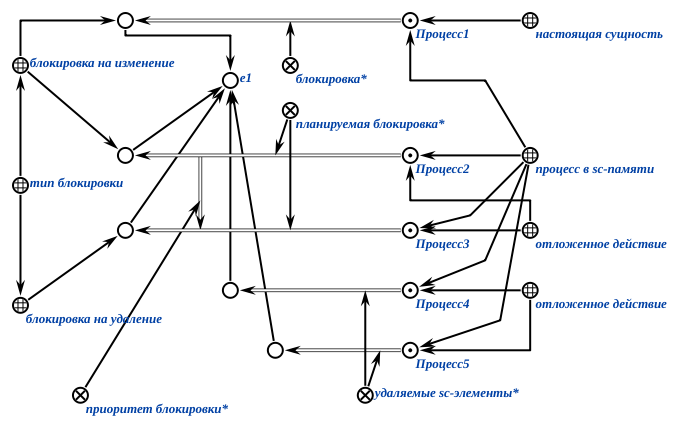
\includegraphics[scale=0.8]{images/part3/chapter_situation_management/plan_lock_1.png}
	\label{fig:plan_lock_1}
\end{figure}

В данном примере \textit{Процесс1} непосредственно работает с sc-элементом \textit{\textbf{e1}},\textit{Процесс2} и \textit{Процесс3} планируют установить блокировку на любое изменение и блокировку на удаление соответственно, причем \textit{Процесс2} попытался установить свою блокировку раньше, чем \textit{Процесс3}, поэтому согласно направлению связки отношения \textit{приоритет блокировки*}, его блокировка будет установлена раньше. \textit{Процесс4} и \textit{Процесс5} ожидают снятия всех блокировок и планируемых блокировок, после чего \textit{\textbf{e1}} будет удален и \textit{Процесс1} и \textit{Процесс2} продолжат свое выполнение. Никакие другие планируемые блокировки установлены быть уже не могут, поскольку \textit{\textbf{e1}} попал во множество удаляемых sc-элементов как минимум одного процесса и, в соответствии с изложеннымивыше правилами, все остальные процессы кроме \textit{Процесс1}-\textit{Процесс5}, уже несмогут получить доступ к этому sc-элементу.		
Выполняемый процесс принадлежит множеству настоящая сущность, приостановленные -- множеству отложенное действие.

\begin{figure}[H]
	\caption{SCg-текст. Пример использования планируемых блокировок (продолжение)}
	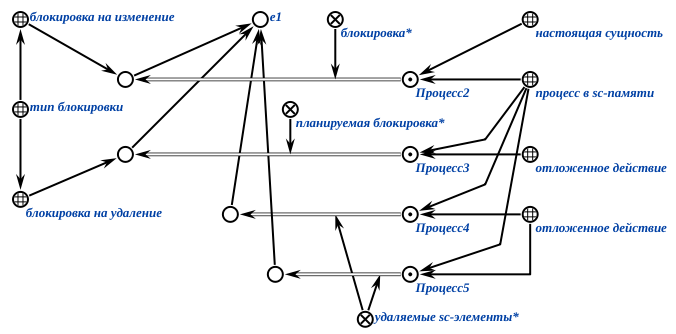
\includegraphics[scale=0.8]{images/part3/chapter_situation_management/plan_lock_2.png}
	\label{fig:plan_lock_2}
\end{figure}

После того как \textit{Процесс1} разблокировал sc-элемент \textit{\textbf{e1}}, этот элемент будет заблокирован \textit{Процессом2}, и \textit{Процесс2} продолжит выполнение. \textit{Планируемая блокировка*}, установленная \textit{Процессом2}, становится обычной \textit{блокировкой*}.

\begin{figure}[H]
	\caption{SCg-текст. Пример использования блокировки на удаление}
	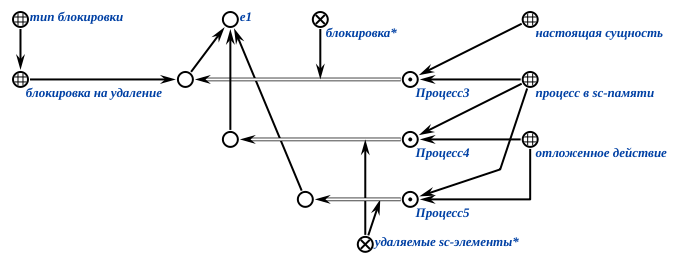
\includegraphics[scale=0.8]{images/part3/chapter_situation_management/plan_lock_3.png}
	\label{fig:plan_lock_3}
\end{figure}

После того как \textit{Процесс2} разблокировал sc-элемент \textit{\textbf{e1}}, этот элемент будет заблокирован \textit{Процессом3}, и \textit{Процесс3} продолжит выполнение.

\begin{figure}[H]
	\caption{SCg-текст. Удаляемые sc-элементы}
	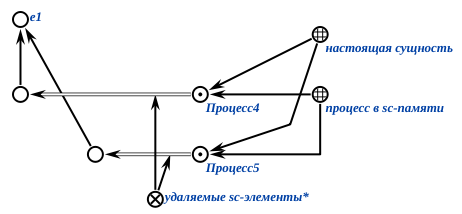
\includegraphics[scale=0.8]{images/part3/chapter_situation_management/plan_lock_4.png}
	\label{fig:plan_lock_4}
\end{figure}

Когда все процессы снимут блокировки с sc-элемента \textit{\textbf{e1}}, он может быть физически удален и \textit{Процесс4} и \textit{Процесс5} продолжат выполнение.

В зависимости от конкретных \textit{типов блокировок} установленных паралельно выполняемыми процессами на некоторые sc-элементы и того, какие конкретно действия с этими \textit{sc-элементами} предполагается выполнить далее в рамках выполнения этих процессов, возможны ситуации взаимоблокировки, когда каждый из указанных процессов будет ожидать снятия блокировки вторым процессом с нужного \textit{sc-элемента}, не снимая при этом установленной им самим блокировки с \textit{sc-элемента}, доступ к которому необходим второму процессу.
	
В случае когда хотя бы одна из блокировок является \textit{полной блокировкой}, ситуация взаимоблокировки возникнуть не может, поскольку \textit{sc-элементы}, попавшие в \textit{полную блокировку} некоторого \textit{scp-процесса}, не доступны другим \textit{scp-процессам} даже для чтения и, таким образом, остальные \textit{scp-процессы} будут работать так, как будто заблокированные \textit{sc-элементы} просто отсутствуют в текущем состоянии \textit{sc-памяти}.

В случаях, когда ни одна из установленных блокировок не является \textit{полной блокировкой}, возможно появление взаимоблокировок.

Устранение \textit{взаимоблокировки} невозможно без вмешательства специализированного \textit{sc-метаагента}, который имеет право игнорировать блокировки, установленные другими процессами. 
	
В общем случае проблема конкретной взаимоблокировки может быть решена путем выполнения специализированным \textit{sc-метаагентом} следующих шагов:	
\begin{textitemize}
	\item откат нескольких операций, выполненных одним из участвующих в взаимоблокировке процессов настолько шагов назад, насколько это необходимо для того, чтобы второй процесс получил доступ к необходимым \textit{sc-элементам} и смог продолжить выполнение;
	\item ожидание выполнения второго процесса вплоть до завершения или до снятия им всех блокировок с \textit{sc-элементов}, доступ к которым необходимо получить первому процессу;
	\item повторное выполнение в рамках первого процесса отмененных операций и продолжение его выполнения, но уже с учетом изменений в памяти, внесенных вторым процессом.		
\end{textitemize}

Для \textit{sc-метаагентов} все sc-элементы, в том числе описывающие блокировки, планируемые блокировки и так далее полностью эквивалентны между собой с точки зрения доступа к ним, то есть любой \textit{sc-метаагент} имеет доступ к любым sc-элементам, даже попавшим в полную блокировку для какого-либо другого процесса. Это необходимо для того, чтобы \textit{sc-метаагенты} смогли выявлять и устранять различные проблемы, например, описанную выше проблему взаимоблокировки.

Таким образом, проблема синхронизации деятельности \textit{sc-метаагентов} требует введения дополнительных правил.

Указанную проблему разделим на две более частные:
\begin{textitemize}
	\item обеспечение синхронизации деятельности \textit{sc-метаагентов} между собой;
	\item обеспечение синхронизации деятельности \textit{sc-метаагентов} и \textit{программных sc-агентов}.		
\end{textitemize}

Первую проблему предлагается решить за счет запрета параллельного выполнения \textit{sc-метаагентов}. Таким образом, в каждый момент времени в рамках одной \textit{ostis-системы} может существовать только один процесс, соответствующий \textit{sc-метаагенту} и являющийся \textit{настоящей сущностью}. 

Вторую проблему предлагается решить за счет введения дополнительных привилегий для \textit{sc-метаагентов} при обращении к какому-либо sc-элементу. Для этого достаточно одного правила: 

Если некоторый sc-элемент стал использоваться в рамках процесса, соответствующего \textit{sc-метаагенту} (например, стал элементом хотя бы одного scp-оператора, входящего в данный процесс), то все процессы, в блокировки соответствующие которым попадает указанный sc-элемент, становятся отложенными действиями (приостанавливают выполнение). Как только указанный sc-элемент перестает использоваться в рамках процесса, соответствующего \textit{sc-метаагенту}, все приостановленные по этой причине процессы продолжают выполнение.

Рассмотренные ограничения не ухудшают производительность \textit{ostis-системы} существенно, поскольку \textit{sc-мета\-аген\-ты} предназначены для решения достаточно узкого класса задач, которые, как показал опыт практической разработки прототипов различных \textit{ostis-систем}, возникают достаточно редко.
	
Стоит отметить, что возможна ситуация, при которой выполнение некоторого процесса в sc-памяти прервано по причине возникновения какой-либо ошибки. В таком случае существует вероятность того, что блокировка, установленная данным процессом не будет снята до тех пор, пока этого не сделает \textit{sc-метаагент}, обнаруживший подобную ситуацию. Однако указанная проблема на уровне sc-модели может быть решена лишь частично, для случаев, когда ошибка возникает при интерпретации \textit{scp-программы}, отслеживается \textit{scp-интепретатором} и в памяти формируется соответствующая конструкция, сообщающая о проблеме \textit{sc-метаагенту}. Случаи, когда возникла ошибка на уровне \textit{scp-интерпретатора} или \textit{sc-памяти}, должны рассматриваться на уровне \textit{ostis-платформы}.

\section{Базовый язык программирования ostis-систем}
\label{sec_ps_scp}

\begin{SCn}
\begin{scnrelfromlist}{подраздел}
	\scnitem{\ref{subsec_scp_denot}~\nameref{subsec_scp_denot}}
	\scnitem{\ref{subsec_scp_oper}~\nameref{subsec_scp_oper}}
\end{scnrelfromlist}

\bigskip

\begin{scnrelfromlist}{ключевой знак}
	\scnitem{Язык SCP}
	\scnitem{Абстрактная scp-машина}
\end{scnrelfromlist}
\begin{scnrelfromlist}{ключевое понятие}
	\scnitem{scp-оператор}
	\scnitem{параметр scp-программы\scnrolesign}
\end{scnrelfromlist}
\end{SCn}

Как было показано в \textit{\ref{sec_ps_agents} \nameref{sec_ps_agents}}, выделение Базового языка программирования для ostis-систем позволяет обеспечить четкое разделение уровня методов и соответственно, навыков ostis-системы, которые могут быть полностью описаны на уровне базы знаний и более низкоуровневых навыков, обеспечивающих интерпретацию указанных навыков более высокого уровня. Другими словами, выделение такого языка позволяет обеспечить \uline{платформенную независимость} ostis-систем, как в случае программной реализации \textit{ostis-платформы}, так и в случае \textit{ассоциативного семантического компьютера}.

В качестве базового языка для описания программ обработки текстов \textit{SC-кода} предлагается \textit{Язык SCP}. \textbf{\textit{Язык SCP}} -- это графовый язык процедурного программирования, предназначенный для эффективной обработки \textit{sc-текстов}. \textit{Язык SCP} является языком параллельного асинхронного программирования.

\bigskip
\bigskip

\begin{SCn}
	\scnheader{Язык SCP}
	\scnidtftext{часто используемый sc-идентификатор}{\textbf{\textit{scp-программа}}}
\end{SCn}

Языком представления данных для текстов \textit{Языка SCP} (\textit{scp-программ}) является \textit{SC-код} и, соответственно, любые варианты его внешнего представления. \textit{Язык SCP} сам построен на основе \textit{SC-кода}, вследствие чего \textit{scp-программы} сами по себе могут входить в состав обрабатываемых данных для \textit{scp-программ}, в том числе по отношению к самим себе. Таким образом, \textit{Язык SCP} предоставляет возможность построения реконфигурируемых программ. Однако для обеспечения возможности реконфигурирования программы непосредственно в процессе ее интерпретации необходимо на уровне интерпретатора \textit{Языка SCP (Aбстрактной scp-машины)} обеспечить уникальность каждой исполняемой копии исходной \textit{программы}. Такую исполняемую копию, сгенерированную на основе \textit{scp-программы}, будем называть \textit{scp-процессом}.
Включение знака некоторого \textit{действия в sc-памяти} во множество \textit{scp-процессов} гарантирует тот факт, что в декомпозиции данного действия будут присутствовать только знаки элементарных действий (\textit{scp-операторов}), которые может интерпретировать реализация \textit{Aбстрактной scp-машины} (интерпретатора scp-программ).

\textit{Язык SCP} рассматривается как ассемблер для \textit{ассоциативного семантического компьютера}.

\begin{SCn}
	\scnheader{Абстрактная scp-машина}
	\scniselement{scp-машина}
	\begin{scnindent}
		\scnrelto{обобщенная модель}{scp-интерпретатор}
	\end{scnindent}
\end{SCn}

\textit{Базовая модель обработки sc-текстов} включает в себя \textit{Предметную область Базового языка программирования ostis-систем}, то есть описание \textit{Синтаксиса} и \textit{Денотационной семантики Языка SCP}, а также описание \textit{Абстрактной scp-машины}, которая является моделью \textit{scp-интерпретатора}, который должен являться частью \textit{ostis-платформы} (хотя в общем случае могут существовать варианты платформы, не содержащие такого интерпретатора, что, однако, не позволит использовать достоинства предлагаемой базовой модели.

Рассмотрим ключевые особенности и достоинства \textit{Базовой модели обработки sc-текстов}:
\begin{textitemize}
	\item Тексты программ \textit{Языка SCP} записываются при помощи тех же унифицированных семантических сетей, что и обрабатываемая информация, таким образом, можно сказать, что \textit{Синтаксис Языка SCP} на базовом уровне совпадает с \textit{Синтаксисом SC-кода}.\item Подход к интерпретации \textit{scp-программ} предполагает создание при каждом вызове \textit{scp-программы} уникального \textit{scp-процесса}.
	\item Одновременно в общей памяти могут выполняться несколько независимых \textit{sc-агентов}, при этом разные копии \textit{sc-агентов} могут выполняться на разных серверах, за счет распределенной реализации \textit{ostis-платформы}. Более того, \textit{Язык SCP} позволяет осуществлять параллельные асинхронные вызовы подпрограмм с последующей синхронизацией, и даже параллельно	выполнять операторы в рамках одной \textit{scp-программы}.
	\item Перенос \textit{sc-агента} из одной системы в другую заключается в простом переносе фрагмента \textit{базы знаний}, без каких-либо дополнительных операций, зависящих от \textit{ostis-платформы}.
	\item Тот факт, что спецификации \textit{sc-агентов} и их программы могут быть записаны на том же языке, что и обрабатываемые знания, существенно сокращает перечень специализированных средств, предназначенных для проектирования машин обработки знаний, и упрощает их разработку за счет использования более универсальных компонентов.
	\item Тот факт, что для интерпретации \textit{scp-программы} создается соответствующий ей уникальный \textit{\mbox{scp-процесс}}, позволяет по возможности оптимизировать план выполнения перед его реализацией и даже непосредственно в процессе выполнения без потенциальной опасности испортить общий универсальный алгоритм всей программы. Более того, такой подход к проектированию и интерпретации программ позволяет говорить о возможности создания самореконфигурируемых программ.
\end{textitemize}

\begin{SCn}
\scnheader{scp-программа}
\scnsubset{программа в sc-памяти}
\scnsuperset{агентная scp-программа}
\end{SCn}

Каждая \textbf{\textit{scp-программа}} представляет собой обобщенную \textit{sc-структуру}, описывающую один из вариантов декомпозиции действий некоторого класса, выполняемых в sc-памяти. Знак \textit{sc-переменной}, соответствующей конкретному декомпозируемому действию является в рамках \textbf{\textit{scp-программы}} \textit{ключевым sc-элементом\scnrolesign}. Также явно указывается принадлежность данного знака множеству \textit{scp-процессов}.
	
Принадлежность некоторого действия множеству \textit{scp-процессов} гарантирует тот факт, что в декомпозиции данного действия будут присутствовать только знаки элементарных действий (\textit{scp-операторов}), которые может интерпретировать реализация \textit{Абстрактной scp-машины}.

Таким образом, каждая \textbf{\textit{scp-программа}} описывает в обобщенном виде декомпозицию некоторого \textit{\mbox{scp-процесса}} на взаимосвязанные \textit{scp-операторы}, с указанием, при их наличии, аргументов для данного \textit{scp-процесса}.

По сути каждая \textbf{\textit{scp-программа}} представляет собой описание последовательности элементарных операций, которые необходимо выполнить над семантической сетью, чтобы выполнить более сложное действие некоторого класса.

На рисунке \textit{\nameref{fig:program_example}} приведен пример простой \textit{scp-программы}. В приведенном примере показана \textit{scp-программа}, состоящая из трех \textit{scp-операторов}. Данная программа проверяет, содержится ли в заданном множестве (первый параметр) заданный элемент (второй параметр), и, если нет, то добавляет его в это множество.
	
\begin{figure}[H]
	\caption{SCg-текст. Пример scp-программы}
	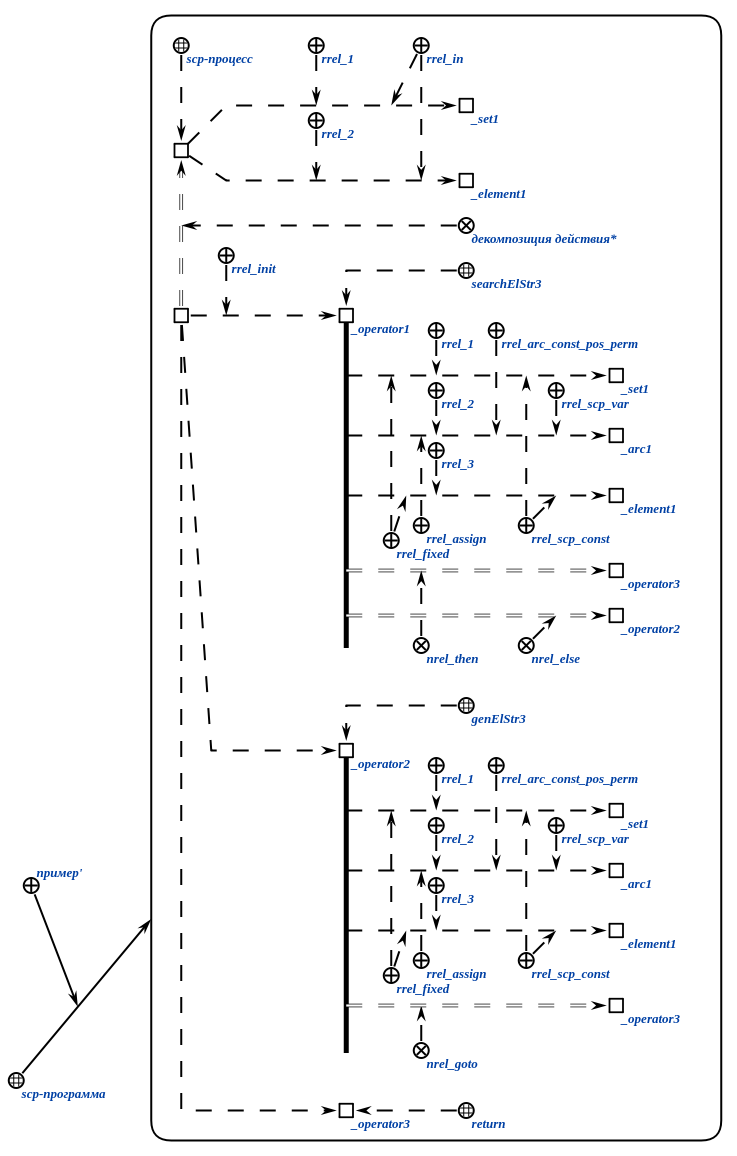
\includegraphics[scale=0.8]{images/part3/chapter_situation_management/program_example.png}
	\label{fig:program_example}
\end{figure}

\textbf{\textit{агентные scp-программы}} представляют собой частный случай \textit{scp-программ} вообще, однако заслуживают отдельного рассмотрения, поскольку используются наиболее часто. \textit{scp-программы} данного класса представляют собой реализации программ агентов обработки знаний, и имеют жестко фиксированный набор параметров. Каждая такая программа имеет ровно два \textit{in-параметра\scnrolesign}. Значение первого параметра является знаком бинарной ориентированной пары, являющейся вторым компонентом связки отношения \textit{первичное условие инициирования*} для абстрактного \textit{sc-агента}, в множество \textit{программ sc-агента*} которого входит рассматриваемая \textbf{\textit{агентная scp-программа}}, и, по сути, описывает класс событий, на которые реагирует указанный sc-агент.
	
Значением второго параметра является \textit{sc-элемент}, с которым непосредственно связано событие, в результате возникновения которого был инициирован соответствующий \textit{sc-агент}, то есть, например, сгенерированная либо удаляемая \textit{sc-дуга} или \textit{sc-ребро}.

Рассмотрим принципы реализации \textit{абстрактных sc-агентов, реализуемых на Языке SCP}:
\begin{textitemize}
\item общие принципы организации взаимодействия \textit{sc-агентов} и пользователей \textit{ostis-системы} через общую \textit{sc-память};
\item в результате появления в sc-памяти некоторой конструкции,
удовлетворяющей условию инициирования какого-либо \textit{абстрактного sc-агента}, реализованного при помощи \textit{Языка SCP}, в \textit{sc-памяти} генерируется и инициируется \textit{scp-процесс}. В качестве шаблона для генерации используется \textit{агентная scp-программа}, указанная во множестве программ соответствующего \textit{абстрактного sc-агента};
\item каждый такой \textit{scp-процесс}, соответствующий некоторой \textit{агентной scp-программе}, может быть связан с набором структур, описывающих блокировки различных типов. Таким образом, синхронизация взаимодействия параллельно выполняемых \textit{scp-процесcов} осуществляется так же, как и в случае любых других \textit{действий в sc-памяти};
\item В рамках \textit{scp-процесса} могут создаваться дочерние
\textit{scp-процессы}, однако синхронизация между ними при необходимости осуществляется посредством введения дополнительных внутренних блокировок. Таким образом, каждый \textit{scp-процесс} с точки зрения \textit{процессов в sc-памяти} является атомарным и законченным актом деятельности некоторого \textit{sc-агента};
\item во избежание нежелательных изменений в самом теле \textit{scp-процесса}, вся конструкция, сгенерированная на основе некоторой \textit{scp-программы} (весь текст \textit{scp-процесса}), должна быть добавлена в \textit{полную блокировку}, соответствующую данному \textit{scp-процессу};
\item все конструкции, сгенерированные в процессе выполнения
\textit{scp-процесса}, автоматически попадают в \textit{полную 	блокировку}, соответствующую данному \textit{scp-процессу}. Дополнительно следует отметить, что знак самой этой структуры и вся метаинформация о ней также включаются в эту структуру;
\item при необходимости можно вручную разблокировать или заблокировать некоторую конструкцию каким-либо типом блокировки, используя соответствующие \textit{scp-операторы} класса \textit{scp-оператор управления блокировками};
\item после завершения выполнения некоторого \textit{scp-процесса} его текст как правило, удаляется из \textit{\mbox{sc-памяти}}, а все заблокированные конструкции освобождаются (разрушаются знаки структур, обозначавших блокировки);
\item несмотря на то, что каждый \textit{scp-оператор} представляет собой атомарное \textit{действие в sc-памяти}, дополнительные блокировки, соответствующие одному оператору не вводятся, чтобы избежать громоздкости и избытка дополнительных системных конструкций, создаваемых при выполнении некоторого \textit{scp-процесса}. Вместо этого используются блокировки, общие для всего \textit{scp-процесса}. Таким образом, агенты \textit{Абстрактной scp-машины} при интерпретации \textit{scp-операторов} работают только с учетом блокировок, общих для всего интерпретируемого \textit{scp-процесса};
\item как правило, частный \textit{класс действий}, соответствующий конкретной \textit{scp-программе} явно не вводится, а используется более общий класс \textit{scp-процесс}, за исключением тех случаев, когда введение специального \textit{класса действий} необходимо по каким-либо другим соображениям.
\end{textitemize}

Под \textbf{\textit{scp-процессом}} понимается некоторое \textit{действие в sc-памяти}, однозначно описывающее конкретный акт выполнения некоторой \textit{scp-программы} для заданных исходных данных. Если \textit{scp-программа} описывает алгоритм решения какой-либо задачи в общем виде, то \textit{scp-процесс} обозначает конкретное действие, реализующее данный алгоритм для заданных входных параметров.

По сути, \textbf{\textit{scp-процесс}} представляет собой уникальную копию, созданную на основе \textit{scp-программы}, в которой каждой \textit{sc-переменной}, за исключением \textit{scp-переменных\scnrolesign}, соответствует сгенерированная \textit{sc-константа}.

Принадлежность некоторого действия множеству \textit{scp-процессов} гарантирует тот факт, что в декомпозиции данного действия будут присутствовать только знаки элементарных действий (\textit{scp-операторов}), которые может интерпретировать реализация \textit{Абстрактной scp-машины}.

Рассмотрим пример поэтапного выполнения scp-процесса (\textit{\nameref{fig:process_example}} -- \textit{\nameref{fig:process_example4}}), соответствующего ранее рассмотренному примеру scp-программы. В приведенном примере последовательно показаны состояния \textit{scp-процесса}, соответствующего \textit{\mbox{scp-программе}}, добавляющей заданный элемент в заданное множество, если он там ранее не содержался. В примере предполагается, что рассматриваемый элемент (\textit{Element1}) изначально не содержится во множестве (\textit{Set1}).

\begin{figure}[H]
	\caption{SCg-текст. Пример scp-процесса на начальной стадии выполнения}
	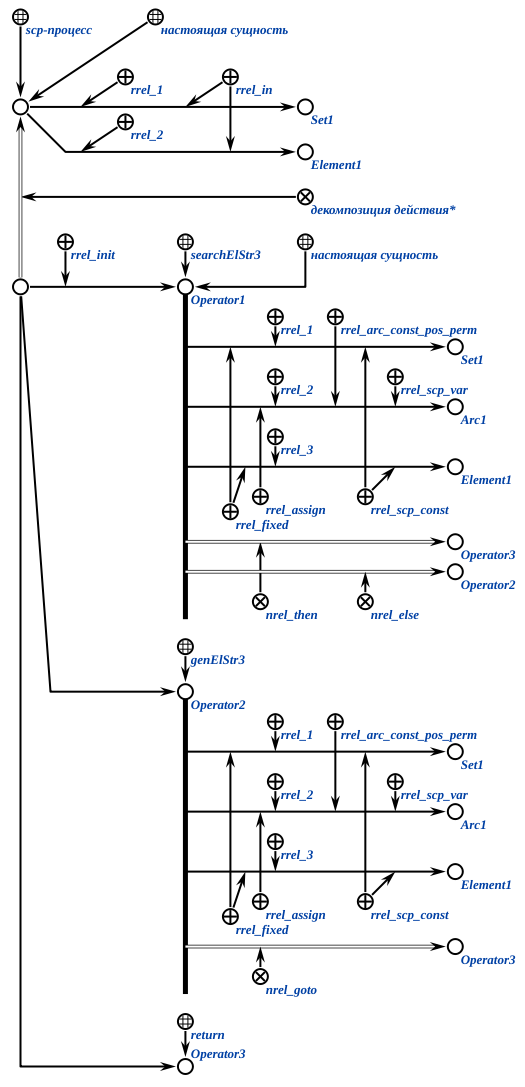
\includegraphics[scale=0.8]{images/part3/chapter_situation_management/process_example.png}
	\label{fig:process_example}
\end{figure}

Осуществляется вызов \textit{scp-программы}. Генерируется соответствующий \textit{scp-процесс}. Происходит инициирование начального оператора scp-процесса \textit{Operator1}.

\begin{figure}[H]
	\caption{SCg-текст. Пример scp-процесса: безуспешно выполнен оператор поиска}
	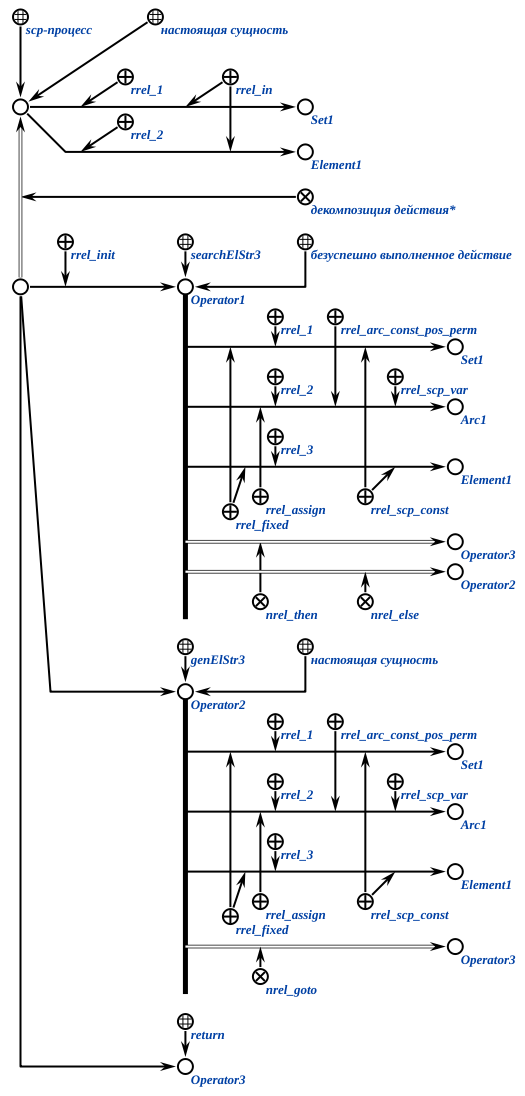
\includegraphics[scale=0.8]{images/part3/chapter_situation_management/process_example2.png}
	\label{fig:process_example2}
\end{figure}

Оператор \textit{Operator1} оказался безуспешно выполненным. Производится инициирование \textit{\mbox{scp-оператора} генерации трехэлементной конструкции} ~~~ \textit{Operator2}.

\begin{figure}[H]
	\caption{SCg-текст. Пример scp-процесса: выполнен оператор генерации, элемент добавлен во множество}
	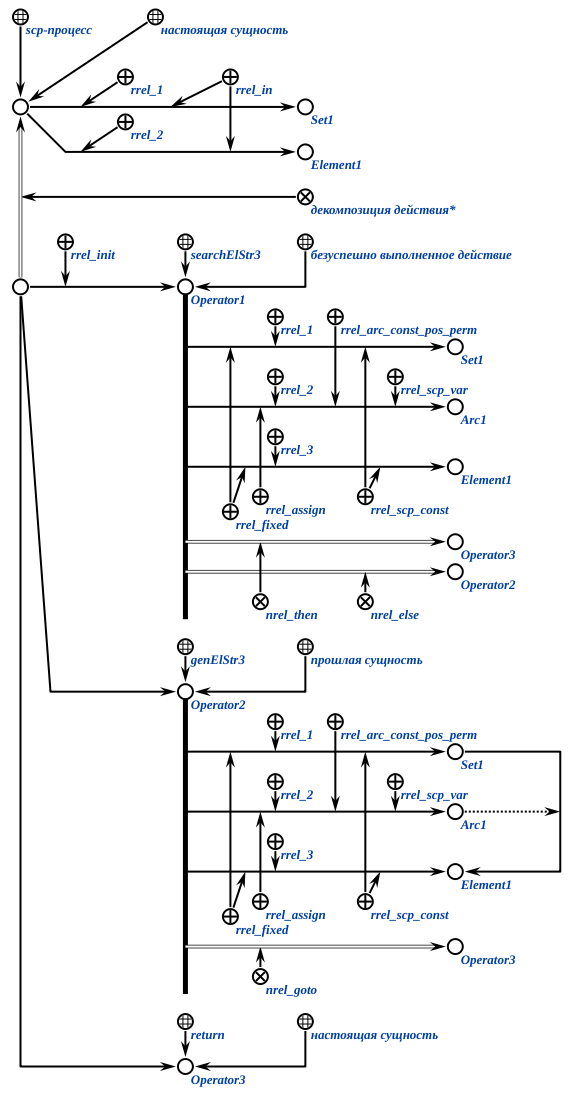
\includegraphics[scale=0.8]{images/part3/chapter_situation_management/process_example3.png}
	\label{fig:process_example3}
\end{figure}

Оператор \textit{Operator2} выполнился. Производится инициирование \textit{scp-оператора завершения выполнения программы} ~~~ \textit{Operator3}.

\begin{figure}[H]
	\caption{SCg-текст. Пример scp-процесса: выполнение завершено}
	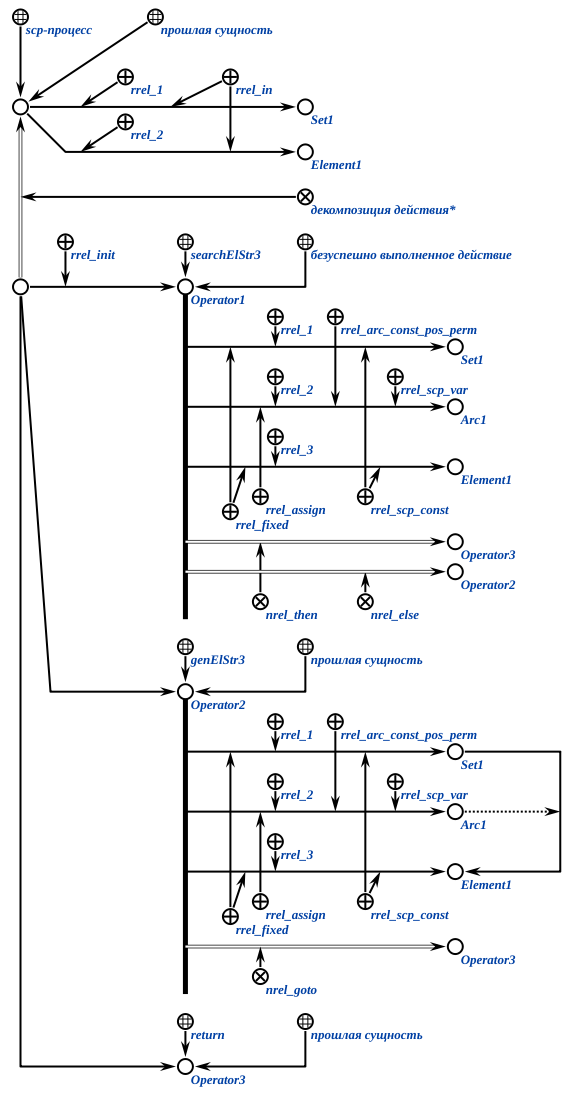
\includegraphics[scale=0.8]{images/part3/chapter_situation_management/process_example4.png}
	\label{fig:process_example4}
\end{figure}

Оператор \textit{Operator3} выполнился. Выполнение \textit{scp-процесса} завершается.

\begin{SCn}
\scnheader{scp-оператор}
\scnsubset{действие в sc-памяти}
\scnrelto{семейство подмножеств}{атомарный тип scp-оператора}
\end{SCn}

Каждый \textbf{\textit{scp-оператор}} представляет собой некоторое элементарное \textit{действие в sc-памяти}. Аргументы \textit{scp-оператора} будем называть операндами. Порядок операндов указывается при помощи соответствующих ролевых отношений (\textit{1\scnrolesign}, \textit{2\scnrolesign}, \textit{3\scnrolesign} и так далее). Операнд, помеченный ролевым отношением \textit{1\scnrolesign}, будем называть первым операндом, помеченный ролевым отношением \textit{2\scnrolesign} --- вторым операндом, и т.д. Тип и смысл каждого операнда также уточняется при помощи различных подклассов отношения \textit{scp-операнд\scnrolesign}. В общем случае операндом может быть любой \textit{sc-элемент}, в том числе, знак какой-либо \textit{scp-программы}, в том числе самой программы, содержащей данный оператор.

Каждый \textbf{\textit{scp-оператор}} должен иметь один и более операнд, а также указание того \textbf{\textit{scp-оператора}} (или нескольких), который должен быть выполнен следующим. Исключение их данного правила составляет \textit{scp-оператор завершения выполнения программы}, который не содержит ни одного операнда и после выполнения которого никакие \textit{scp-операторы} в рамках данной программы выполняться не могут.

Каждый \textbf{\textit{атомарный тип scp-оператора}} представляет собой класс \textit{scp-операторов}, который не разбивается на более частные, и, соответственно, интерпретируется реализацией \textit{Aбстрактной scp-машины}.

\begin{SCn}
\scnheader{начальный оператор\scnrolesign}
\scnsubset{1\scnrolesign}
\end{SCn}

Ролевое отношение \textbf{\textit{начальный оператор\scnrolesign}} указывает в рамках декомпозиции соответствующего \textit{\mbox{scp-программе}} \textit{scp-процесса} те \textit{scp-операторы}, которые должны быть выполнены в первую очередь, то есть те, с которых собственно начинается выполнение \textit{scp-процесса}.

\begin{SCn}
\scnheader{параметр scp-программы\scnrolesign}
\scnsubset{аргумент действия\scnrolesign}
\begin{scnrelfromset}{разбиение}
	\scnitem{in-параметр\scnrolesign}
	\scnitem{out-параметр\scnrolesign}
\end{scnrelfromset}
\end{SCn}

Ролевое отношение \textbf{\textit{параметр scp-программы\scnrolesign}} связывает знак соответствующего \textit{scp-программе} \textit{\mbox{scp-процесса}} с его аргументами.

Параметры типа \textbf{\textit{in-параметр\scnrolesign}} хоть и соответствуют \textit{переменным scp-программы\scnrolesign}, не могут менять значение в процессе ее интерпретации. Фиксированное значение переменной устанавливается при создании уникальной копии \textit{scp-программы} (\textit{scp-процесса}) для ее интерпретации, и, таким образом, соответствующая \textit{scp-переменная\scnrolesign} на момент начала ее интерпретации становится \textit{scp-константой\scnrolesign} в рамках каждого \textit{scp-оператора}, в котором встречалась данная \textit{scp-переменная\scnrolesign}. Использование \textit{in-параметров} можно рассматривать по аналогии с использованием варианта механизма передачи по значению в традиционных языках программирования, с тем условием, что значение локальной переменной в рамках дочерней программы не может быть изменено.

Параметры типа \textbf{\textit{out-параметр\scnrolesign}} соответствуют \textit{переменным scp-программы\scnrolesign} и обладают всеми теми же соответствующими свойствами. Чаще всего предполагается, что значение данного параметра необходимо родительской \textit{scp-программе}, содержащей оператор вызова текущей \textit{scp-программы}. При этом на момент начала интерпретации в качестве параметра дочернему процессу передается непосредственно узел, обозначающий переменную (а точнее, ее уникальную копию в рамках процесса) родительского процесса. Указанная переменная может при необходимости иметь значение, либо не иметь. После завершения и во время интерпретации дочернего процесса родительский процесс по-прежнему может работать с переменной, переданной в качестве \textit{out-параметра\scnrolesign}, при необходимости просматривая или изменяя ее значение. Использование out-параметра можно рассматривать по аналогии с использованием механизма передачи по ссылке в традиционных \textit{языках программирования}.

Рассмотрим классификацию \textit{sc-конструкций} с точки зрения \textit{Базовой модели обработки sc-текстов}.

\begin{SCn}
\scnheader{sc-конструкция}
\scnrelfrom{разбиение}{Классификация sc-конструкций с точки зрения Базовой модели обработки sc-текстов}
\begin{scnindent}
	\begin{scneqtoset}
		\scnitem{sc-конструкция нестандартного вида}
		\scnitem{sc-конструкция стандартного вида}
	\end{scneqtoset}
\begin{scnindent}
\begin{scnrelfromset}{разбиение}
	\scnitem{одноэлементная sc-конструкция}
	\scnitem{трехэлементная sc-конструкция}
	\scnitem{пятиэлементная sc-конструкция}	
\end{scnrelfromset}
\end{scnindent}
\end{scnindent}
\end{SCn}

Каждая \textit{sc-конструкция нестандартного вида} состоит из произвольного количества \textit{sc-элементов} произвольного типа (\textit{\nameref{fig:pic_ps4}}).

\begin{figure}[H]
	\caption{SCg-текст. Пример sc-конструкции нестандартного вида}
	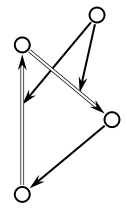
\includegraphics[scale=0.8]{images/part3/chapter_situation_management/pic_ps1.png}
	\label{fig:pic_ps1}
\end{figure}

В свою очередь, каждый элемент \textit{\mbox{sc-конструкции} стандартного вида} имеет свою условную строго фиксированную позицию в рамках этой \mbox{sc-конструкции} (первый элемент, второй элемент и так далее). В зависимости от указанной позиции вводятся дополнительные ограничения на тип соответствующего \textit{sc-элемента}.

Каждая \textit{одноэлементная sc-конструкция} состоит из одного \textit{sc-элемента} произвольного типа (Рис. \textit{\nameref{fig:pic_ps2}}).

\begin{figure}[H]
	\caption{SCg-текст. Пример одноэлементных sc-конструкций в SCg-коде}
	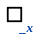
\includegraphics[scale=0.8]{images/part3/chapter_situation_management/pic_ps2.png}
	\label{fig:pic_ps2}
\end{figure}

Каждая \textit{трехэлементная sc-конструкция} состоит из трех \textit{sc-элементов} (Рис. \textit{\nameref{fig:pic_ps3}}). Второй элемент всегда является \textit{sc-коннектором}, остальные элементы могут быть произвольного типа.

\begin{figure}[H]
	\caption{SCg-текст. Пример трехэлементной sc-конструкции в SCg-коде}
	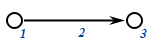
\includegraphics[scale=0.8]{images/part3/chapter_situation_management/pic_ps3.png}
	\label{fig:pic_ps3}
\end{figure}

Каждая \textit{пятиэлементная sc-конструкция} состоит из пяти \textit{sc-элементов} (Рис. \textit{\nameref{fig:pic_ps4}}). Второй и четвертый элементы обязательно являются \textit{sc-коннекторами}, остальные элементы могут быть произвольного типа.

\begin{figure}[H]
	\caption{SCg-текст. Пример пятиэлементной sc-конструкции в SCg-коде}
	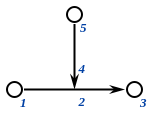
\includegraphics[scale=0.8]{images/part3/chapter_situation_management/pic_ps4.png}
	\label{fig:pic_ps4}
\end{figure}

\subsection{Денотационная семантика Базового языка программирования ostis-систем}
\label{subsec_scp_denot}

\begin{SCn}
\begin{scnrelfromlist}{ключевое понятие}
	\scnitem{scp-оператор}
	\scnitem{scp-операнд\scnrolesign}
\end{scnrelfromlist}
\end{SCn}

\begin{SCn}
\scnheader{scp-оператор}
\scnsubset{действие в sc-памяти}
\scnrelto{семейство подмножеств}{атомарный тип scp-оператора}
\begin{scnrelfromset}{разбиение}
	\scnitem{scp-оператор генерации конструкций}
	\begin{scnindent}
		\begin{scnrelfromset}{разбиение}
			\scnitem{scp-оператор генерации конструкции по произвольному образцу}
			\scnitem{scp-оператор генерации пятиэлементной конструкции}
			\scnitem{scp-оператор генерации трехэлементной конструкции}
			\scnitem{scp-оператор генерации одноэлементной конструкции}
		\end{scnrelfromset}
	\end{scnindent}
	\scnitem{scp-оператор ассоциативного поиска конструкций}
	\begin{scnindent}
		\begin{scnrelfromset}{разбиение}
			\scnitem{scp-оператор поиска конструкции по произвольному образцу}
			\scnitem{scp-оператор поиска пятиэлементной конструкции с формированием множеств}
			\scnitem{scp-оператор поиска трехэлементной конструкции с формированием множеств}
			\scnitem{scp-оператор поиска пятиэлементной конструкции}
			\scnitem{scp-оператор поиска трехэлементной конструкции}
		\end{scnrelfromset}
	\end{scnindent}
	\scnitem{scp-оператор удаления конструкций}
	\begin{scnindent}
		\begin{scnrelfromset}{разбиение}
			\scnitem{scp-оператор удаления множества элементов трехэлементной конструкции}
			\scnitem{scp-оператор удаления одноэлементной конструкции}
			\scnitem{scp-оператор удаления пятиэлементной конструкции}
			\scnitem{scp-оператор удаления трехэлементной конструкции}
		\end{scnrelfromset}
	\end{scnindent}
	\scnitem{scp-оператор проверки условий}
	\begin{scnindent}
		\begin{scnrelfromset}{разбиение}
			\scnitem{scp-оператор сравнения числовых содержимых файлов}
			\scnitem{scp-оператор проверки равенства числовых содержимых файлов}
			\scnitem{scp-оператор проверки совпадения значений операндов}
			\scnitem{scp-оператор проверки наличия содержимого у файла}
			\scnitem{scp-оператор проверки наличия значения у переменной}
			\scnitem{scp-оператор проверки типа sc-элемента}
		\end{scnrelfromset}
	\end{scnindent}
	\scnitem{scp-оператор управления значениями операндов}
	\begin{scnindent}
		\begin{scnrelfromset}{разбиение}
			\scnitem{scp-оператор удаления значения переменной}
			\scnitem{scp-оператор присваивания значения переменной}
		\end{scnrelfromset}
	\end{scnindent}
	\scnitem{scp-оператор управления scp-процессами}
	\begin{scnindent}
		\begin{scnrelfromset}{разбиение}
			\scnitem{scp-оператор удаления значения переменной}
			\scnitem{scp-оператор завершения выполнения программы}
			\scnitem{конъюнкция предшествующих scp-операторов}
			\scnitem{scp-оператор ожидания завершения выполнения множества scp-программ}
			\scnitem{scp-оператор ожидания завершения выполнения scp-программы}
			\scnitem{scp-оператор асинхронного вызова подпрограммы}
		\end{scnrelfromset}
	\end{scnindent}
	\scnitem{scp-оператор управления событиями}
	\begin{scnindent}
		\scnsuperset{scp-оператор ожидания события}
	\end{scnindent}
	\scnitem{scp-оператор обработки содержимых файлов}
	\begin{scnindent}
		\begin{scnrelfromset}{разбиение}
			\scnitem{scp-оператор вычисления арксинуса числового содержимого файла}
			\scnitem{scp-оператор вычисления арккосинуса числового содержимого файла}
			\scnitem{scp-оператор деления числовых содержимых файлов}
			\scnitem{scp-оператор умножения числовых содержимых файлов}
			\scnitem{scp-оператор вычитания числовых содержимых файлов}
			\scnitem{scp-оператор сложения числовых содержимых файлов}
			\scnitem{scp-оператор вычисления тангенса числового содержимого файла}
			\scnitem{scp-оператор вычисления косинуса числового содержимого файла}
			\scnitem{scp-оператор вычисления синуса числового содержимого файла}
			\scnitem{scp-оператор вычисления логарифма числового содержимого файла}
			\scnitem{scp-оператор возведения числового содержимого файла в степень}
			\scnitem{scp-оператор удаления содержимого файла}
			\scnitem{scp-оператор копирования содержимого файла}
			\scnitem{scp-оператор нахождения остатка от деления числовых содержимых файлов}
			\scnitem{scp-оператор нахождения целой части от деления числовых содержимых файлов}
			\scnitem{scp-оператор вычисления арктангенса числового содержимого файла}
			\scnitem{scp-оператор перевода в верхний регистр строкового содержимого файла}
			\scnitem{scp-оператор перевода в верхний регистр строкового содержимого файла}
			\scnitem{scp-оператор замены определенной части строкового содержимого файла на содержимое указанной файла}
			\scnitem{scp-оператор проверки совпадения конца строкового содержимого файла со строковом содержимым другого файла}
			\scnitem{scp-оператор проверки совпадения начальной части строкового содержимого файла со строковом содержимым другого файла}
			\scnitem{scp-оператор получения части строкового содержимого файла по индексам}
			\scnitem{scp-оператор поиска строкового содержимого файла в строковом содержимом другого файла}
			\scnitem{scp-оператор вычисления длины строкового содержимого файла}
			\scnitem{scp-оператор разбиения строки на подстроки}
			\scnitem{scp-оператор лексикографического сравнения строковых содержимых файлов}
			\scnitem{scp-оператор проверки равенства строковых содержимых файлов}
		\end{scnrelfromset}
	\end{scnindent}
	\scnitem{scp-оператор управления блокировками}
	\begin{scnindent}
		\begin{scnrelfromset}{разбиение}
			\scnitem{scp-оператор снятия всех блокировок данного scp-процесса}
			\scnitem{scp-оператор снятия блокировки с sc-элемента}
			\scnitem{scp-оператор установки полной блокировки на sc-элемент}
			\scnitem{scp-оператор установки блокировки на изменение sc-элемента}
			\scnitem{scp-оператор установки блокировки на удаление sc-элемента}
			\scnitem{scp-оператор снятия блокировки со структуры}
			\scnitem{scp-оператор установки полной блокировки на структуру}
			\scnitem{scp-оператор установки блокировки на изменение структуры}
			\scnitem{scp-оператор установки блокировки на удаление структуры}
		\end{scnrelfromset}
	\end{scnindent}
\end{scnrelfromset}

\scnheader{scp-операнд\scnrolesign}
\scnsubset{аргумент действия\scnrolesign}
\scniselement{неосновное понятие}
\scniselement{ролевое отношение}
\begin{scnrelfromset}{разбиение}
	\scnitem{scp-константа\scnrolesign}
	\scnitem{scp-переменная\scnrolesign}
\end{scnrelfromset}	
\begin{scnrelfromset}{разбиение}
	\scnitem{scp-операнд с заданным значением\scnrolesign}
	\scnitem{scp-операнд со свободным значением\scnrolesign}
\end{scnrelfromset}	
\begin{scnrelfromset}{разбиение}
	\scnitem{константный sc-элемент\scnrolesign}
	\scnitem{переменный sc-элемент\scnrolesign}
\end{scnrelfromset}	
\begin{scnrelfromlist}{включение}
	\scnitem{формируемое множество\scnrolesign}
	\begin{scnindent}
		\begin{scnrelfromset}{разбиение}
			\scnitem{формируемое множество 1\scnrolesign}
			\scnitem{формируемое множество 2\scnrolesign}
			\scnitem{формируемое множество 3\scnrolesign}
			\scnitem{формируемое множество 4\scnrolesign}
			\scnitem{формируемое множество 5\scnrolesign}
		\end{scnrelfromset}	
	\end{scnindent}
	\scnitem{удаляемый sc-элемент\scnrolesign}
	\scnitem{тип sc-элемента\scnrolesign}
	\begin{scnindent}
	\begin{scnrelfromset}{разбиение}
		\scnitem{sc-узел\scnrolesign}
		\begin{scnindent}
			\begin{scnrelfromset}{разбиение}
				\scnitem{структура\scnrolesign}
				\scnitem{отношение\scnrolesign}
				\begin{scnindent}
					\scnsuperset{ролевое отношение\scnrolesign}
				\end{scnindent}
			\scnitem{класс\scnrolesign}
			\end{scnrelfromset}	
		\end{scnindent}
		\scnitem{sc-дуга\scnrolesign}
		\begin{scnindent}
			\begin{scnrelfromset}{разбиение}
				\scnitem{sc-дуга общего вида\scnrolesign}
				\scnitem{sc-дуга принадлежности\scnrolesign}
				\begin{scnindent}
					\scnsuperset{sc-дуга основного вида\scnrolesign}
					\begin{scnindent}
					\scneq{(константный sc-элемент\scnrolesign $\cap$ позитивная sc-дуга принадлежности\scnrolesign $\cap$ постоянная sc-дуга принадлежности\scnrolesign)}
					\end{scnindent}					
					\begin{scnrelfromset}{разбиение}
						\scnitem{позитивная sc-дуга принадлежности\scnrolesign}
						\scnitem{негативная sc-дуга принадлежности\scnrolesign}
						\scnitem{нечеткая sc-дуга принадлежности\scnrolesign}
					\end{scnrelfromset}
					\begin{scnrelfromset}{разбиение}
						\scnitem{временная sc-дуга принадлежности\scnrolesign}
						\scnitem{постоянная sc-дуга принадлежности\scnrolesign}
					\end{scnrelfromset}
				\end{scnindent}
			\end{scnrelfromset}
		\end{scnindent}
		\scnitem{sc-ребро\scnrolesign}
		\scnitem{файл\scnrolesign}
	\end{scnrelfromset}
	\end{scnindent}
\end{scnrelfromlist}
\end{SCn}

Ролевое отношение \textit{scp-операнд\scnrolesign} является неосновным понятием и указывает на принадлежность аргументов \textit{scp-оператору}. Помимо указания какого-либо класса \textit{scp-операндов\scnrolesign} порядок аргументов \textit{scp-оператора} дополнительно уточняется \textit{ролевыми отношениями 1\scnrolesign}, \textit{2\scnrolesign} и так далее

В рамках \textit{scp-программы} \textbf{\textit{scp-константы\scnrolesign}} явно участвуют в \textit{\mbox{scp-операторах}} в качестве элементов (в теоретико-множественном смысле) и напрямую обрабатываются при интерпретации \textit{scp-программы}. Константами в рамках \textit{scp-программы} могут быть \textit{sc-элементы} любого типа, как \textit{\mbox{sc-константы}}, так и \textit{\mbox{sc-переменные}}. Константа в рамках \textit{scp-программы} остается неизменной в течение всего срока интерпретации. Константа \textit{\mbox{scp-программы}} может быть рассмотрена как переменная, значение которой совпадает с самой переменной в каждый момент времени, и изменено быть не может. Таким образом, далее будем считать, что \textit{scp-константа\scnrolesign} и ее значение это одно и то же. Каждый \textit{in-параметр\scnrolesign} при интерпретации каждой конкретной копии \textit{scp-программы} становится \textit{scp-константой\scnrolesign} в рамках всех ее операторов, хотя в исходном теле данной программы в каждом из этих операторов он является \textit{scp-переменной\scnrolesign}.

В рамках \textit{scp-программы} \textbf{\textit{scp-переменные\scnrolesign}} не обрабатываются явно при интерпретации, обрабатываются значения переменных. Каждая переменная \textit{scp-программы} может иметь одно значение в каждый момент времени, то есть представляет собой ситуативный \textit{синглетон}, элементом которого является текущее значение \textit{scp-переменной\scnrolesign}. Значение каждой \textit{scp-переменной\scnrolesign} может меняться в ходе интерпретации \textit{scp-программы}. При этом интерпретатор при обработке \textit{scp-оператора} работает непосредственно со значениями \textit{\mbox{scp-переменных\scnrolesign}}, а не самими \textit{scp-переменными\scnrolesign} (которые также являются узлами той же семантической сети).

Значение операндов, помеченных ролевым отношением \textbf{\textit{scp-операнд с заданным значением\scnrolesign}}, считается заданным в рамках текущего \textit{scp-оператора}. Данное значение учитывается при выполнении \textit{scp-оператора} и остается неизменным после окончания выполнения \textit{scp-оператора}. Каждая \textit{scp-константа\scnrolesign} по умолчанию рассматривается как \textit{scp-операнд с заданным значением\scnrolesign}, в связи с чем явное использование данного ролевого отношения в таком случае является избыточным. В таком случае в качестве значения рассматривается непосредственно сам операнд. В случае если отношением \textit{\mbox{scp-операнд} с заданным значением\scnrolesign} помечена \textit{scp-переменная\scnrolesign}, то осуществляется попытка поиска значения для данной \textit{scp-переменной\scnrolesign} (ее элемента). Если попытка оказалась безуспешной, то возникает ошибка времени выполнения, которая должна быть обработана соответствующим образом.
	
Любой \textit{scp-операнд с заданным значением\scnrolesign} независимо от конкретного типа \textit{scp-оператора} может быть \textit{scp-переменной\scnrolesign}.

Значение операндов, помеченных ролевым отношением \textit{scp-операнд со свободным значением\scnrolesign}, считается свободным (не заданным заранее) в рамках текущего \textit{scp-оператора}. В начале выполнения \textit{scp-оператора} связь между \textit{scp-переменной\scnrolesign}, помеченной данным ролевым отношением, и ее элементом (значением) всегда удаляется. В результате выполнения данного оператора может быть либо сгенерировано новое значение \textit{scp-переменной\scnrolesign}, либо не сгенерировано, тогда \textit{scp-переменная\scnrolesign} будет считаться не имеющей значения. Ни одна \textit{scp-константа\scnrolesign} не может быть помечена как \textit{scp-операнд со свободным значением\scnrolesign}, поскольку константа не может изменять свое значение в ходе интерпретации \textit{scp-программы}.

Ролевое отношение \textit{тип \mbox{sc-элемента\scnrolesign}} используется для уточнения типа \textit{sc-элемента}, выступающего в роли значения некоторого операнда. \textit{тип \mbox{sc-элемента\scnrolesign}} имеет смысл указывать только для операндов, помеченных как \textit{scp-операнд со свободным значением\scnrolesign}, тогда данное уточнение типа \textit{\mbox{sc-элемента}} будет использовано для сужения области поиска либо уточнения параметров генерации каких-либо конструкций. Значением \textit{scp-операндов с заданным значением\scnrolesign} является конкретный, известный на момент начала выполнения \textit{scp-оператора sc-элемент} с конкретным типом, не зависящим от указания \textit{типа sc-элемента\scnrolesign}, в связи с чем использование ролевого отношения \textit{тип sc-элемента\scnrolesign} в данном случае является некорректным.

Допускается использование комбинаций семантически непротиворечащих друг другу подмножеств указанного отношения. Например, допускается комбинация \textit{константный sc-элемент\scnrolesign} и \textit{sc-дуга общего вида\scnrolesign}, но не допускается комбинация \textit{sc-узел\scnrolesign} и \textit{sc-дуга\scnrolesign}.

Ролевое отношение \textbf{\textit{формируемое множество\scnrolesign}} используется для указания того факта, что в результате выполнения \textit{scp-оператора} должно быть сформировано либо дополнено некоторое множество \textit{sc-элементов}, являющееся значением одного из операндов данного \textit{scp-оператора}. При этом если данный операнд помечен как \textit{scp-операнд со свободным значением\scnrolesign}, то множество будет сформировано с нуля (сгенерирован новый \textit{sc-элемент}, обозначающий данное множество), в противном случае уже существующее множество может быть дополнено. Использование данного ролевого отношения предполагает, что при его отсутствии множество бы не формировалось, а значением указанного операнда стал бы произвольный \textit{sc-элемент} из данного множества. 

Ролевое отношение \textit{формируемое множество\scnrolesign} без уточнения порядкового номера используется только в \textit{scp-операторах обработки произвольных конструкций}. Для явного указания номера операнда, которому соответствует \textit{формируемое множество\scnrolesign}, используются подмножества данного ролевого отношения, аналогичные ролевым отношениям, задающим порядок элементов в кортеже (\textit{1\scnrolesign, 2\scnrolesign, 3\scnrolesign} и так далее), например \textit{формируемое множество 1\scnrolesign}, \textit{формируемое множество 2\scnrolesign} и так далее. Указанные ролевые отношения используются только в \textit{scp-операторах поиска конструкций с формированием множеств}.

Ролевое отношение \textbf{\textit{удаляемый sc-элемент\scnrolesign}} используется для указания тех операндов, значение которых должно быть удалено в процессе выполнения \textit{scp-операторов удаления}. Данным ролевым отношением может быть помечен как \textit{scp-операнд с заданным значением\scnrolesign}, так и \textit{scp-операнд со свободным значением\scnrolesign}. При этом удаляемым \textit{sc-элементом} может быть как \textit{scp-константа\scnrolesign}, так и \textit{scp-переменная\scnrolesign} (в случае \textit{scp-переменной\scnrolesign} удаляется не только связка принадлежности между этой \textit{scp-переменной\scnrolesign} и ее значением, но и непосредственно сам \textit{sc-элемент}, являющийся значением).

\begin{SCn}
\scnheader{следует отличать*}
\begin{scnhaselementset}
	\scnitem{scp-переменная\scnrolesign}
	\scnitem{sc-переменная}	
\end{scnhaselementset}
\begin{scnhaselementset}
	\scnitem{scp-константа\scnrolesign}
	\scnitem{sc-константа}	
\end{scnhaselementset}
\end{SCn}

На рисунках \textit{\nameref{fig:genElStr5_fafaa}} -- \textit{\nameref{fig:genElStr5_fafaa_2}} показан пример работы scp-оператора генерации пятиэлементной конструкции. В приведенном примере выполняется генерация пятиэлементной конструкции, которая имеет два scp-операнда с заданным значением. В примере предполагается, что рассматриваемые элементы (some\_node1 и some\_node2) изначально никак не связаны между собой.

\begin{figure}[H]
	\caption{SCg-текст. Пример выполнения scp-оператора генерации пятиэлементной конструкции (вызов scp-оператора)}
	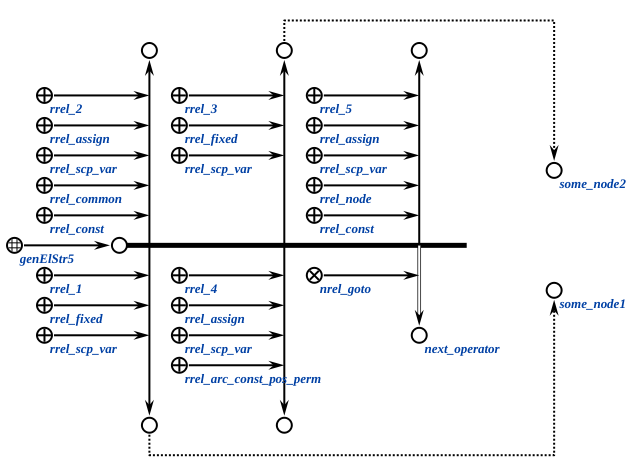
\includegraphics[scale=0.8]{images/part3/chapter_situation_management/genElStr5_fafaa.png}
	\label{fig:genElStr5_fafaa}
\end{figure}

\begin{figure}[H]
	\caption{SCg-текст. Пример выполнения scp-оператора генерации пятиэлементной конструкции (результат выполнения scp-оператора)}
	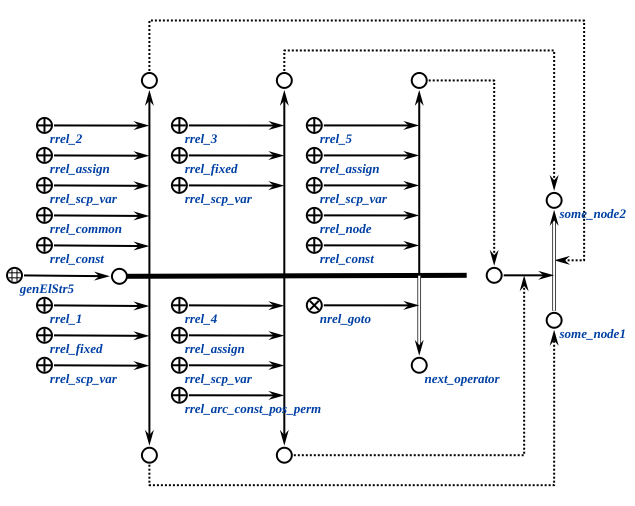
\includegraphics[scale=0.8]{images/part3/chapter_situation_management/genElStr5_fafaa_2.png}
	\label{fig:genElStr5_fafaa_2}
\end{figure}

На рисунках \textit{\nameref{fig:searchElStr3_faf}} -- \textit{\nameref{fig:searchElStr3_faf_2}} приведен пример scp-оператора поиска трехэлементной конструкции, которая имеет два scp-операнда с заданным значением. В примере предполагается, что рассматриваемые элементы (some\_node1 и some\_node2) изначально связаны между собой константной постоянной sc-дугой.

\begin{figure}[H]
	\caption{SCg-текст. Пример выполнения scp-оператора поиска трехэлементной конструкции (вызов scp-оператора)}
	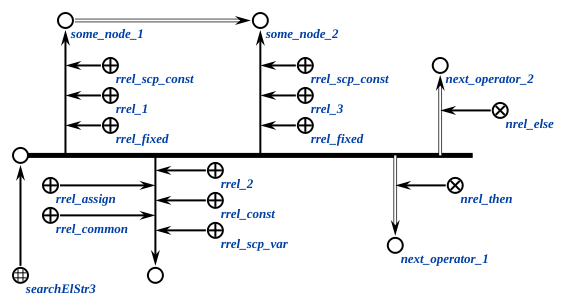
\includegraphics[scale=0.8]{images/part3/chapter_situation_management/searchElStr3_faf.png}
	\label{fig:searchElStr3_faf}
\end{figure}

\begin{figure}[H]
	\caption{SCg-текст. Пример выполнения scp-оператора поиска трехэлементной конструкции (результат выполнения scp-оператора)}
	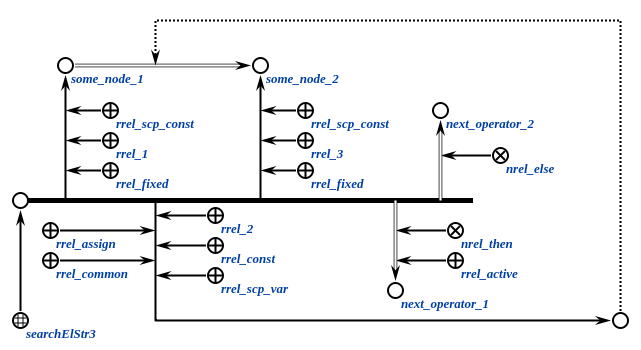
\includegraphics[scale=0.8]{images/part3/chapter_situation_management/searchElStr3_faf_2.png}
	\label{fig:searchElStr3_faf_2}
\end{figure}

На рисунках \textit{\nameref{fig:erase_edge}} -- \textit{\nameref{fig:erase_edge_2}} показан пример scp-оператора удаления одноэлементной конструкции. В примере предполагается, что рассматриваемые элементы (\textbf{\textit{node1}} и \textbf{\textit{node2}}) изначально связаны между собой базовой sc-дугой принадлежности.

\begin{figure}[H]
	\caption{SCg-текст. Пример выполнения scp-оператора удаления одноэлементной конструкции (вызов scp-оператора)}
	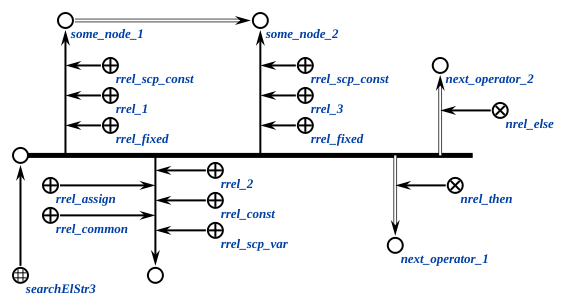
\includegraphics[scale=0.8]{images/part3/chapter_situation_management/searchElStr3_faf.png}
	\label{fig:erase_edge}
\end{figure}

\begin{figure}[H]
	\caption{SCg-текст. Пример выполнения scp-оператора удаления одноэлементной конструкции (результат выполнения scp-оператора)}
	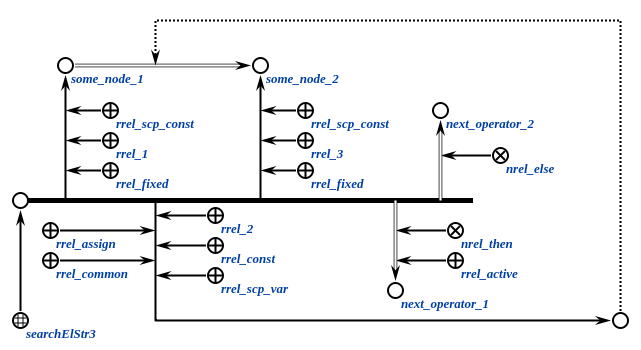
\includegraphics[scale=0.8]{images/part3/chapter_situation_management/searchElStr3_faf_2.png}
	\label{fig:erase_edge_2}
\end{figure}

\subsection{Операционная семантика Базового языка программирования ostis-систем}
\label{subsec_scp_oper}

\begin{SCn}
\begin{scnrelfromlist}{ключевой знак}
	\scnitem{Абстрактная scp-машина}
\end{scnrelfromlist}
\end{SCn}

Преимущества предложенного многоагентного подхода к обработке информации могут работать не только на платформенно-независимом уровне, но и на более низких уровнях. Так, в частности, интерпретатор \textit{Базового языка программирования ostis-систем} также предлагается строить как \textit{неатомарный абстрактный sc-агент}, обеспечивающий интерпретацию методов, описанных на \textit{Языке SCP}. Таким образом, такой интерпретатор входит в общую иерархию агентов \textit{ostis-системы} и является \textit{абстрактным sc-агентом, не реализуемым на Языке SCP}.

В общем случае вариантов реализации таких интерпретаторов может быть много. В рамках \textit{Стандарта OSTIS} один из них предлагается в качестве стандартного и называется \textit{Абстрактной scp-машиной}.

\begin{SCn}
\scnheader{Абстрактная scp-машина}
\begin{scnrelfromset}{декомпозиция абстрактного sc-агента}
	\scnitem{Абстрактный sc-агент создания scp-процессов}
	\scnitem{Абстрактный sc-агент интерпретации scp-операторов}
	\scnitem{Абстрактный sc-агент синхронизации процесса интерпретации scp-программ}
	\scnitem{Абстрактный sc-агент уничтожения scp-процессов}
	\scnitem{Абстрактный sc-агент синхронизации событий в sc-памяти и ее реализации}
	\begin{scnindent}
	\begin{scnrelfromset}{декомпозиция абстрактного sc-агента}		
		\scnitem{Абстрактный sc-агент трансляции сформированной спецификации события в sc-памяти во внутреннее представление}
		\scnitem{Абстрактный sc-агент обработки события в sc-памяти, инициирующего агентную scp-программу}
	\end{scnrelfromset}
	\end{scnindent}
\end{scnrelfromset}
\end{SCn}

Задачей \textit{Абстрактного sc-агента создания scp-процессов} является создание \textit{scp-процессов}, соответствующих заданной \textit{scp-программе}. Данный \textit{\mbox{sc-агент}} активируется при появлении в \textit{sc-памяти} \textit{инициированного действия}, принадлежащего классу \textit{действие интерпретации scp-программы}.  После проверки \textit{sc-агентом} условия инициирования выполняется создание \textit{scp-процесса} с учетов конкретных параметров интерпретации \textit{\mbox{scp-программы}}, после чего осуществляется поиск \textit{начального оператора\scnrolesign \mbox{scp-процесса}} и добавление его во множество \textit{настоящих сущностей}.

Задачей \textit{Абстрактного sc-агента интерпретации scp-операторов} является собственно интерпретация операторов \textit{scp-программы}, то есть выполнение в \textit{sc-памяти} действий, описываемых конкретным \textit{\mbox{scp-оператором}}. Данный \textit{sc-агент} активируется при появлении в \textit{sc-памяти} \textit{scp-оператора}, принадлежащего классу \textit{настоящих сущностей}. После выполнения действия, описываемого \textit{scp-оператором}, \textit{scp-оператор} добавляется во множество \textit{прошлых сущностей}. В случае когда семантика действия, описываемого \textit{\mbox{scp-оператором}}, предполагает возможность ветвления \textit{scp-программы} после выполнения данного \textit{\mbox{scp-оператора}}, то используется одно из подмножеств класса \textit{выполненных действий -- безуспешно выполненное действие} или \textit{успешно выполненное действие}.

Задачей \textit{Абстрактного sc-агента синхронизации процесса интерпретации scp-программ} является обеспечение переходов между \textit{scp-операторами} в рамках одного \textit{scp-процесса}. Данный \textit{sc-агент} активизируется при добавлении некоторого \textit{scp-оператора} во множество \textit{прошлых сущностей}. Далее осуществляется переход по \textit{sc-дуге}, принадлежащей отношению \textit{последовательность действий*} (или более частным отношениям, в случае, если \textit{\mbox{scp-оператор}} был добавлен во множество \textit{успешно выполненных действий} или \textit{безуспешно выполненных действий}). При этом очередной \textit{scp-оператор} становится \textit{настоящей сущностью} (активным \textit{scp-оператором}) в том случае, если хотя бы один \textit{scp-оператор}, связанный с ним входящими \textit{sc-дугами}, принадлежащими отношению \textit{последовательность действий*} (или более частным отношениям), стал \textit{прошлой сущностью} (или, соответственно, подмножеством прошлых сущностей). В случае, когда необходимо дождаться завершения выполнения всех предыдущих операторов, для синхронизации используется оператор класса \textit{конъюнкция предшествующих операторов}.

Задачей \textit{Абстрактного sc-агента уничтожения scp-процессов} является уничтожение \textit{scp-процесса}, то есть удаление из \textit{sc-памяти} всех \textit{sc-элементов}, его составляющих. Данный \textit{sc-агент} активируется при появлении в \textit{sc-памяти} \textit{scp-процесса}, принадлежащего множеству \textit{прошлых сущностей}.
При этом уничтожаемый \textit{scp-процесс} необязательно должен быть полностью сформирован. Необходимость уничтожения не до конца сформированного \textit{scp-процесса} может возникнуть в случае, если при создании \textit{scp-процесса} возникли проблемы, не позволяющие продолжить создание \textit{scp-процесса} и его выполнение.

Задачей \textit{Абстрактного sc-агента синхронизации событий в sc-памяти и ее реализации} является обеспечение работы \textit{неатомарных sc-агентов}, реализованных на \textit{Языке SCP}.

Задачей \textit{\textbf{Абстрактного sc-агента трансляции сформированной спецификации события в sc-памяти во внутреннее представление}} является трансляция ориентированных пар, описывающих \textit{первичное условие инициирования*} некоторого \textit{\mbox{sc-агента}} во внутреннее представление элементарных событий на уровне \textit{\mbox{sc-хранилища}}, при условии, что этот \textit{sc-агент} реализован на платформенно-независимом уровне (с использованием \textit{Языка SCP}). Условием инициирования данного \textit{sc-агента} является появление в \textit{\mbox{sc-памяти}} нового элемента множества \textit{активных sc-агентов}, для которого будет найдена и протранслирована соответствующая ориентированная пара.

Задачей \textit{Абстрактного sc-агента обработки события в sc-памяти, инициирующего агентную \mbox{scp-программу}}, является поиск \textit{агентной scp-программы}, входящей во множество \textit{программ sc-агента*} для каждого \textit{sc-агента}, первичное условие инициирования которого соответствует событию, произошедшему в \textit{sc-памяти}, а также генерация и инициирование действия, направленного на интерпретацию этой программы. В результате работы данного \textit{sc-агента} в \textit{sc-памяти} появляется \textit{инициированное действие}, принадлежащее классу \textit{действие} \textit{интерпретации scp-программы}.

\section{Решатели задач ostis-систем}
\label{sec_ps_ps}

\begin{SCn}
\begin{scnrelfromlist}{ключевое понятие}
	\scnitem{решатель задач ostis-системы}
	\scnitem{машина обработки знаний}
\end{scnrelfromlist}
\end{SCn}

С учетом того тезиса, что существуют \textit{методы} интепретации других \textit{методов} и, следовательно, иерархия \textit{методов}, а также, соответственно, иерархия \textit{навыков}, можно уточнить и понятие решателя задач, как \uline{иерархической системы навыков}. Таким образом, определим \textit{решатель задач ostis-системы} определяется как совокупность всех \textit{навыков}, которыми обладает ostis-система на текущий момент времени. 

Такой подход к уточнению архитектуры \textit{решателей задач ostis-систем} позволяет обеспечить их модифицируемость, что, в свою очередь, позволяет \textit{ostis-системе} при необходимости легко приобретать новые \textit{навыки}, модифицировать (совершенствовать) уже имеющиеся, и даже избавляться от некоторых навыков с целью повышения производительности системы. Таким образом, имеет смысл говорить не о жестко фиксированном решателе задач, который разрабатывается один раз при создании первой версии системы и далее не меняется, а о совокупности навыков, фиксированной в каждый текущий момент времени, но постоянно эволюционирующей.

\begin{SCn}
	\scnheader{решатель задач ostis-системы}
	\scnrelto{семейство подмножеств}{навык}
	\scnidtf{иерархическая система навыков, которыми обладает ostis-система}
	\scnsuperset{гибридный решатель задач ostis-системы}
	\begin{scnindent}
		\scnidtf{решатель задач ostis-системы, реализующий две и более модели решения задач}
	\end{scnindent}
	\scnsuperset{объединенный решатель задач ostis-системы}
	\begin{scnindent}
		\scnidtf{полный решатель задач ostis-системы}
		\scnidtf{интегрированный решатель задач ostis-системы}
		\scnidtf{решатель задач ostis-системы, реализующий все ее функциональные возможности, как основные, так и вспомогательные}
	\end{scnindent}
\end{SCn}

В общем случае \textit{объединенный решатель задач ostis-системы}, решает задачи, связанные с:
\begin{textitemize}
	\item обеспечением основных функциональных возможностей системы (например, решение явно сформулированных задач по требованию пользователя);
	\item обеспечением корректности и оптимизацией работы самой ostis-системы (перманентно на протяжении всего жизненного цикла ostis-системы);
	\item обеспечением повышения квалификации конечных пользователей и разработчиков ostis-системы;
	\item обеспечением автоматизации развития и управления развитием ostis-системы.
\end{textitemize}

В свою очередь, под \textit{машиной обработки знаний} будем понимать совокупность интерпретаторов всех \textit{навыков}, составляющих некоторый \textit{решатель задач}. С учетом многоагентного подхода к обработке информации, используемого в рамках \textit{Технологии OSTIS}, \textit{машина обработки знаний} представляет собой \textit{sc-агент} (чаще всего -- \textit{неатомарный sc-агент}), в состав которого входят более простые sc-агенты, обеспечивающие интерпретацию соответствующего множества \textit{методов}. Таким образом, \textit{машина обработки знаний} в общем случае представляет собой иерархическую систему \textit{sc-агентов}.

\begin{SCn}
	\scnheader{машина обработки знаний}
	\scnsubset{sc-агент}
\end{SCn}

Рассмотрим классификацию \textit{решателей задач} \textit{ostis-систем} по различным признакам.

Классификация \textit{решателей задач} \textit{ostis-систем} по типу соответствующей \textit{ostis-системы}:

\begin{SCn}
\scnheader{решатель задач ostis-системы}
\scnhaselement{Решатель задач Метасистемы OSTIS}
\scnsuperset{решатель задач вспомогательной ostis-системы}
\begin{scnindent}
	\scnsuperset{решатель задач интерфейса компьютерной системы}
	\begin{scnindent}
		\begin{scnrelfromset}{разбиение}
			\scnitem{решатель задач пользовательского интерфейса компьютерной системы}
			\scnitem{решатель задач интерфейса компьютерной системы с другими компьютерными системами}
			\scnitem{решатель задач интерфейса компьютерной системы с окружающей средой}
		\end{scnrelfromset}
	\end{scnindent}
	\scnsuperset{решатель задач ostis-подсистемы поддержки проектирования компонентов определенного класса}
	\begin{scnindent}
		\scnsuperset{решатель задач ostis-подсистемы поддержки проектирования баз знаний}
		\begin{scnindent}
			\scnsuperset{решатель задач повышения качества базы знаний}
			\begin{scnindent}
				\scnsuperset{решатель задач верификации базы знаний}
				\begin{scnindent}
					\scnsuperset{решатель задач поиска и устранения некорректностей в базе знаний}
					\scnsuperset{решатель задач поиска и устранения неполноты}
				\end{scnindent}
				\scnsuperset{решатель задач оптимизации структуры базы знаний}
				\scnsuperset{решатель задач выявления и устранения информационного мусора}
			\end{scnindent}
		\end{scnindent}
		\scnsuperset{решатель задач ostis-подсистемы поддержки проектирования решателей задач ostis-систем}
		\begin{scnindent}
			\begin{scnrelfromset}{разбиение}
				\scnitem{решатель задач ostis-подсистемы поддержки проектирования программ обработки знаний}
				\scnitem{решатель задач ostis-подсистемы поддержки проектирования агентов обработки знаний}
			\end{scnrelfromset}
		\end{scnindent}
	\end{scnindent}
	\scnsuperset{решатель задач подсистемы управления проектирования компьютерных систем и их компонентов}
\end{scnindent}
\scnsuperset{решатель задач самостоятельной ostis-системы}
\end{SCn}

Классификация \textit{решателей задач} \textit{ostis-систем} по типу интерпретируемой \textit{модели решения задач}:

\begin{SCn}
\scnheader{решатель задач ostis-системы}
\scnsuperset{решатель задач с использованием хранимых методов}
\begin{scnindent}
	\scnidtf{решатель, способный решать задачи тех классов, для которых на данный момент времени известен соответствующий метод решения}
	\scnsuperset{решатель задач на основе нейросетевых моделей}
	\scnsuperset{решатель задач на основе генетических алгоритмов}
	\scnsuperset{решатель задач на основе императивных программ}
	\begin{scnindent}
		\scnsuperset{решатель задач на основе процедурных программ}
		\scnsuperset{решатель задач на основе объектно-ориентированных программ}
	\end{scnindent}
	\scnsuperset{решатель задач на основе декларативных программ}
	\begin{scnindent}
		\scnsuperset{решатель задач на основе логических программ}
		\scnsuperset{решатель задач на основе функциональных программ}
	\end{scnindent}
\end{scnindent}
\scnsuperset{решатель задач в условиях, когда метод решения задач данного класса в текущий момент времени не известен}
\begin{scnindent}
	\scnidtf{решатель, реализующий стратегии решения задач, позволяющие породить метод решения задачи, который в текущий момент времени не известен ostis-системе}
	\scnidtf{решатель, использующий для решения задач метаметоды, соответствующие более общим классам задач по отношению к заданной}
	\scnidtf{решатель задач, позволяющий породить метод, который является частным по отношению какому-либо известному ostis-системе методу и интерпретируется соответствующей машиной обработки знаний}
	\scnsuperset{решатель, реализующий стратегию поиска путей решения задачи в глубину}
	\scnsuperset{решатель, реализующий стратегию поиска путей решения задачи в ширину}
	\scnsuperset{решатель, реализующий стратегию проб и ошибок}
	\scnsuperset{решатель, реализующий стратегию разбиения задачи на подзадачи}
	\scnsuperset{решатель, реализующий стратегию решения задач по аналогии}
	\scnsuperset{решатель, реализующий концепцию интеллектуального пакета программ}
\end{scnindent}
\end{SCn}

Отдельно выделим классификацию машин обработки знаний, которые в общем случае могут соответствовать одним и тем же фрагментам базы знаний, но при этом в совокупности с ними образовывать разные навыки и соответственно разные решатели задач:

\begin{SCn}
\scnheader{машина обработки знаний}
\scnsuperset{машина логического вывода}
\begin{scnindent}
	\scnsuperset{машина дедуктивного вывода}
	\begin{scnindent}
		\scnsuperset{машина прямого дедуктивного вывода}
		\scnsuperset{машина обратного дедуктивного вывода}
	\end{scnindent}
	\scnsuperset{машина индуктивного вывода}
	\scnsuperset{машина абдуктивного вывода}
	\scnsuperset{машина нечеткого вывода}
	\scnsuperset{машина вывода на основе логики умолчаний}
	\scnsuperset{машина логического вывода с учетом фактора времени}
\end{scnindent}
\end{SCn}

Классификация \textit{решателей задач} \textit{ostis-систем} по типу решаемой \textit{задачи} (цели решения задачи):

\begin{SCn}
\scnheader{решатель задач ostis-системы}
\scnsuperset{решатель задач информационного поиска}
\begin{scnindent}
	\begin{scnrelfromset}{разбиение}
		\scnitem{решатель задач поиска информации, удовлетворяющей заданным критериям}
		\scnitem{решатель задач поиска информации, не удовлетворяющей заданным критериям}
	\end{scnrelfromset}
\end{scnindent}
\scnsuperset{решатель явно сформулированных задач}
\begin{scnindent}
	\scnidtf{решатель задач, для которых явно сформулирована цель}
	\scnsuperset{решатель задач поиска или вычисления значений заданного множества величин}
	\scnsuperset{решатель задач установления истинности заданного логического высказывания в рамках заданной формальной теории}
	\scnsuperset{решатель задач формирования доказательства заданного высказывания в рамках заданной формальной теории}
	\scnsuperset{машина верификации ответа на указанную задачу}
	\scnsuperset{машина верификации решения указанной задачи}
	\begin{scnindent}
		\scnsuperset{машина верификации доказательства заданного высказывания в рамках заданной формальной теории}
	\end{scnindent}
\end{scnindent}
\scnsuperset{решатель задач классификации сущностей}
\begin{scnindent}
	\scnsuperset{машина соотнесения сущности с одним из заданного множества классов}
	\scnsuperset{машина разделения множества сущностей на классы по заданному множеству признаков}
\end{scnindent}
\scnsuperset{решатель задач синтеза информационных конструкций}
\begin{scnindent}
	\scnsuperset{решатель задач синтеза естественно-языковых текстов}
	\scnsuperset{решатель задач синтеза изображений}
	\scnsuperset{решатель задач синтеза сигналов}
	\begin{scnindent}
		\scnsuperset{решатель задач синтеза речи}
	\end{scnindent}
\end{scnindent}
\scnsuperset{решатель задач анализа информационных конструкций}
\begin{scnindent}
	\scnsuperset{решатель задач анализа естественно-языковых текстов}
	\begin{scnindent}
		\scnsuperset{решатель задач понимания естественно-языковых текстов}
		\scnsuperset{решатель задач верификации естественно-языковых текстов}
	\end{scnindent}
	\scnsuperset{решатель задач анализа изображений}
	\begin{scnindent}
		\scnsuperset{решатель задач сегментации изображений}
		\scnsuperset{решатель задач понимания изображений}
	\end{scnindent}
	\scnsuperset{решатель задач анализа сигналов}
	\begin{scnindent}
		\scnsuperset{решатель задач анализа речи}
		\begin{scnindent}
			\scnsuperset{решатель задач понимания речи}
		\end{scnindent}
	\end{scnindent}
\end{scnindent}
\end{SCn}

\section{Принципы решения задач распределенными коллективами ostis-систем}
\label{sec_ps_collective}

Разработка \textit{решателей задач} \textit{интеллектуальных систем} на настоящий момент как правило рассматриваются в контексте одиночных (самостоятельных) интеллектуальных систем, функционирующих в некоторой среде (частью которой является и пользователь, если он есть). В то же время очевидна тенденция современных информационных технологий к переходу от одиночных систем к коллективам распределенных взаимодействующих компьютерных систем, в частности, к распределенному хранению данных и распределенным вычислениям. В случае интеллектуальных компьютерных систем важнейшим свойством систем, входящих в такие коллективы, становится \uline{\textit{интероперабельность}}, то есть способность системы к согласованному взаимодействию с другими подобными системами с целью решения каких-либо задач. Таким образом, особо актуальным является переход от разработки \textit{решателей задач} отдельно взятых интеллектуальных систем к решателям задач взаимодействующих \textit{интероперабельных интеллектуальных систем}, включая разработку принципов решения задач в таких распределенных коллективах с учетом решения всех обозначенных выше проблем. Важно отметить, что полностью отказаться от распределенности при решении задач даже в сравнительно простых прикладных системах нельзя, поскольку часто интеллектуальные системы вынуждены использовать различные датчики и эффекторы, которые с точки зрения общей архитектуры являются некоторыми внешними модулями (внешними агентами) и, таким образом, привносят распределенность в общую архитектуру системы.

Для решения данной проблемы предлагается рассмотреть такую систему взаимодействующих \textit{интеллектуальных компьютерных систем} как \textit{многоагентную систему} и уточнить принцип поведения \textit{агентов} в такой системе.

Таким образом, можно говорить о двух видах многоагентных систем в рамках \textit{Технологии OSTIS}:
\begin{textitemize}
	\item внутренняя система sc-агентов над общей sc-памятью в рамках некоторой ostis-системы;
	\item распределенная система ostis-систем в рамках Экосистемы OSTIS.
\end{textitemize}	

В обоих случаях можно говорить об \myuline{иерархии агентов}:
\begin{textitemize}
	\item в рамках внутренней системы sc-агентов выделяются \textit{атомарные абстрактные sc-агенты} и \textit{неатомарные абстрактные sc-агенты}, кроме того существует иерархия sc-агентов с точки зрения языка интерпретации методов (см. \textit{\ref{sec_ps_agents} \nameref{sec_ps_agents}});
	\item в рамках \textit{Экосистемы OSTIS} выделяются как \textit{индивидуальные ostis-системы}, так и \textit{коллективные ostis-системы}, которые в свою очередь могут состоять как из \textit{индивидуальных ostis-систем}, так и \textit{коллективных ostis-систем} (см. \textit{\ref{sec_sem_compatible_os}~\nameref{sec_sem_compatible_os}}).
\end{textitemize}	

Ключевым отличием \textit{распределенной системы ostis-систем} от \textit{внутренней системы sc-агентов} в рамках \textit{индивидуальной ostis-системы} является отсутствие общей памяти, хранящей общую для всех \textit{sc-агентов} \textit{базу знаний} и выступающей в роли среды для коммуникации \textit{sc-агентов}. В общем случае в качестве средства коммуникации между агентами в рамках выделенных систем агентов может использоваться:
\begin{textitemize}
	\item Общая нераспределенная (монолитная) память, как в случае \textit{sc-агентов} над \textit{sc-памятью};
	\item Общая распределенная память. В этом случае с логической точки зрения агенты могут считать, что по-прежнему работают над общей памятью, в рамках которой хранится вся доступная база знаний, однако реально \textit{база знаний} будет распределена между несколькими \textit{ostis-системами} и выполняемые преобразования должны будут синхронизироваться между этими ostis-системами;
	\item Специализированные каналы связи. Очевидно, что при решении задачи в распределенном коллективе \textit{ostis-систем} должны существовать языковые и технические средства, позволяющие осуществлять передачу сообщений от одной \textit{ostis-системы} к другой.
\end{textitemize}

Все перечисленные средства коммуникации в зависимости от класса решаемой задачи, требуемых для ее решения \textit{знаний} и \textit{навыков}, а также существующего (доступного) в данный момент набора \textit{ostis-систем} могут \myuline{комбинироваться}.

В основу решения задач в рамках \textit{распределенного коллектива ostis-систем} предлагается положить идею максимально возможной \myuline{унификации} и \myuline{конвергенции} принципов решения задач в рамках \textit{индивидуальной ostis-системы} и \textit{распределенного коллектива ostis-систем}. Такой подход обладает следующим важным достоинством: если общие принципы решения задач не зависят от того, какой конкретно набор \textit{ostis-систе}м участвует в решении той или иной задачи, то становится возможным легко переходить от \textit{индивидуальной ostis-системы} к \textit{распределенному коллективу ostis-систем} при ее усложнении без необходимости существенно пересматривать коллектив \textit{агентов}, входящих в состав такой \textit{ostis-системы} и заново продумывать используемый подход к решению задач того или иного класса. Для перехода от \textit{индивидуальной ostis-системы} к \textit{коллективной ostis-системе} достаточно выполнить следующие шаги:
\begin{textitemize}
	\item Разделить множество классов задач, решаемых данной \textit{ostis-системой}, на семейство подмножеств, каждое из которых обладает некоторой логической целостностью, критерии которой в общем случае определяются разработчиком. При этом указанные подмножества могут пересекаться, но при объединении должны давать исходное множество, таким образом необходимо построить одно из возможных \textit{покрытий*} для множества классов задач, решаемых данной \textit{ostis-системой};
	\item Для каждого из выделенных подмножеств необходимо сформировать множество \textit{знаний} и \textit{навыков}, необходимых для решения задач данного множества классов. При этом в общем случае может оказаться необходимым пересмотр иерархии навыков и соответствующих им sc-агентов, в частности, преобразование некоторых атомарных sc-агентов в неатомарные. Теоретически избежать такой ситуации невозможно, однако подобные ситуации можно практически исключить на этапе проектирования решателей задач индивидуальных ostis-систем, делая иерархию агентов достаточно глубокой и ставя в соответствие \textit{атомарным sc-агентам} такие \textit{классы задач}, разделение которых на подклассы с практической точки зрения не имеет смысла. 
	
	\vspace{-0.5\baselineskip}
	Аналогичная ситуация может возникнуть и при выделении фрагментов \textit{базы знаний}. В этом случае может потребоваться пересмотр иерархии \textit{предметных областей} и \textit{онтологий} и, возможно, выделение новых предметных областей. Как и в случае с \textit{решателями задач}, избежать такой ситуации на практике возможно в случае, если иерархия предметных областей будет достаточно глубокой для того, чтобы выделение более частных предметных областей было практически нецелесообразным;
	\vspace{0.5\baselineskip}
	
	\item Каждое сформированное таким образом множество знаний и навыков становится соответственно базой знаний и решателем задач новой ostis-системы, которая будет способна реализовать только часть функциональных возможностей исходной ostis-системы. 
\end{textitemize}

Такое разделение может выполняться итерационно и для полученных \textit{ostis-систем} в общем случае неограниченное количество раз, создавая на каждой итерации новое "поколение"{} ostis-систем, полученное путем декомпозиции исходной \textit{ostis-системы}. 

Таким образом, предлагаемая идея унификации принципов решения задач в \textit{ostis-системах} любого рода позволяет 
\begin{textitemize}
	\item с практической точки зрения снять ограничение на расширение функциональных возможностей (обучение) не только \textit{индивидуальной ostis-системы}, но и \textit{коллективной ostis-системы}, позволяя, таким образом, постоянно наращивать функциональные возможности \textit{Экосистемы OSTIS} в целом. 
	\item с теоретической (архитектурной) точки зрения говорить о \myuline{фрактальном} характере не только внутренней организации \textit{ostis-систем} но и \textit{коллективов ostis-систем}, что, в свою очередь, позволяет обеспечить возможность наследования и других принципов построения \textit{индивидуальных ostis-систем} в \textit{распределенных коллективах ostis-систем}, включая, например, методику проектирования \textit{ostis-систем} и их компонентов и соответствующие средства, а также принципы синхронизации соответствующих sc-агентам параллельных \textit{информационных процессов}.
\end{textitemize}	

В основе взаимодействия \textit{sc-агентов} в рамках \textit{индивидуальной ostis-системы} лежит уточненный принцип "доски объявлений"{} при котором агенты взаимодействуют посредством общей для них sc-памяти (см. \textit{\ref{subsec_ps_proposed_approach} \nameref{subsec_ps_proposed_approach}}). Для реализации той же идеи в случае \textit{распределенной коллективной ostis-системы} необходимо выбрать какую-либо sc-память для выполнения данной роли. При решении задач в \textit{распределенном коллективе ostis-систем} возможны два варианта организации взаимодействия \textit{агентов} (которыми являются и сами \textit{ostis-системы}):
\begin{textitemize}
	\item Если решаемая задача достаточно сложная и требует частого обращения к нескольким отдельным \textit{ostis-системам}, то целесообразно путем объединения раздельных ostis-систем создать \textit{временную ostis-систему}, где все sc-агенты, входившие в состав исходных \textit{ostis-систем}, становятся внутренними, и принципы организации их взаимодействия известны. В этом случае существенно снижаются затраты на решение задачи, но появляются накладные расходы на создание таких \textit{временных ostis-систем}. Таким образом, необходимо отдельно разработать критерии на основании которых будет приниматься решение о целесообразности такого объединения. Отметим, что для того, чтобы иметь возможность сохранить результат и ход решения задачи для последующего применения целесообразно осуществлять объединение \textit{ostis-систем} на базе одной из \textit{ostis-систем}, входящих в такое объединение, а не создавать совершенно новую \textit{ostis-систему}. При этом в такую систему будут копироваться знания и навыки из объединяемых систем, а сами эти объединяемые системы могут вообще никак не меняться. Тогда после решения задачи из исходной \textit{ostis-системы} необходимо будет исключить те \textit{навыки} и \textit{знания}, которые были нужны только для решения данной задачи.
	
	Важно отметить, что описанная интеграция \textit{ostis-систем} благодаря особенностям их архитектуры выполняется значительно проще, чем в других компьютерных системах, поскольку принципы построения и баз знаний, и \textit{решателей задач} \textit{ostis-систем} изначально предполагают возможность неограниченного расширения имеющихся в системе знаний и навыков без необходимости внесения изменений в уже имеющуюся \textit{базу знаний} и \textit{решатель задач}. Таким образом, интеграция двух ostis-систем при условии их семантической совместимости сводится к обычному теоретико-множественному объединению их \textit{баз знаний} и \textit{решаталей задач} и последующему исключению продублированных компонентов. Благодаря этому создание таких временных ostis-систем может выполняться \myuline{автоматически}, что делает применение такого подхода к организации решения задач целесообразным во многих случаях.

	\item Другой возможный вариант предполагает, что в качестве среды для взаимодействия \textit{sc-агентов} (как внешних, так и внутренних, внешняя \textit{ostis-система} с точки зрения процесса решения задачи также рассматривается как \textit{sc-агент}) выбирается \textit{sc-память} одной из \textit{ostis-систем}, входящих в состав \textit{коллектива ostis-систем}. Предлагаются следующие критерии выбора этой sc-памяти:
	\begin{textitemize}
		\item Если задача решается неоднократно в рамках некоторого \textit{ostis-сообщества} (\textit{сообщества ostis-систем} и их пользователей, см. \textit{\ref{sec_ecosystem_structure}~\nameref{sec_ecosystem_structure}}), то для координации действий \textit{sc-агентов} выбирается \textit{sc-память} \textit{корпоративной ostis-системы} для данного \textit{ostis-сообщества};
		\item Если \textit{коллектив ostis-систем} для решения данной задачи формируется временно (разово), то для координации действий \textit{sc-агентов} выбирается \textit{sc-память} той \textit{ostis-системы}, которая инициировала решение данной задач.
	\end{textitemize}
	\vspace{-\baselineskip}
	Недостатком данного варианта является наличие затрат на коммуникацию между \textit{ostis-системами}. Если по каким-либо причинам эти затраты велики (например, из-за низкого качества соединения между системами), то более целесообразно использовать первый из предложенных вариантов.
\end{textitemize}

В любом из предложенных вариантов в конечном итоге определяется некоторая конкретная sc-память, которая становится средой для взаимодействия агентов, осуществляющих решение задачи, по изложенным в \textit{\ref{subsec_ps_proposed_approach} \nameref{subsec_ps_proposed_approach}} принципам. Тогда можно уточнить понятие \textit{sc-агента} как компонента решателя задач в контексте распределенного решения задач \textit{коллективом ostis-систем} и считать sc-агентом не только компонент \textit{решателя задач индивидуальной ostis-системы}, но и любую ostis-систему, входящую в постоянный либо временный \textit{коллектив ostis-систем}, решающих какие-либо задачи, поскольку принципы взаимодействия \textit{ostis-систем} в таком коллективе полностью совпадают с принципами взаимодействия \textit{sc-агентов} в составе \textit{решателя задач} \textit{индивидуальной ostis-системы}.

Таким образом, можно говорить о фрактальной иерархической структуре распределенного \textit{гибридного решателя задач}, в рамках которой выделяется два варианта иерархии \textit{sc-агентов}:
\begin{textitemize}
	\item Иерархия sc-агентов с точки зрения уровня \textit{языков представления методов}, на которых представлены соответствующие этим sc-агентам методы. В рамках этой иерархии в свою очередь можно выделить три уровня, имеющих важные отличия:
	\begin{textitemize}
		\item Уровень \textit{sc-агентов} \textit{ostis-платформы}, обеспечивающий интерпретацию методов платформенно-независимого уровня в рамках \textit{индивидуальной ostis-системы}, в рамках которого может выделяться иерархия языков представления методов уровня ostis-платформы и соответствующих средств их интерпретации;
		\item Уровень \textit{платформенно-независимых sc-агентов} в рамках \textit{индивидуальной ostis-системы}, в рамках которого может выделяться иерархия платформенно-независимых языков представления методов;
		\item Уровень \textit{распределенных коллективов ostis-систем}, на котором также можно говорить о \textit{языках представления методов} и их иерархии, но при этом в общем случае даже отдельные методы могут физически храниться распределенно в разных ostis-системах. Например, можно говорить о \textit{языке представления методов} для финансовой деятельности крупных предприятий, но при этом целесообразно выделять подъязыки для описания деятельности отделов различных категорий и иметь отдельные ostis-системы для обслуживания каждого из отделов.
	\end{textitemize}	
	\item Иерархия sc-агентов с точки зрения атомарности/неатомарности в рамках \myuline{одного} \textit{языка представления методов}. Формирование такой иерархии может быть целесообразным на любом уровне языка \textit{языка представления методов} и приводит к выделению:
	\begin{textitemize}
		\item \textit{атомарных платформенно-зависимых sc-агентов} и \textit{неатомарных платформенно-зависимых sc-агентов} на уровне \textit{ostis-платформы};
		\item \textit{атомарных платформенно-независимых sc-агентов} и \textit{неатомарных платформенно-независимых sc-агентов} на платформенно-независимом уровне в рамках индивидуальной ostis-системы;
		\item \textit{индивидуальных ostis-систем} и \textit{коллективных ostis-систем} на уровне решения задач в рамках \textit{Экосистемы OSTIS}.
	\end{textitemize}	
\end{textitemize}
	
Дальнейшее развитие представленных принципов решения задач распределенными коллективами ostis-систем предполагает:
\begin{textitemize}
	\item Разработку формальных критериев для оценки целесообразности или нецелесообразности формирования временных индивидуальных ostis-систем;
	\item Разработку языка и принципов обмена сообщениями между ostis-системами, входящими в коллектив ostis-систем, решающий какую-либо задачу. Несмотря на то, что с логической точки зрения каждая ostis-система трактуется как sc-агент и принципы их взаимодействия остаются теми же, реализация, например, возможности реагирования на события в базе знаний и внесения изменений в эту базу знаний для внутренних sc-агентов и внешних ostis-систем будет отличаться и требует уточнения.
\end{textitemize}

\section{Актуальные проблемы и перспективы развития технологий разработки гибридных решателей задач}
\markboth{Перспективы развития технологий разработки гибридных решателей задач}{Перспективы развития технологий разработки гибридных решателей задач}
\label{sec_ps_future}

В данной главе был детально рассмотрен подход к построению \textit{решателей задач}, позволяющий решить ряд фундаментальных проблем в области построения \textit{решателей задач}, таких как обеспечение совместимости различных \textit{решателей задач} и их компонентов, а также обеспечение обучаемости (модифицируемости и рефлексивности) самих \textit{решателей задач}. В то же время существует существует ряд проблем, остающихся актуальными и требующих решения.

Первая проблема связана с отсутствием достаточно строгой формализованной классификации задач, решаемых интеллектуальными системами, отсутствием унификации описания задач и классов задач, описания целей, хода и результата решения задачи, методов решения задач, связей между классами задач и методами решения задач данного класса. Решение данной проблемы, с одной стороны, позволит обеспечить возможность глубокой интеграции всевозможных \textit{моделей решения задач} различных классов и возможность облегчить процесс интеграции новых моделей решения задач в интеллектуальную систему, а с другой стороны, станет предпосылкой для решения других проблем, описанных ниже.

Вторая проблема заключается в том, что на настоящий момент основное внимание в области разработки \textit{гибридных решателей задач} уделено снижению трудоемкости интеграции различных компонентов решателя задач в \textit{интеллектуальную систему} и реализации возможности накопления многократно используемых компонентов \textit{решателей задач}, однако в общем случае не говорится о том, как конкретно \textit{интеллектуальная система} будет применять те или иные компоненты при решении задач конкретных классов. Таким образом, построение общего плана решения задачи, то есть выбор методов решения задач, определение порядка их применения и выбор исходных данных (аргументов) для применения того или иного метода, фактически определяется разработчиком на этапе проектирования системы или на этапе ее эволюции в процессе эксплуатации. Предпосылкой для решения данной проблемы является решение ранее рассмотренной проблемы унификации представления задач различных классов и методов их решения. Решение же рассматриваемой проблемы предполагает разработку комплекса \textit{стратегий решения задач} (или \textit{метаметодов решения задач}), которые позволят \textit{интеллектуальной системе} самостоятельно формировать план решения задачи с учетом имеющихся в системе методов решения задач и, при возможности, даже запрашивать недостающие для решения задачи компоненты в соответствующих библиотеках. Следует отметить, что попытки разработки универсальных высокоуровневых подходов к решению задач предпринимались еще на заре развития \textit{Искусственного интеллекта}, в 1950-60ые годы, однако не увенчались успехов и вскоре прекратились. Во многом это связано с отсутствием на тот момент унифицированных моделей представления и обработки знаний, которые в настоящий момент предлагаются в рамках \textit{Технологии OSTIS}. 

Еще одна актуальная проблема, тесно связанная с рассмотренными выше, заключается в том, что интеллектуальные системы часто вынуждены решать задачи в условиях так называемых не-факторов, то есть неполноты описания задачи и возможных путей ее решения, нечеткости и некорректности имеющихся знаний, отсутствия критериев для оценки оптимальности полученного решения и т.д. (см. \scncite{Narinjani2004}). В особенности это актуально при решении поведенческих задач, связанных с изменением состояния объектов среды, внешней по отношению к интеллектуальной системе. Для решения задач в подобных условиях интеллектуальная система должна не только обладать достаточным набором компонентов решателя задач, реализующих модели решения задач в условиях наличия не-факторов (нечеткие логические модели, модели машинного обучения, генетические алгоритмы и так далее), но и реализовывать \textit{стратегии решения задач}, которые бы позволили принимать решения и формировать \textit{план решения задачи} в такого рода условиях.

Рассмотренные проблемы связаны в первую очередь с процессом решения конкретной задачи интеллектуальной системой. В то же время очевидно, что в каждый момент времени интеллектуальная система вынуждена параллельно решать несколько задач, которые могут быть связаны как с непосредственным функциональным назначением системы, так и с обеспечением жизнедеятельности и эволюции самой системы. Во втором случае имеются в виду, в частности, задачи, связанные с актуализацией имеющихся у нее сведений о внешнем мире, поиском и устранением ошибок в базе знаний, оптимизацией структуры \textit{базы знаний} и \textit{решателя задач} системы, поиском и устранением информационного мусора и многие другие. При этом разные задачи могут иметь разный приоритет, который может меняться в зависимости от ситуации даже в процессе ее решения. В то же время, в ситуации, когда априори не известно, какой из возможных способов решения задачи окажется наиболее эффективным, может оказаться целесообразным параллельное использование нескольких подходов к решению одной и той же задачи. Таким образом, актуальной является проблема организации управления информационными процессами решения задач в интеллектуальной системе и взаимодействия параллельно выполняемых информационных процессов с учетом приоритетности процессов, возможности отслеживать текущее состояние \textit{информационных процессов}, порождать, приостанавливать и уничтожать информационные процессы. Для решения данной проблемы целесообразно заимствовать решения, широко используемые в традиционных компьютерных системах, в частности, реализуемые в современных операционных системах, и адаптировать их к специфике решения задач в интеллектуальных системах. Важно отметить, что реализация модели управления информационными процессами на основе общих унифицированных моделей обработки информации, предлагаемых в рамках \textit{Технологии OSTIS}, позволит сделать одни информационные процессы объектом анализа других информационных процессов, что, в свою очередь, даст возможность анализировать ход решения задачи непосредственно в процессе решения, оценивать эффективность тех или иных методов решения задач, накапливать наиболее удачные решения для применения в дальнейшем для решения аналогичных задач и многое другое.

Решение перечисленных проблем позволит разработать принципиально новую иерархическую модель \textit{гибридного решателя задач}, обладающую рядом существенных преимуществ, которая, в свою очередь, должна будет интерпретироваться на каких-либо платформах. Без унификации требований к \textit{ostis-платформе} и четкого разделения платформенно-независимой модели системы (и в частности решателя) и \textit{ostis-платформы} невозможно говорить о реализации модели \textit{решателя задач}, реализующей рассмотренные выше идеи. Это приведет к необходимости дублирования одних и тех же компонентов модели для разных платформ, значительно усложнит интеграцию компонентов \textit{решателя задач}, поскольку потребует учета при такой интеграции особенностей каждой \textit{ostis-платформы}. Кроме того, четкое разделение уровня модели системы и уровня \textit{ostis-платформы} даст возможность независимо друг от друга развивать различные платформы и модели интеллектуальных систем. Таким образом, предлагается сформулировать унифицированные требования к \textit{ostis-платформе}, а также построить общую модель такой \textit{ostis-платформы}, удовлетворяющую указанным требованиям. Более подробно такая модель \textit{ostis-платформы} рассмотрена в \textit{Главе \ref{chapter_interpreter}~\nameref{chapter_interpreter}}.

С другой стороны, как уже было сказано, \textit{решатель задач} представляет собой сложную систему, ориентированную на работу со знаниями, а не с данными, в отличие от современных программных систем, в которых изначально известно, где конкретно локализованы нужные данные и в какой форме они представлены. В связи с этим, применение для разработки интеллектуальных систем современных программно-аппаратных платформ, ориентированных на адресный доступ к хранящимся в памяти данным, не всегда оказывается эффективным, поскольку при разработке интеллектуальных систем фактически приходится моделировать нелинейную память на базе линейной. Повышение эффективности решения задач интеллектуальными системами требует разработки специализированных платформ, в том числе аппаратных, ориентированных на унифицированные семантические модели представления и обработки информации. В качестве основы для таких разработок предлагается использовать предложенную в рамках \textit{Технологии OSTIS} общую концепцию \textit{ассоциативного семантического компьютера}, \textit{семантической памяти} и базового языка программирования, ориентированного на обработку информации в такой памяти, и дополнить их идеями \textit{волновых языков программирования}, \textit{инсерционного программирования} и других подходов, направленными на повышение эффективности обработки знаний, в том числе на аппаратном уровне. Более подробно концепция \textit{ассоциативного семантического компьютера} рассматривается в \textit{Главе \ref{chapter_computers}~\nameref{chapter_computers}}. 

В случае же распределенного коллектива интеллектуальных систем важнейшей проблемой является не просто обеспечение возможности решения задач таким коллективом в текущий момент времени, а перманентная поддержка семантической совместимости и, как следствие, интероперабельности систем, входящих в такой коллектив на протяжении всего их жизненного цикла. Очевидно, что каждая из систем, входящих в такой коллектив, и, соответственно, ее \textit{решатель задач} может эволюционировать независимо от других систем, но при этом всегда должна сохраняться \textit{интероперабельность} между системами, в противном случае решение задач в таком коллективе станет невозможным. Решение данной проблемы предполагает разработку методов перманентного анализа \textit{семантической совместимости} распределенного коллектива взаимодействующих интеллектуальных систем, выявления и устранения проблем.

Для решения указанных проблем предлагается на основе подхода к построению гибридных решателей задач, рассмотренного в данной главе, разработать:
\begin{textitemize}
	\item Комплексную онтологию действий, задач и методов их решения, а также онтологию \textit{гибридных решателей задач} на основе которой уточнить понятие решателя и его архитектуру. В \textit{Главе \ref{chapter_actions}~\nameref{chapter_actions}} представлена первая версия \textit{Глобальной предметной области действий и задач и соответствующая ей онтологии методов и технологий}, на ее основе предлагается разработать комплексную онтологию действий и задач, решаемых \textit{ostis-системами};
	\item Комплекс унифицированных обобщенных стратегий (метаметодов) решения задач в интеллектуальных системах, позволяющий интеллектуальной системе самостоятельно формировать план решения задачи с учетом имеющихся в системе \textit{методов решения задач}. В основу разрабатываемых стратегий кроме опыта аналогичных работ предлагается внести также некоторые общеметодологические идеи, связанные с \textit{Теорией бихевиоризма} и набирающими популярность идеями ее применения в информатике (см. \scncite{Cao2010}, \scncite{Cao2014}, \scncite{Pavel2015}), ТРИЗ (см. \scncite{Altshuller2010}), а также \textit{СМД-методологией}, предложенной школой Г. П. Щедровицкого (см. \scncite{Shhedrovickij1995});
	\item Онтологическую модель формирования плана решения задачи и управления процессом решения задач в гибридных решателях задач в условиях различных не-факторов и отсутствия четких критериев оценки оптимальности полученного решения. Для разработки данной модели предлагается адаптировать теорию \textit{ситуационного управления} (см. \scncite{Pospelov1986}), и реализовать ее в контексте семантической теории \textit{решателей задач}, разрабатываемой в рамках \textit{Технологии OSTIS};
	\item Комплексную онтологическую модель управления информационными процессами решения задач в интеллектуальных системах, построенных на базе унифицированных семантических моделей представления и обработки информации;
	\item Онтологическую модель платформы интерпретации унифицированных семантических моделей представления и обработки информации (\textit{ostis-платформы}). Первая версия данной модели рассмотрена в \textit{Главе \ref{chapter_interpreter} \nameref{chapter_interpreter}};
	\item Комплексную иерархическую модель \textit{гибридного решателя задач}, основанную на многоагентном подходе и учитывающую необходимость решения задач как в рамках одиночных интеллектуальных систем, так и в рамках \myuline{распределенных} \myuline{коллективов интероперабельных} \myuline{интеллектуальных систем};
	\item Комплекс методов анализа качества \textit{гибридных решателей задач} и их компонентов;
	\item Комплекс методик и средств поддержки проектирования \textit{гибридных решателей задач}. Первая версия такой методики и средств рассмотрена в \textit{Главе \ref{chapter_ps_design} \nameref{chapter_ps_design}}.
\end{textitemize}

\section*{Заключение к Главе \ref{chapter_situation_management}}

В данной главе рассмотрены актуальные на сегодняшний день проблемы в области разработки \textit{гибридных решателей задач} и предложен общий подход к построению \textit{гибридных решателей задач}, который решает такие проблемы, как обеспечение совместимости и модифицируемости \textit{решателей задач}, а также создает предпосылки к решению других актуальных проблем, подробнее рассмотренных в \textit{\ref{sec_ps_future} \nameref{sec_ps_future}}.

Сформулируем ряд конкретных направлений развития предложенных в данной главе подходов:

\begin{textitemize}
	\item Более тесно и полно интегрировать идеи ситуационного управления в предлагаемый подход;
	\item Доработать предложенный механизм блокировок, в частности, минимизировать число классов блокировок, учесть и реализовать идеи реализации lock-free алгоритмов;
	\item Исключить необходимость введения \textit{sc-метаагентов} и \textit{scp-метапрограмм}.
	\item Доработать \textit{Язык SCP} до того, чтобы иметь возможность описывать в рамках \textit{scp-программ} рецепторное и эффекторное взаимодействие \textit{ostis-систем}.
	\item При разработке \textit{Абстрактной scp-машины} учесть принципы построения волновых языков программирования (см. \scncite{Sapatyj1986}, \scncite{Moldovan1985}) и идеи инсерционного программирования и моделирования (см. \scncite{Letichevskij2003}, \scncite{Letichevskij2012}).
\end{textitemize}

%%%%%%%%%%%%%%%%%%%%%%%%% referenc.tex %%%%%%%%%%%%%%%%%%%%%%%%%%%%%%
% sample references
% %
% Use this file as a template for your own input.
%
%%%%%%%%%%%%%%%%%%%%%%%% Springer-Verlag %%%%%%%%%%%%%%%%%%%%%%%%%%
%
% BibTeX users please use
% \bibliographystyle{}
% \bibliography{}
%
\biblstarthook{In view of the parallel print and (chapter-wise) online publication of your book at \url{www.springerlink.com} it has been decided that -- as a genreral rule --  references should be sorted chapter-wise and placed at the end of the individual chapters. However, upon agreement with your contact at Springer you may list your references in a single seperate chapter at the end of your book. Deactivate the class option \texttt{sectrefs} and the \texttt{thebibliography} environment will be put out as a chapter of its own.\\\indent
References may be \textit{cited} in the text either by number (preferred) or by author/year.\footnote{Make sure that all references from the list are cited in the text. Those not cited should be moved to a separate \textit{Further Reading} section or chapter.} If the citatiion in the text is numbered, the reference list should be arranged in ascending order. If the citation in the text is author/year, the reference list should be \textit{sorted} alphabetically and if there are several works by the same author, the following order should be used:
\begin{enumerate}
\item all works by the author alone, ordered chronologically by year of publication
\item all works by the author with a coauthor, ordered alphabetically by coauthor
\item all works by the author with several coauthors, ordered chronologically by year of publication.
\end{enumerate}
The \textit{styling} of references\footnote{Always use the standard abbreviation of a journal's name according to the ISSN \textit{List of Title Word Abbreviations}, see \url{http://www.issn.org/en/node/344}} depends on the subject of your book:
\begin{itemize}
\item The \textit{two} recommended styles for references in books on \textit{mathematical, physical, statistical and computer sciences} are depicted in ~\cite{science-contrib, science-online, science-mono, science-journal, science-DOI} and ~\cite{phys-online, phys-mono, phys-journal, phys-DOI, phys-contrib}.
\item Examples of the most commonly used reference style in books on \textit{Psychology, Social Sciences} are~\cite{psysoc-mono, psysoc-online,psysoc-journal, psysoc-contrib, psysoc-DOI}.
\item Examples for references in books on \textit{Humanities, Linguistics, Philosophy} are~\cite{humlinphil-journal, humlinphil-contrib, humlinphil-mono, humlinphil-online, humlinphil-DOI}.
\item Examples of the basic Springer style used in publications on a wide range of subjects such as \textit{Computer Science, Economics, Engineering, Geosciences, Life Sciences, Medicine, Biomedicine} are ~\cite{basic-contrib, basic-online, basic-journal, basic-DOI, basic-mono}. 
\end{itemize}
}

\begin{thebibliography}{99.}%
% and use \bibitem to create references.
%
% Use the following syntax and markup for your references if 
% the subject of your book is from the field 
% "Mathematics, Physics, Statistics, Computer Science"
%
% Contribution 
\bibitem{science-contrib} Broy, M.: Software engineering --- from auxiliary to key technologies. In: Broy, M., Dener, E. (eds.) Software Pioneers, pp. 10-13. Springer, Heidelberg (2002)
%
% Online Document
\bibitem{science-online} Dod, J.: Effective substances. In: The Dictionary of Substances and Their Effects. Royal Society of Chemistry (1999) Available via DIALOG. \\
\url{http://www.rsc.org/dose/title of subordinate document. Cited 15 Jan 1999}
%
% Monograph
\bibitem{science-mono} Geddes, K.O., Czapor, S.R., Labahn, G.: Algorithms for Computer Algebra. Kluwer, Boston (1992) 
%
% Journal article
\bibitem{science-journal} Hamburger, C.: Quasimonotonicity, regularity and duality for nonlinear systems of partial differential equations. Ann. Mat. Pura. Appl. \textbf{169}, 321--354 (1995)
%
% Journal article by DOI
\bibitem{science-DOI} Slifka, M.K., Whitton, J.L.: Clinical implications of dysregulated cytokine production. J. Mol. Med. (2000) doi: 10.1007/s001090000086 
%
\bigskip

% Use the following (APS) syntax and markup for your references if 
% the subject of your book is from the field 
% "Mathematics, Physics, Statistics, Computer Science"
%
% Online Document
\bibitem{phys-online} J. Dod, in \textit{The Dictionary of Substances and Their Effects}, Royal Society of Chemistry. (Available via DIALOG, 1999), 
\url{http://www.rsc.org/dose/title of subordinate document. Cited 15 Jan 1999}
%
% Monograph
\bibitem{phys-mono} H. Ibach, H. L\"uth, \textit{Solid-State Physics}, 2nd edn. (Springer, New York, 1996), pp. 45-56 
%
% Journal article
\bibitem{phys-journal} S. Preuss, A. Demchuk Jr., M. Stuke, Appl. Phys. A \textbf{61}
%
% Journal article by DOI
\bibitem{phys-DOI} M.K. Slifka, J.L. Whitton, J. Mol. Med., doi: 10.1007/s001090000086
%
% Contribution 
\bibitem{phys-contrib} S.E. Smith, in \textit{Neuromuscular Junction}, ed. by E. Zaimis. Handbook of Experimental Pharmacology, vol 42 (Springer, Heidelberg, 1976), p. 593
%
\bigskip
%
% Use the following syntax and markup for your references if 
% the subject of your book is from the field 
% "Psychology, Social Sciences"
%
%
% Monograph
\bibitem{psysoc-mono} Calfee, R.~C., \& Valencia, R.~R. (1991). \textit{APA guide to preparing manuscripts for journal publication.} Washington, DC: American Psychological Association.
%
% Online Document
\bibitem{psysoc-online} Dod, J. (1999). Effective substances. In: The dictionary of substances and their effects. Royal Society of Chemistry. Available via DIALOG. \\
\url{http://www.rsc.org/dose/Effective substances.} Cited 15 Jan 1999.
%
% Journal article
\bibitem{psysoc-journal} Harris, M., Karper, E., Stacks, G., Hoffman, D., DeNiro, R., Cruz, P., et al. (2001). Writing labs and the Hollywood connection. \textit{J Film} Writing, 44(3), 213--245.
%
% Contribution 
\bibitem{psysoc-contrib} O'Neil, J.~M., \& Egan, J. (1992). Men's and women's gender role journeys: Metaphor for healing, transition, and transformation. In B.~R. Wainrig (Ed.), \textit{Gender issues across the life cycle} (pp. 107--123). New York: Springer.
%
% Journal article by DOI
\bibitem{psysoc-DOI}Kreger, M., Brindis, C.D., Manuel, D.M., Sassoubre, L. (2007). Lessons learned in systems change initiatives: benchmarks and indicators. \textit{American Journal of Community Psychology}, doi: 10.1007/s10464-007-9108-14.
%
%
% Use the following syntax and markup for your references if 
% the subject of your book is from the field 
% "Humanities, Linguistics, Philosophy"
%
\bigskip
%
% Journal article
\bibitem{humlinphil-journal} Alber John, Daniel C. O'Connell, and Sabine Kowal. 2002. Personal perspective in TV interviews. \textit{Pragmatics} 12:257--271
%
% Contribution 
\bibitem{humlinphil-contrib} Cameron, Deborah. 1997. Theoretical debates in feminist linguistics: Questions of sex and gender. In \textit{Gender and discourse}, ed. Ruth Wodak, 99--119. London: Sage Publications.
%
% Monograph
\bibitem{humlinphil-mono} Cameron, Deborah. 1985. \textit{Feminism and linguistic theory.} New York: St. Martin's Press.
%
% Online Document
\bibitem{humlinphil-online} Dod, Jake. 1999. Effective substances. In: The dictionary of substances and their effects. Royal Society of Chemistry. Available via DIALOG. \\
http://www.rsc.org/dose/title of subordinate document. Cited 15 Jan 1999
%
% Journal article by DOI
\bibitem{humlinphil-DOI} Suleiman, Camelia, Daniel C. O'Connell, and Sabine Kowal. 2002. `If you and I, if we, in this later day, lose that sacred fire...': Perspective in political interviews. \textit{Journal of Psycholinguistic Research}. doi: 10.1023/A:1015592129296.
%
%
%
\bigskip
%
%
% Use the following syntax and markup for your references if 
% the subject of your book is from the field 
% "Computer Science, Economics, Engineering, Geosciences, Life Sciences"
%
%
% Contribution 
\bibitem{basic-contrib} Brown B, Aaron M (2001) The politics of nature. In: Smith J (ed) The rise of modern genomics, 3rd edn. Wiley, New York 
%
% Online Document
\bibitem{basic-online} Dod J (1999) Effective Substances. In: The dictionary of substances and their effects. Royal Society of Chemistry. Available via DIALOG. \\
\url{http://www.rsc.org/dose/title of subordinate document. Cited 15 Jan 1999}
%
% Journal article by DOI
\bibitem{basic-DOI} Slifka MK, Whitton JL (2000) Clinical implications of dysregulated cytokine production. J Mol Med, doi: 10.1007/s001090000086
%
% Journal article
\bibitem{basic-journal} Smith J, Jones M Jr, Houghton L et al (1999) Future of health insurance. N Engl J Med 965:325--329
%
% Monograph
\bibitem{basic-mono} South J, Blass B (2001) The future of modern genomics. Blackwell, London 
%
\end{thebibliography}
